\documentclass{article}
\usepackage{amsmath}
\usepackage{color,pxfonts,fix-cm}
\usepackage{latexsym}
\usepackage[mathletters]{ucs}
\DeclareUnicodeCharacter{46}{\textperiodcentered}
\DeclareUnicodeCharacter{58}{$\colon$}
\DeclareUnicodeCharacter{8226}{$\bullet$}
\DeclareUnicodeCharacter{8733}{$\propto$}
\DeclareUnicodeCharacter{8730}{$\surd$}
\DeclareUnicodeCharacter{177}{$\pm$}
\DeclareUnicodeCharacter{124}{\textbar}
\DeclareUnicodeCharacter{960}{$\pi$}
\DeclareUnicodeCharacter{215}{$\times$}
\DeclareUnicodeCharacter{966}{$\varphi$}
\DeclareUnicodeCharacter{8745}{$\cap$}
\DeclareUnicodeCharacter{60}{\textless}
\DeclareUnicodeCharacter{8712}{$\in$}
\DeclareUnicodeCharacter{8746}{$\cup$}
\DeclareUnicodeCharacter{968}{$\psi$}
\DeclareUnicodeCharacter{62}{\textgreater}
\DeclareUnicodeCharacter{8727}{$\ast$}
\DeclareUnicodeCharacter{8804}{$\leq$}
\DeclareUnicodeCharacter{32}{$\ $}
\usepackage[T1]{fontenc}
\usepackage[utf8x]{inputenc}
\usepackage{pict2e}
\usepackage{wasysym}
\usepackage[english]{babel}
\usepackage{tikz}
\pagestyle{empty}
\usepackage[margin=0in,paperwidth=595pt,paperheight=793pt]{geometry}
\begin{document}
\definecolor{color_33931}{rgb}{0,0.501961,0.67451}
\definecolor{color_258181}{rgb}{0.901961,0.901961,0.901961}
\definecolor{color_29791}{rgb}{0,0,0}
\definecolor{color_155806}{rgb}{0.498039,0.486275,0.486275}
\definecolor{color_94305}{rgb}{0.254902,0.25098,0.254902}
\definecolor{color_175052}{rgb}{0.588235,0.137255,0.101961}
\definecolor{color_206143}{rgb}{0.713726,0.176471,0.215686}
\definecolor{color_130044}{rgb}{0.388235,0.623529,0.72549}
\definecolor{color_255835}{rgb}{0.898039,0.74902,0.211765}
\begin{tikzpicture}[overlay]\path(0pt,0pt);\end{tikzpicture}
\begin{picture}(-5,0)(2.5,0)
\put(223.773,-31.34698){\fontsize{6.3761}{1}\usefont{T1}{cmr}{m}{n}\selectfont\color{color_33931}Pa}
\put(22.605,-117.99){
\includegraphics[width=59.752pt,height=65.32pt]{latexImage_89daecb597f823899f66984b0b2fce77.png}}
\put(489.984,-117.99){
\includegraphics[width=53.001pt,height=71.053pt]{latexImage_f17ae2f789560d648898089b8d049d67.png}}
\end{picture}
\begin{tikzpicture}[overlay]
\path(0pt,0pt);
\draw[color_258181,line width=65.205pt]
(96.396pt, -85.38702pt) -- (473.406pt, -85.38702pt)
;
\end{tikzpicture}
\begin{picture}(-5,0)(2.5,0)
\put(210.12,-59.88599){\fontsize{7.9701}{1}\usefont{T1}{cmr}{m}{n}\selectfont\color{color_29791}Contents lists available at ScienceDirect }
\put(220.839,-90.11688){\fontsize{13.9477}{1}\usefont{T1}{cmr}{m}{n}\selectfont\color{color_29791}Pattern Recognition }
\put(187.098,-114.858){\fontsize{7.9701}{1}\usefont{T1}{cmr}{m}{n}\selectfont\color{color_29791}journal homepage: www.elsevier.com/locate/patcog }
\end{picture}
\begin{tikzpicture}[overlay]
\path(0pt,0pt);
\draw[color_29791,line width=2.997pt]
(22.605pt, -125.707pt) -- (542.661pt, -125.707pt)
;
\begin{scope}
\clip
(512.352pt, -186.435pt) -- (484.649pt, -186.435pt)
 -- (484.649pt, -186.435pt)
 -- (484.649pt, -158.732pt)
 -- (484.649pt, -158.732pt)
 -- (512.352pt, -158.732pt)
 -- (512.352pt, -158.732pt)
 -- (512.352pt, -186.435pt)
;
\end{scope}
\end{tikzpicture}
\begin{picture}(-5,0)(2.5,0)
\put(484.404,-186.696){
\includegraphics[width=28.297pt,height=28.212pt]{latexImage_e551b8503072902dd6d9ae91455f5094.png}}
\end{picture}
\begin{tikzpicture}[overlay]
\path(0pt,0pt);
\begin{scope}
\clip
(484.539pt, -158.617pt) -- (512.201pt, -158.617pt)
 -- (512.201pt, -158.617pt)
 -- (512.201pt, -186.284pt)
 -- (512.201pt, -186.284pt)
 -- (484.539pt, -186.284pt)
 -- (484.539pt, -186.284pt)
 -- (484.539pt, -158.617pt)
;
\filldraw[color_155806][nonzero rule]
(485.258pt, -158.732pt) -- (485.258pt, -158.846pt)
 -- (485.258pt, -158.846pt)
 -- (511.477pt, -158.846pt)
 -- (511.477pt, -158.846pt) .. controls (511.75pt, -158.847pt) and (511.972pt, -159.068pt) .. (511.973pt, -159.341pt)
 -- (511.973pt, -159.341pt)
 -- (511.973pt, -185.56pt)
 -- (511.973pt, -185.56pt) .. controls (511.972pt, -185.834pt) and (511.75pt, -186.055pt) .. (511.477pt, -186.056pt)
 -- (511.477pt, -186.056pt)
 -- (485.258pt, -186.056pt)
 -- (485.258pt, -186.056pt) .. controls (484.985pt, -186.055pt) and (484.763pt, -185.834pt) .. (484.763pt, -185.56pt)
 -- (484.763pt, -185.56pt)
 -- (484.763pt, -159.341pt)
 -- (484.763pt, -159.341pt) .. controls (484.763pt, -159.068pt) and (484.985pt, -158.847pt) .. (485.258pt, -158.846pt)
 -- (485.258pt, -158.846pt)
 -- (485.258pt, -158.618pt)
 -- (485.258pt, -158.618pt) .. controls (484.858pt, -158.618pt) and (484.534pt, -158.941pt) .. (484.534pt, -159.341pt)
 -- (484.534pt, -159.341pt)
 -- (484.534pt, -185.56pt)
 -- (484.534pt, -185.56pt) .. controls (484.534pt, -185.961pt) and (484.858pt, -186.284pt) .. (485.258pt, -186.284pt)
 -- (485.258pt, -186.284pt)
 -- (511.477pt, -186.284pt)
 -- (511.477pt, -186.284pt) .. controls (511.877pt, -186.284pt) and (512.201pt, -185.961pt) .. (512.201pt, -185.56pt)
 -- (512.201pt, -185.56pt)
 -- (512.201pt, -159.341pt)
 -- (512.201pt, -159.341pt) .. controls (512.201pt, -158.941pt) and (511.877pt, -158.618pt) .. (511.477pt, -158.618pt)
 -- (511.477pt, -158.618pt)
 -- (485.258pt, -158.618pt)
 -- (485.258pt, -158.618pt)
 -- (485.258pt, -158.732pt)
;
\end{scope}
\filldraw[color_94305][nonzero rule]
(491.079pt, -177.164pt) -- (490.984pt, -176.92pt)
 -- (490.984pt, -176.92pt)
 -- (490.832pt, -176.729pt)
 -- (490.832pt, -176.729pt)
 -- (490.612pt, -176.603pt)
 -- (490.612pt, -176.603pt) .. controls (490.514pt, -176.569pt) and (490.411pt, -176.554pt) .. (490.308pt, -176.557pt)
 -- (490.308pt, -176.557pt) .. controls (490.161pt, -176.553pt) and (490.016pt, -176.586pt) .. (489.887pt, -176.655pt)
 -- (489.887pt, -176.655pt) .. controls (489.771pt, -176.717pt) and (489.671pt, -176.807pt) .. (489.597pt, -176.917pt)
 -- (489.597pt, -176.917pt) .. controls (489.521pt, -177.031pt) and (489.465pt, -177.158pt) .. (489.432pt, -177.292pt)
 -- (489.432pt, -177.292pt) .. controls (489.361pt, -177.572pt) and (489.361pt, -177.865pt) .. (489.432pt, -178.146pt)
 -- (489.432pt, -178.146pt) .. controls (489.465pt, -178.279pt) and (489.52pt, -178.406pt) .. (489.597pt, -178.521pt)
 -- (489.597pt, -178.521pt) .. controls (489.671pt, -178.63pt) and (489.771pt, -178.719pt) .. (489.887pt, -178.783pt)
 -- (489.887pt, -178.783pt) .. controls (490.016pt, -178.85pt) and (490.161pt, -178.884pt) .. (490.308pt, -178.88pt)
 -- (490.308pt, -178.88pt) .. controls (490.412pt, -178.881pt) and (490.516pt, -178.86pt) .. (490.612pt, -178.819pt)
 -- (490.612pt, -178.819pt) .. controls (490.702pt, -178.779pt) and (490.781pt, -178.721pt) .. (490.847pt, -178.649pt)
 -- (490.847pt, -178.649pt) .. controls (490.913pt, -178.574pt) and (490.965pt, -178.489pt) .. (490.999pt, -178.395pt)
 -- (490.999pt, -178.395pt) .. controls (491.037pt, -178.297pt) and (491.061pt, -178.195pt) .. (491.073pt, -178.09pt)
 -- (491.073pt, -178.09pt)
 -- (491.594pt, -178.09pt)
 -- (491.594pt, -178.09pt) .. controls (491.586pt, -178.263pt) and (491.546pt, -178.432pt) .. (491.478pt, -178.591pt)
 -- (491.478pt, -178.591pt) .. controls (491.414pt, -178.736pt) and (491.322pt, -178.87pt) .. (491.207pt, -178.981pt)
 -- (491.207pt, -178.981pt) .. controls (491.091pt, -179.091pt) and (490.954pt, -179.178pt) .. (490.805pt, -179.234pt)
 -- (490.805pt, -179.234pt) .. controls (490.642pt, -179.295pt) and (490.469pt, -179.324pt) .. (490.295pt, -179.323pt)
 -- (490.295pt, -179.323pt) .. controls (490.086pt, -179.325pt) and (489.877pt, -179.283pt) .. (489.686pt, -179.197pt)
 -- (489.686pt, -179.197pt) .. controls (489.517pt, -179.114pt) and (489.367pt, -178.997pt) .. (489.246pt, -178.853pt)
 -- (489.246pt, -178.853pt) .. controls (489.119pt, -178.703pt) and (489.022pt, -178.531pt) .. (488.96pt, -178.344pt)
 -- (488.96pt, -178.344pt) .. controls (488.829pt, -177.948pt) and (488.829pt, -177.52pt) .. (488.96pt, -177.124pt)
 -- (488.96pt, -177.124pt) .. controls (489.022pt, -176.937pt) and (489.12pt, -176.765pt) .. (489.246pt, -176.615pt)
 -- (489.246pt, -176.615pt) .. controls (489.373pt, -176.469pt) and (489.528pt, -176.352pt) .. (489.704pt, -176.271pt)
 -- (489.704pt, -176.271pt) .. controls (489.895pt, -176.183pt) and (490.103pt, -176.14pt) .. (490.314pt, -176.142pt)
 -- (490.314pt, -176.142pt) .. controls (490.476pt, -176.141pt) and (490.639pt, -176.165pt) .. (490.795pt, -176.213pt)
 -- (490.795pt, -176.213pt) .. controls (490.939pt, -176.256pt) and (491.075pt, -176.325pt) .. (491.194pt, -176.417pt)
 -- (491.194pt, -176.417pt) .. controls (491.308pt, -176.498pt) and (491.404pt, -176.601pt) .. (491.478pt, -176.719pt)
 -- (491.478pt, -176.719pt) .. controls (491.551pt, -176.854pt) and (491.596pt, -177.004pt) .. (491.609pt, -177.157pt)
 -- (491.609pt, -177.157pt)
 -- (491.079pt, -177.157pt)
 -- (491.079pt, -177.157pt)
 -- (491.079pt, -177.164pt)
;
\filldraw[color_94305][nonzero rule]
(492.033pt, -176.195pt) -- (492.521pt, -176.195pt)
 -- (492.521pt, -176.195pt)
 -- (492.521pt, -177.328pt)
 -- (492.521pt, -177.328pt) .. controls (492.587pt, -177.223pt) and (492.679pt, -177.138pt) .. (492.789pt, -177.079pt)
 -- (492.789pt, -177.079pt) .. controls (492.91pt, -177.011pt) and (493.047pt, -176.976pt) .. (493.186pt, -176.977pt)
 -- (493.186pt, -176.977pt) .. controls (493.394pt, -176.966pt) and (493.598pt, -177.034pt) .. (493.758pt, -177.167pt)
 -- (493.758pt, -177.167pt) .. controls (493.908pt, -177.316pt) and (493.984pt, -177.521pt) .. (493.969pt, -177.731pt)
 -- (493.969pt, -177.731pt)
 -- (493.969pt, -179.256pt)
 -- (493.969pt, -179.256pt)
 -- (493.491pt, -179.256pt)
 -- (493.491pt, -179.256pt)
 -- (493.491pt, -177.856pt)
 -- (493.491pt, -177.856pt) .. controls (493.496pt, -177.722pt) and (493.458pt, -177.588pt) .. (493.381pt, -177.478pt)
 -- (493.381pt, -177.478pt) .. controls (493.296pt, -177.394pt) and (493.179pt, -177.352pt) .. (493.06pt, -177.362pt)
 -- (493.06pt, -177.362pt)
 -- (492.838pt, -177.408pt)
 -- (492.838pt, -177.408pt)
 -- (492.67pt, -177.533pt)
 -- (492.67pt, -177.533pt)
 -- (492.563pt, -177.719pt)
 -- (492.563pt, -177.719pt)
 -- (492.524pt, -177.945pt)
 -- (492.524pt, -177.945pt)
 -- (492.524pt, -179.246pt)
 -- (492.524pt, -179.246pt)
 -- (492.036pt, -179.246pt)
 -- (492.036pt, -179.246pt)
 -- (492.036pt, -176.198pt)
 -- (492.036pt, -176.198pt)
 -- (492.033pt, -176.195pt)
;
\filldraw[color_94305][nonzero rule]
(494.865pt, -178.265pt) -- (494.902pt, -178.512pt)
 -- (494.902pt, -178.512pt)
 -- (495.011pt, -178.722pt)
 -- (495.011pt, -178.722pt)
 -- (495.194pt, -178.865pt)
 -- (495.194pt, -178.865pt) .. controls (495.278pt, -178.902pt) and (495.368pt, -178.922pt) .. (495.459pt, -178.92pt)
 -- (495.459pt, -178.92pt) .. controls (495.581pt, -178.926pt) and (495.702pt, -178.894pt) .. (495.804pt, -178.828pt)
 -- (495.804pt, -178.828pt) .. controls (495.897pt, -178.761pt) and (495.965pt, -178.664pt) .. (495.999pt, -178.555pt)
 -- (495.999pt, -178.555pt)
 -- (496.459pt, -178.555pt)
 -- (496.459pt, -178.555pt) .. controls (496.414pt, -178.779pt) and (496.285pt, -178.978pt) .. (496.1pt, -179.112pt)
 -- (496.1pt, -179.112pt) .. controls (496.007pt, -179.179pt) and (495.904pt, -179.227pt) .. (495.795pt, -179.259pt)
 -- (495.795pt, -179.259pt) .. controls (495.683pt, -179.291pt) and (495.566pt, -179.307pt) .. (495.45pt, -179.307pt)
 -- (495.45pt, -179.307pt) .. controls (495.293pt, -179.31pt) and (495.136pt, -179.281pt) .. (494.99pt, -179.222pt)
 -- (494.99pt, -179.222pt) .. controls (494.861pt, -179.168pt) and (494.745pt, -179.087pt) .. (494.651pt, -178.984pt)
 -- (494.651pt, -178.984pt) .. controls (494.557pt, -178.879pt) and (494.485pt, -178.754pt) .. (494.441pt, -178.618pt)
 -- (494.441pt, -178.618pt) .. controls (494.393pt, -178.467pt) and (494.369pt, -178.308pt) .. (494.371pt, -178.149pt)
 -- (494.371pt, -178.149pt) .. controls (494.37pt, -177.997pt) and (494.397pt, -177.847pt) .. (494.447pt, -177.704pt)
 -- (494.447pt, -177.704pt) .. controls (494.494pt, -177.567pt) and (494.567pt, -177.441pt) .. (494.661pt, -177.331pt)
 -- (494.661pt, -177.331pt) .. controls (494.856pt, -177.105pt) and (495.142pt, -176.977pt) .. (495.441pt, -176.984pt)
 -- (495.441pt, -176.984pt) .. controls (495.603pt, -176.982pt) and (495.764pt, -177.019pt) .. (495.907pt, -177.094pt)
 -- (495.907pt, -177.094pt) .. controls (496.042pt, -177.163pt) and (496.16pt, -177.262pt) .. (496.252pt, -177.383pt)
 -- (496.252pt, -177.383pt) .. controls (496.344pt, -177.506pt) and (496.412pt, -177.645pt) .. (496.45pt, -177.795pt)
 -- (496.45pt, -177.795pt) .. controls (496.492pt, -177.951pt) and (496.503pt, -178.113pt) .. (496.483pt, -178.274pt)
 -- (496.483pt, -178.274pt)
 -- (494.865pt, -178.274pt)
 -- (494.865pt, -178.274pt)
 -- (494.865pt, -178.265pt)
(495.999pt, -177.959pt) -- (495.95pt, -177.737pt)
 -- (495.95pt, -177.737pt)
 -- (495.84pt, -177.551pt)
 -- (495.84pt, -177.551pt)
 -- (495.67pt, -177.423pt)
 -- (495.67pt, -177.423pt)
 -- (495.447pt, -177.375pt)
 -- (495.447pt, -177.375pt)
 -- (495.216pt, -177.42pt)
 -- (495.216pt, -177.42pt)
 -- (495.035pt, -177.545pt)
 -- (495.035pt, -177.545pt)
 -- (494.916pt, -177.731pt)
 -- (494.916pt, -177.731pt)
 -- (494.868pt, -177.963pt)
 -- (494.868pt, -177.963pt)
 -- (496.002pt, -177.963pt)
 -- (496.002pt, -177.963pt)
 -- (495.999pt, -177.959pt) -- cycle
;
\filldraw[color_94305][nonzero rule]
(498.347pt, -177.773pt) .. controls (498.335pt, -177.654pt) and (498.275pt, -177.544pt) .. (498.1821pt, -177.469pt)
 -- (498.1821pt, -177.469pt) .. controls (498.084pt, -177.397pt) and (497.965pt, -177.36pt) .. (497.8441pt, -177.365pt)
 -- (497.8441pt, -177.365pt)
 -- (497.6431pt, -177.396pt)
 -- (497.6431pt, -177.396pt)
 -- (497.447pt, -177.514pt)
 -- (497.447pt, -177.514pt) .. controls (497.381pt, -177.583pt) and (497.329pt, -177.667pt) .. (497.298pt, -177.759pt)
 -- (497.298pt, -177.759pt) .. controls (497.2531pt, -177.889pt) and (497.233pt, -178.028pt) .. (497.2371pt, -178.168pt)
 -- (497.2371pt, -178.168pt) .. controls (497.238pt, -178.259pt) and (497.249pt, -178.351pt) .. (497.2711pt, -178.441pt)
 -- (497.2711pt, -178.441pt)
 -- (497.374pt, -178.685pt)
 -- (497.374pt, -178.685pt)
 -- (497.554pt, -178.858pt)
 -- (497.554pt, -178.858pt) .. controls (497.636pt, -178.905pt) and (497.728pt, -178.928pt) .. (497.822pt, -178.926pt)
 -- (497.822pt, -178.926pt) .. controls (497.9531pt, -178.931pt) and (498.0811pt, -178.884pt) .. (498.176pt, -178.796pt)
 -- (498.176pt, -178.796pt) .. controls (498.275pt, -178.695pt) and (498.337pt, -178.563pt) .. (498.35pt, -178.423pt)
 -- (498.35pt, -178.423pt)
 -- (498.8381pt, -178.423pt)
 -- (498.8381pt, -178.423pt) .. controls (498.8101pt, -178.674pt) and (498.694pt, -178.908pt) .. (498.511pt, -179.081pt)
 -- (498.511pt, -179.081pt) .. controls (498.3201pt, -179.241pt) and (498.0751pt, -179.323pt) .. (497.8251pt, -179.31pt)
 -- (497.8251pt, -179.31pt) .. controls (497.668pt, -179.313pt) and (497.5131pt, -179.283pt) .. (497.368pt, -179.222pt)
 -- (497.368pt, -179.222pt) .. controls (497.241pt, -179.167pt) and (497.126pt, -179.086pt) .. (497.033pt, -178.984pt)
 -- (497.033pt, -178.984pt) .. controls (496.9391pt, -178.879pt) and (496.869pt, -178.757pt) .. (496.826pt, -178.624pt)
 -- (496.826pt, -178.624pt) .. controls (496.778pt, -178.478pt) and (496.7541pt, -178.326pt) .. (496.756pt, -178.173pt)
 -- (496.756pt, -178.173pt) .. controls (496.7541pt, -178.015pt) and (496.776pt, -177.858pt) .. (496.8231pt, -177.707pt)
 -- (496.8231pt, -177.707pt) .. controls (496.863pt, -177.568pt) and (496.932pt, -177.439pt) .. (497.024pt, -177.328pt)
 -- (497.024pt, -177.328pt) .. controls (497.116pt, -177.22pt) and (497.2321pt, -177.134pt) .. (497.3621pt, -177.075pt)
 -- (497.3621pt, -177.075pt) .. controls (497.512pt, -177.012pt) and (497.675pt, -176.98pt) .. (497.8381pt, -176.984pt)
 -- (497.8381pt, -176.984pt) .. controls (497.9611pt, -176.983pt) and (498.084pt, -176.999pt) .. (498.2031pt, -177.033pt)
 -- (498.2031pt, -177.033pt) .. controls (498.313pt, -177.063pt) and (498.416pt, -177.113pt) .. (498.5081pt, -177.179pt)
 -- (498.5081pt, -177.179pt) .. controls (498.598pt, -177.245pt) and (498.673pt, -177.329pt) .. (498.728pt, -177.426pt)
 -- (498.728pt, -177.426pt) .. controls (498.788pt, -177.535pt) and (498.824pt, -177.656pt) .. (498.832pt, -177.78pt)
 -- (498.832pt, -177.78pt)
 -- (498.3441pt, -177.78pt)
 -- (498.3441pt, -177.78pt)
 -- (498.347pt, -177.773pt)
;
\filldraw[color_94305][nonzero rule]
(499.243pt, -176.195pt) -- (499.73pt, -176.195pt)
 -- (499.73pt, -176.195pt)
 -- (499.73pt, -177.938pt)
 -- (499.73pt, -177.938pt)
 -- (500.6091pt, -177.024pt)
 -- (500.6091pt, -177.024pt)
 -- (501.2191pt, -177.024pt)
 -- (501.2191pt, -177.024pt)
 -- (500.3621pt, -177.847pt)
 -- (500.3621pt, -177.847pt)
 -- (501.2761pt, -179.244pt)
 -- (501.2761pt, -179.244pt)
 -- (500.694pt, -179.244pt)
 -- (500.694pt, -179.244pt)
 -- (500.02pt, -178.173pt)
 -- (500.02pt, -178.173pt)
 -- (499.715pt, -178.454pt)
 -- (499.715pt, -178.454pt)
 -- (499.715pt, -179.244pt)
 -- (499.715pt, -179.244pt)
 -- (499.2271pt, -179.244pt)
 -- (499.2271pt, -179.244pt)
 -- (499.2271pt, -176.195pt)
 -- (499.2271pt, -176.195pt)
 -- (499.243pt, -176.195pt)
;
\filldraw[color_94305][nonzero rule]
(502.4901pt, -177.024pt) -- (502.853pt, -177.024pt)
 -- (502.853pt, -177.024pt)
 -- (502.853pt, -176.841pt)
 -- (502.853pt, -176.841pt) .. controls (502.8491pt, -176.726pt) and (502.8671pt, -176.611pt) .. (502.9041pt, -176.502pt)
 -- (502.9041pt, -176.502pt)
 -- (503.0421pt, -176.302pt)
 -- (503.0421pt, -176.302pt)
 -- (503.246pt, -176.219pt)
 -- (503.246pt, -176.219pt)
 -- (503.4741pt, -176.195pt)
 -- (503.4741pt, -176.195pt) .. controls (503.59pt, -176.19pt) and (503.7031pt, -176.201pt) .. (503.8171pt, -176.225pt)
 -- (503.8171pt, -176.225pt)
 -- (503.8171pt, -176.606pt)
 -- (503.8171pt, -176.606pt)
 -- (503.7161pt, -176.588pt)
 -- (503.7161pt, -176.588pt)
 -- (503.5911pt, -176.588pt)
 -- (503.5911pt, -176.588pt)
 -- (503.4221pt, -176.633pt)
 -- (503.4221pt, -176.633pt)
 -- (503.3521pt, -176.816pt)
 -- (503.3521pt, -176.816pt)
 -- (503.3521pt, -177.024pt)
 -- (503.3521pt, -177.024pt)
 -- (503.767pt, -177.024pt)
 -- (503.767pt, -177.024pt)
 -- (503.767pt, -177.386pt)
 -- (503.767pt, -177.386pt)
 -- (503.34pt, -177.386pt)
 -- (503.34pt, -177.386pt)
 -- (503.34pt, -179.215pt)
 -- (503.34pt, -179.215pt)
 -- (502.853pt, -179.215pt)
 -- (502.853pt, -179.215pt)
 -- (502.853pt, -177.386pt)
 -- (502.853pt, -177.386pt)
 -- (502.4901pt, -177.386pt)
 -- (502.4901pt, -177.386pt)
 -- (502.4901pt, -177.024pt)
;
\filldraw[color_94305][nonzero rule]
(505.0751pt, -179.304pt) .. controls (504.9131pt, -179.307pt) and (504.7521pt, -179.277pt) .. (504.6011pt, -179.215pt)
 -- (504.6011pt, -179.215pt) .. controls (504.4701pt, -179.162pt) and (504.3501pt, -179.08pt) .. (504.2521pt, -178.975pt)
 -- (504.2521pt, -178.975pt) .. controls (504.1541pt, -178.869pt) and (504.0811pt, -178.745pt) .. (504.0351pt, -178.609pt)
 -- (504.0351pt, -178.609pt) .. controls (503.9841pt, -178.459pt) and (503.9581pt, -178.3pt) .. (503.959pt, -178.14pt)
 -- (503.959pt, -178.14pt) .. controls (503.9581pt, -177.981pt) and (503.9841pt, -177.824pt) .. (504.0351pt, -177.673pt)
 -- (504.0351pt, -177.673pt) .. controls (504.0801pt, -177.536pt) and (504.1541pt, -177.411pt) .. (504.2521pt, -177.305pt)
 -- (504.2521pt, -177.305pt) .. controls (504.3501pt, -177.2pt) and (504.4701pt, -177.118pt) .. (504.6011pt, -177.064pt)
 -- (504.6011pt, -177.064pt) .. controls (504.9051pt, -176.947pt) and (505.2411pt, -176.947pt) .. (505.5441pt, -177.064pt)
 -- (505.5441pt, -177.064pt) .. controls (505.6761pt, -177.118pt) and (505.7961pt, -177.2pt) .. (505.8951pt, -177.305pt)
 -- (505.8951pt, -177.305pt) .. controls (505.9921pt, -177.411pt) and (506.0661pt, -177.536pt) .. (506.1111pt, -177.673pt)
 -- (506.1111pt, -177.673pt) .. controls (506.1611pt, -177.824pt) and (506.1861pt, -177.981pt) .. (506.1841pt, -178.14pt)
 -- (506.1841pt, -178.14pt) .. controls (506.1861pt, -178.3pt) and (506.1611pt, -178.459pt) .. (506.1111pt, -178.609pt)
 -- (506.1111pt, -178.609pt) .. controls (506.0651pt, -178.745pt) and (505.9921pt, -178.869pt) .. (505.8951pt, -178.975pt)
 -- (505.8951pt, -178.975pt) .. controls (505.7961pt, -179.08pt) and (505.6761pt, -179.162pt) .. (505.5441pt, -179.215pt)
 -- (505.5441pt, -179.215pt) .. controls (505.3951pt, -179.277pt) and (505.2361pt, -179.307pt) .. (505.0751pt, -179.304pt)
(505.0751pt, -178.92pt) .. controls (505.1691pt, -178.921pt) and (505.2631pt, -178.898pt) .. (505.347pt, -178.853pt)
 -- (505.347pt, -178.853pt)
 -- (505.5411pt, -178.673pt)
 -- (505.5411pt, -178.673pt) .. controls (505.5931pt, -178.598pt) and (505.6321pt, -178.513pt) .. (505.6531pt, -178.423pt)
 -- (505.6531pt, -178.423pt) .. controls (505.7031pt, -178.237pt) and (505.7031pt, -178.042pt) .. (505.6531pt, -177.856pt)
 -- (505.6531pt, -177.856pt) .. controls (505.6321pt, -177.767pt) and (505.5931pt, -177.682pt) .. (505.5411pt, -177.606pt)
 -- (505.5411pt, -177.606pt)
 -- (505.347pt, -177.429pt)
 -- (505.347pt, -177.429pt) .. controls (505.1691pt, -177.338pt) and (504.959pt, -177.338pt) .. (504.782pt, -177.429pt)
 -- (504.782pt, -177.429pt)
 -- (504.5871pt, -177.606pt)
 -- (504.5871pt, -177.606pt) .. controls (504.5351pt, -177.682pt) and (504.4961pt, -177.767pt) .. (504.4741pt, -177.856pt)
 -- (504.4741pt, -177.856pt) .. controls (504.425pt, -178.042pt) and (504.425pt, -178.237pt) .. (504.4741pt, -178.423pt)
 -- (504.4741pt, -178.423pt) .. controls (504.4971pt, -178.513pt) and (504.5351pt, -178.598pt) .. (504.5871pt, -178.673pt)
 -- (504.5871pt, -178.673pt)
 -- (504.769pt, -178.853pt)
 -- (504.769pt, -178.853pt) .. controls (504.8631pt, -178.905pt) and (504.9681pt, -178.928pt) .. (505.0751pt, -178.92pt) -- cycle
;
\filldraw[color_94305][nonzero rule]
(506.5851pt, -177.024pt) -- (507.0421pt, -177.024pt)
 -- (507.0421pt, -177.024pt)
 -- (507.0421pt, -177.451pt)
 -- (507.0421pt, -177.451pt)
 -- (507.1241pt, -177.277pt)
 -- (507.1241pt, -177.277pt)
 -- (507.2731pt, -177.121pt)
 -- (507.2731pt, -177.121pt)
 -- (507.4771pt, -177.024pt)
 -- (507.4771pt, -177.024pt)
 -- (507.6941pt, -176.98pt)
 -- (507.6941pt, -176.98pt)
 -- (507.8861pt, -176.98pt)
 -- (507.8861pt, -176.98pt)
 -- (507.8861pt, -177.451pt)
 -- (507.8861pt, -177.451pt)
 -- (507.6791pt, -177.451pt)
 -- (507.6791pt, -177.451pt)
 -- (507.4471pt, -177.499pt)
 -- (507.4471pt, -177.499pt)
 -- (507.2581pt, -177.645pt)
 -- (507.2581pt, -177.645pt)
 -- (507.1301pt, -177.884pt)
 -- (507.1301pt, -177.884pt) .. controls (507.0981pt, -177.988pt) and (507.0821pt, -178.097pt) .. (507.0841pt, -178.207pt)
 -- (507.0841pt, -178.207pt)
 -- (507.0841pt, -179.256pt)
 -- (507.0841pt, -179.256pt)
 -- (506.5961pt, -179.256pt)
 -- (506.5961pt, -179.256pt)
 -- (506.5961pt, -177.024pt)
 -- (506.5961pt, -177.024pt)
 -- (506.5851pt, -177.024pt)
;
\filldraw[color_94305][nonzero rule]
(492.4321pt, -183.207pt) -- (491.9661pt, -183.207pt)
 -- (491.9661pt, -183.207pt)
 -- (491.9661pt, -182.9009pt)
 -- (491.9661pt, -182.9009pt) .. controls (491.9051pt, -183.015pt) and (491.8131pt, -183.108pt) .. (491.7011pt, -183.17pt)
 -- (491.7011pt, -183.17pt) .. controls (491.5911pt, -183.2339pt) and (491.4671pt, -183.269pt) .. (491.3411pt, -183.271pt)
 -- (491.3411pt, -183.271pt) .. controls (491.1091pt, -183.292pt) and (490.8791pt, -183.214pt) .. (490.7091pt, -183.054pt)
 -- (490.7091pt, -183.054pt) .. controls (490.5671pt, -182.869pt) and (490.4971pt, -182.638pt) .. (490.5151pt, -182.405pt)
 -- (490.5151pt, -182.405pt)
 -- (490.5151pt, -180.987pt)
 -- (490.5151pt, -180.987pt)
 -- (491.0021pt, -180.987pt)
 -- (491.0021pt, -180.987pt)
 -- (491.0021pt, -182.3409pt)
 -- (491.0021pt, -182.3409pt) .. controls (490.9891pt, -182.486pt) and (491.0281pt, -182.6299pt) .. (491.1121pt, -182.75pt)
 -- (491.1121pt, -182.75pt) .. controls (491.1921pt, -182.831pt) and (491.3031pt, -182.873pt) .. (491.4171pt, -182.868pt)
 -- (491.4171pt, -182.868pt)
 -- (491.6611pt, -182.834pt)
 -- (491.6611pt, -182.834pt)
 -- (491.8281pt, -182.71pt)
 -- (491.8281pt, -182.71pt)
 -- (491.9201pt, -182.52pt)
 -- (491.9201pt, -182.52pt)
 -- (491.9471pt, -182.283pt)
 -- (491.9471pt, -182.283pt)
 -- (491.9471pt, -180.987pt)
 -- (491.9471pt, -180.987pt)
 -- (492.4351pt, -180.987pt)
 -- (492.4351pt, -180.987pt)
 -- (492.4351pt, -183.1949pt)
 -- (492.4351pt, -183.1949pt)
 -- (492.4321pt, -183.207pt)
;
\filldraw[color_94305][nonzero rule]
(492.9601pt, -180.9869pt) -- (493.4201pt, -180.9869pt)
 -- (493.4201pt, -180.9869pt)
 -- (493.4201pt, -181.2919pt)
 -- (493.4201pt, -181.2919pt) .. controls (493.4821pt, -181.171pt) and (493.5841pt, -181.074pt) .. (493.7061pt, -181.017pt)
 -- (493.7061pt, -181.017pt) .. controls (493.8311pt, -180.962pt) and (493.9671pt, -180.934pt) .. (494.1031pt, -180.9349pt)
 -- (494.1031pt, -180.9349pt) .. controls (494.2601pt, -180.931pt) and (494.4151pt, -180.963pt) .. (494.5571pt, -181.027pt)
 -- (494.5571pt, -181.027pt) .. controls (494.6831pt, -181.085pt) and (494.7931pt, -181.1719pt) .. (494.8811pt, -181.2789pt)
 -- (494.8811pt, -181.2789pt) .. controls (494.9681pt, -181.392pt) and (495.0341pt, -181.5179pt) .. (495.0731pt, -181.655pt)
 -- (495.0731pt, -181.655pt) .. controls (495.1161pt, -181.803pt) and (495.1381pt, -181.9579pt) .. (495.1361pt, -182.1119pt)
 -- (495.1361pt, -182.1119pt) .. controls (495.1361pt, -182.257pt) and (495.1171pt, -182.402pt) .. (495.0791pt, -182.5419pt)
 -- (495.0791pt, -182.5419pt) .. controls (495.0441pt, -182.674pt) and (494.9841pt, -182.799pt) .. (494.9051pt, -182.9109pt)
 -- (494.9051pt, -182.9109pt) .. controls (494.8241pt, -183.0179pt) and (494.7201pt, -183.106pt) .. (494.6001pt, -183.166pt)
 -- (494.6001pt, -183.166pt) .. controls (494.4691pt, -183.2339pt) and (494.3241pt, -183.2679pt) .. (494.1761pt, -183.264pt)
 -- (494.1761pt, -183.264pt)
 -- (493.9631pt, -183.246pt)
 -- (493.9631pt, -183.246pt)
 -- (493.7581pt, -183.1849pt)
 -- (493.7581pt, -183.1849pt)
 -- (493.5781pt, -183.0759pt)
 -- (493.5781pt, -183.0759pt)
 -- (493.4381pt, -182.92pt)
 -- (493.4381pt, -182.92pt)
 -- (493.4381pt, -184.035pt)
 -- (493.4381pt, -184.035pt)
 -- (492.9501pt, -184.035pt)
 -- (492.9501pt, -184.035pt)
 -- (492.9501pt, -180.9869pt)
 -- (492.9501pt, -180.9869pt)
 -- (492.9601pt, -180.9869pt)
(494.6581pt, -182.093pt) .. controls (494.6591pt, -181.991pt) and (494.6461pt, -181.8879pt) .. (494.6181pt, -181.7889pt)
 -- (494.6181pt, -181.7889pt) .. controls (494.5951pt, -181.6979pt) and (494.5551pt, -181.6149pt) .. (494.5021pt, -181.538pt)
 -- (494.5021pt, -181.538pt)
 -- (494.3111pt, -181.3649pt)
 -- (494.3111pt, -181.3649pt) .. controls (494.2301pt, -181.319pt) and (494.1381pt, -181.296pt) .. (494.0451pt, -181.298pt)
 -- (494.0451pt, -181.298pt) .. controls (493.8651pt, -181.2859pt) and (493.6901pt, -181.366pt) .. (493.5821pt, -181.512pt)
 -- (493.5821pt, -181.512pt) .. controls (493.4711pt, -181.679pt) and (493.4161pt, -181.8779pt) .. (493.4261pt, -182.079pt)
 -- (493.4261pt, -182.079pt) .. controls (493.4251pt, -182.1819pt) and (493.4391pt, -182.2839pt) .. (493.4661pt, -182.384pt)
 -- (493.4661pt, -182.384pt) .. controls (493.4901pt, -182.472pt) and (493.5311pt, -182.554pt) .. (493.5881pt, -182.627pt)
 -- (493.5881pt, -182.627pt)
 -- (493.7951pt, -182.816pt)
 -- (493.7951pt, -182.816pt) .. controls (493.8761pt, -182.8569pt) and (493.9661pt, -182.8779pt) .. (494.0571pt, -182.877pt)
 -- (494.0571pt, -182.877pt) .. controls (494.1521pt, -182.881pt) and (494.2451pt, -182.86pt) .. (494.3291pt, -182.816pt)
 -- (494.3291pt, -182.816pt)
 -- (494.5171pt, -182.639pt)
 -- (494.5171pt, -182.639pt) .. controls (494.5681pt, -182.5649pt) and (494.6051pt, -182.481pt) .. (494.6251pt, -182.392pt)
 -- (494.6251pt, -182.392pt) .. controls (494.6471pt, -182.298pt) and (494.6581pt, -182.2029pt) .. (494.6581pt, -182.106pt)
 -- (494.6581pt, -182.106pt)
 -- (494.6581pt, -182.093pt) -- cycle
;
\filldraw[color_94305][nonzero rule]
(497.6331pt, -183.207pt) -- (497.1701pt, -183.207pt)
 -- (497.1701pt, -183.207pt)
 -- (497.1701pt, -182.9009pt)
 -- (497.1701pt, -182.9009pt) .. controls (497.1091pt, -183.0239pt) and (497.0081pt, -183.121pt) .. (496.8831pt, -183.1749pt)
 -- (496.8831pt, -183.1749pt) .. controls (496.7581pt, -183.231pt) and (496.6241pt, -183.2579pt) .. (496.4871pt, -183.257pt)
 -- (496.4871pt, -183.257pt) .. controls (496.3301pt, -183.2609pt) and (496.1751pt, -183.231pt) .. (496.0321pt, -183.166pt)
 -- (496.0321pt, -183.166pt) .. controls (495.9071pt, -183.1089pt) and (495.7961pt, -183.0239pt) .. (495.7091pt, -182.9169pt)
 -- (495.7091pt, -182.9169pt) .. controls (495.6211pt, -182.806pt) and (495.5551pt, -182.678pt) .. (495.5171pt, -182.5419pt)
 -- (495.5171pt, -182.5419pt) .. controls (495.4731pt, -182.3909pt) and (495.4521pt, -182.2349pt) .. (495.4531pt, -182.0779pt)
 -- (495.4531pt, -182.0779pt) .. controls (495.4501pt, -181.903pt) and (495.4781pt, -181.7289pt) .. (495.5351pt, -181.5629pt)
 -- (495.5351pt, -181.5629pt) .. controls (495.5831pt, -181.429pt) and (495.6561pt, -181.3069pt) .. (495.7521pt, -181.204pt)
 -- (495.7521pt, -181.204pt) .. controls (495.8361pt, -181.1119pt) and (495.9411pt, -181.041pt) .. (496.0571pt, -180.996pt)
 -- (496.0571pt, -180.996pt) .. controls (496.1701pt, -180.952pt) and (496.2901pt, -180.928pt) .. (496.4101pt, -180.928pt)
 -- (496.4101pt, -180.928pt)
 -- (496.6211pt, -180.947pt)
 -- (496.6211pt, -180.947pt)
 -- (496.8251pt, -181.0079pt)
 -- (496.8251pt, -181.0079pt)
 -- (497.0051pt, -181.118pt)
 -- (497.0051pt, -181.118pt)
 -- (497.1481pt, -181.291pt)
 -- (497.1481pt, -181.291pt)
 -- (497.1481pt, -180.1639pt)
 -- (497.1481pt, -180.1639pt)
 -- (497.636pt, -180.1639pt)
 -- (497.636pt, -180.1639pt)
 -- (497.636pt, -183.212pt)
 -- (497.636pt, -183.212pt)
 -- (497.6331pt, -183.207pt)
(495.9291pt, -182.127pt) .. controls (495.9291pt, -182.22pt) and (495.9411pt, -182.314pt) .. (495.9661pt, -182.4039pt)
 -- (495.9661pt, -182.4039pt)
 -- (496.0751pt, -182.6479pt)
 -- (496.0751pt, -182.6479pt)
 -- (496.2641pt, -182.819pt)
 -- (496.2641pt, -182.819pt) .. controls (496.4371pt, -182.907pt) and (496.6421pt, -182.907pt) .. (496.8161pt, -182.819pt)
 -- (496.8161pt, -182.819pt)
 -- (497.0081pt, -182.639pt)
 -- (497.0081pt, -182.639pt) .. controls (497.0581pt, -182.5629pt) and (497.0951pt, -182.478pt) .. (497.1181pt, -182.389pt)
 -- (497.1181pt, -182.389pt) .. controls (497.1401pt, -182.2939pt) and (497.1511pt, -182.1979pt) .. (497.1481pt, -182.1pt)
 -- (497.1481pt, -182.1pt) .. controls (497.1611pt, -181.895pt) and (497.1031pt, -181.692pt) .. (496.9831pt, -181.527pt)
 -- (496.9831pt, -181.527pt) .. controls (496.8761pt, -181.392pt) and (496.7101pt, -181.317pt) .. (496.5381pt, -181.3259pt)
 -- (496.5381pt, -181.3259pt) .. controls (496.4371pt, -181.322pt) and (496.3371pt, -181.3459pt) .. (496.2491pt, -181.395pt)
 -- (496.2491pt, -181.395pt)
 -- (496.0571pt, -181.5779pt)
 -- (496.0571pt, -181.5779pt) .. controls (496.0061pt, -181.6559pt) and (495.9701pt, -181.743pt) .. (495.9501pt, -181.8329pt)
 -- (495.9501pt, -181.8329pt) .. controls (495.9321pt, -181.931pt) and (495.9251pt, -182.0289pt) .. (495.9291pt, -182.127pt) -- cycle
;
\filldraw[color_94305][nonzero rule]
(500.009pt, -182.715pt) -- (500.0331pt, -182.8439pt)
 -- (500.0331pt, -182.8439pt)
 -- (500.1241pt, -182.8829pt)
 -- (500.1241pt, -182.8829pt)
 -- (500.243pt, -182.8829pt)
 -- (500.243pt, -182.8829pt)
 -- (500.243pt, -183.2209pt)
 -- (500.243pt, -183.2209pt)
 -- (500.1761pt, -183.239pt)
 -- (500.1761pt, -183.239pt)
 -- (500.0941pt, -183.257pt)
 -- (500.0941pt, -183.257pt)
 -- (499.938pt, -183.257pt)
 -- (499.938pt, -183.257pt)
 -- (499.6921pt, -183.197pt)
 -- (499.6921pt, -183.197pt)
 -- (499.5641pt, -182.9869pt)
 -- (499.5641pt, -182.9869pt) .. controls (499.4631pt, -183.082pt) and (499.3411pt, -183.152pt) .. (499.207pt, -183.191pt)
 -- (499.207pt, -183.191pt) .. controls (499.074pt, -183.231pt) and (498.9371pt, -183.2529pt) .. (498.7991pt, -183.254pt)
 -- (498.7991pt, -183.254pt) .. controls (498.701pt, -183.2549pt) and (498.605pt, -183.243pt) .. (498.5121pt, -183.215pt)
 -- (498.5121pt, -183.215pt)
 -- (498.2711pt, -183.121pt)
 -- (498.2711pt, -183.121pt)
 -- (498.103pt, -182.92pt)
 -- (498.103pt, -182.92pt) .. controls (498.0601pt, -182.8309pt) and (498.04pt, -182.7339pt) .. (498.0421pt, -182.636pt)
 -- (498.0421pt, -182.636pt) .. controls (498.0381pt, -182.52pt) and (498.0641pt, -182.4059pt) .. (498.1191pt, -182.304pt)
 -- (498.1191pt, -182.304pt)
 -- (498.313pt, -182.103pt)
 -- (498.313pt, -182.103pt) .. controls (498.399pt, -182.053pt) and (498.491pt, -182.017pt) .. (498.5881pt, -181.998pt)
 -- (498.5881pt, -181.998pt) .. controls (498.6891pt, -181.976pt) and (498.7911pt, -181.96pt) .. (498.8931pt, -181.95pt)
 -- (498.8931pt, -181.95pt)
 -- (499.1431pt, -181.9009pt)
 -- (499.1431pt, -181.9009pt)
 -- (499.353pt, -181.8649pt)
 -- (499.353pt, -181.8649pt)
 -- (499.5001pt, -181.7859pt)
 -- (499.5001pt, -181.7859pt)
 -- (499.5541pt, -181.624pt)
 -- (499.5541pt, -181.624pt)
 -- (499.509pt, -181.4709pt)
 -- (499.509pt, -181.4709pt)
 -- (499.399pt, -181.381pt)
 -- (499.399pt, -181.381pt)
 -- (499.2531pt, -181.337pt)
 -- (499.2531pt, -181.337pt)
 -- (499.1pt, -181.337pt)
 -- (499.1pt, -181.337pt) .. controls (498.9821pt, -181.332pt) and (498.8641pt, -181.3619pt) .. (498.7621pt, -181.423pt)
 -- (498.7621pt, -181.423pt) .. controls (498.6721pt, -181.4819pt) and (498.616pt, -181.5809pt) .. (498.613pt, -181.6879pt)
 -- (498.613pt, -181.6879pt)
 -- (498.1251pt, -181.6879pt)
 -- (498.1251pt, -181.6879pt) .. controls (498.129pt, -181.5629pt) and (498.1641pt, -181.441pt) .. (498.228pt, -181.334pt)
 -- (498.228pt, -181.334pt) .. controls (498.2861pt, -181.243pt) and (498.3651pt, -181.165pt) .. (498.457pt, -181.108pt)
 -- (498.457pt, -181.108pt) .. controls (498.5511pt, -181.0519pt) and (498.6541pt, -181.011pt) .. (498.7621pt, -180.9899pt)
 -- (498.7621pt, -180.9899pt) .. controls (498.881pt, -180.967pt) and (499.001pt, -180.9559pt) .. (499.1221pt, -180.957pt)
 -- (499.1221pt, -180.957pt) .. controls (499.2241pt, -180.957pt) and (499.326pt, -180.968pt) .. (499.4271pt, -180.9899pt)
 -- (499.4271pt, -180.9899pt) .. controls (499.5261pt, -181.0099pt) and (499.623pt, -181.0469pt) .. (499.7101pt, -181.1pt)
 -- (499.7101pt, -181.1pt)
 -- (499.915pt, -181.298pt)
 -- (499.915pt, -181.298pt) .. controls (499.9691pt, -181.389pt) and (499.9951pt, -181.4949pt) .. (499.9901pt, -181.603pt)
 -- (499.9901pt, -181.603pt)
 -- (499.9901pt, -182.7369pt)
 -- (499.9901pt, -182.7369pt)
 -- (500.009pt, -182.715pt)
(499.5211pt, -182.106pt) .. controls (499.438pt, -182.157pt) and (499.3441pt, -182.187pt) .. (499.246pt, -182.1949pt)
 -- (499.246pt, -182.1949pt) .. controls (499.139pt, -182.1949pt) and (499.0311pt, -182.209pt) .. (498.923pt, -182.239pt)
 -- (498.923pt, -182.239pt)
 -- (498.774pt, -182.2759pt)
 -- (498.774pt, -182.2759pt)
 -- (498.6461pt, -182.34pt)
 -- (498.6461pt, -182.34pt)
 -- (498.5571pt, -182.447pt)
 -- (498.5571pt, -182.447pt)
 -- (498.524pt, -182.608pt)
 -- (498.524pt, -182.608pt)
 -- (498.5701pt, -182.746pt)
 -- (498.5701pt, -182.746pt)
 -- (498.6821pt, -182.834pt)
 -- (498.6821pt, -182.834pt)
 -- (498.829pt, -182.8799pt)
 -- (498.829pt, -182.8799pt)
 -- (498.972pt, -182.8799pt)
 -- (498.972pt, -182.8799pt)
 -- (499.1461pt, -182.8589pt)
 -- (499.1461pt, -182.8589pt)
 -- (499.3231pt, -182.785pt)
 -- (499.3231pt, -182.785pt)
 -- (499.4631pt, -182.655pt)
 -- (499.4631pt, -182.655pt)
 -- (499.5181pt, -182.459pt)
 -- (499.5181pt, -182.459pt)
 -- (499.5181pt, -182.1pt)
 -- (499.5181pt, -182.1pt)
 -- (499.5211pt, -182.106pt) -- cycle
;
\filldraw[color_94305][nonzero rule]
(500.313pt, -180.9869pt) -- (500.6791pt, -180.9869pt)
 -- (500.6791pt, -180.9869pt)
 -- (500.6791pt, -180.338pt)
 -- (500.6791pt, -180.338pt)
 -- (501.1661pt, -180.338pt)
 -- (501.1661pt, -180.338pt)
 -- (501.1661pt, -180.9869pt)
 -- (501.1661pt, -180.9869pt)
 -- (501.6061pt, -180.9869pt)
 -- (501.6061pt, -180.9869pt)
 -- (501.6061pt, -181.3499pt)
 -- (501.6061pt, -181.3499pt)
 -- (501.1661pt, -181.3499pt)
 -- (501.1661pt, -181.3499pt)
 -- (501.1661pt, -182.674pt)
 -- (501.1661pt, -182.674pt)
 -- (501.1981pt, -182.7679pt)
 -- (501.1981pt, -182.7679pt)
 -- (501.267pt, -182.8259pt)
 -- (501.267pt, -182.8259pt)
 -- (501.3961pt, -182.8439pt)
 -- (501.3961pt, -182.8439pt)
 -- (501.603pt, -182.8439pt)
 -- (501.603pt, -182.8439pt)
 -- (501.603pt, -183.2189pt)
 -- (501.603pt, -183.2189pt)
 -- (501.444pt, -183.2369pt)
 -- (501.444pt, -183.2369pt)
 -- (501.2861pt, -183.2369pt)
 -- (501.2861pt, -183.2369pt) .. controls (501.183pt, -183.2399pt) and (501.0811pt, -183.2269pt) .. (500.98pt, -183.2009pt)
 -- (500.98pt, -183.2009pt)
 -- (500.7971pt, -183.0939pt)
 -- (500.7971pt, -183.0939pt)
 -- (500.709pt, -182.918pt)
 -- (500.709pt, -182.918pt)
 -- (500.6821pt, -182.674pt)
 -- (500.6821pt, -182.674pt)
 -- (500.6821pt, -181.3619pt)
 -- (500.6821pt, -181.3619pt)
 -- (500.316pt, -181.3619pt)
 -- (500.316pt, -181.3619pt)
 -- (500.316pt, -180.9869pt)
 -- (500.316pt, -180.9869pt)
 -- (500.313pt, -180.9869pt)
;
\filldraw[color_94305][nonzero rule]
(502.3311pt, -182.2279pt) -- (502.368pt, -182.4749pt)
 -- (502.368pt, -182.4749pt)
 -- (502.4781pt, -182.6839pt)
 -- (502.4781pt, -182.6839pt)
 -- (502.6611pt, -182.8279pt)
 -- (502.6611pt, -182.8279pt) .. controls (502.7441pt, -182.8659pt) and (502.834pt, -182.8849pt) .. (502.9261pt, -182.8829pt)
 -- (502.9261pt, -182.8829pt) .. controls (503.048pt, -182.8889pt) and (503.1681pt, -182.8569pt) .. (503.2711pt, -182.7909pt)
 -- (503.2711pt, -182.7909pt) .. controls (503.363pt, -182.7229pt) and (503.4321pt, -182.6269pt) .. (503.4661pt, -182.5169pt)
 -- (503.4661pt, -182.5169pt)
 -- (503.9261pt, -182.5169pt)
 -- (503.9261pt, -182.5169pt) .. controls (503.8801pt, -182.7419pt) and (503.7521pt, -182.9399pt) .. (503.566pt, -183.0749pt)
 -- (503.566pt, -183.0749pt) .. controls (503.4741pt, -183.1409pt) and (503.3711pt, -183.1899pt) .. (503.261pt, -183.2209pt)
 -- (503.261pt, -183.2209pt) .. controls (503.1501pt, -183.2529pt) and (503.0331pt, -183.2709pt) .. (502.9171pt, -183.2709pt)
 -- (502.9171pt, -183.2709pt) .. controls (502.7591pt, -183.2719pt) and (502.6031pt, -183.2439pt) .. (502.4571pt, -183.1849pt)
 -- (502.4571pt, -183.1849pt) .. controls (502.3271pt, -183.1309pt) and (502.212pt, -183.0489pt) .. (502.1191pt, -182.9459pt)
 -- (502.1191pt, -182.9459pt) .. controls (502.0231pt, -182.8409pt) and (501.951pt, -182.7169pt) .. (501.907pt, -182.5819pt)
 -- (501.907pt, -182.5819pt) .. controls (501.8591pt, -182.4289pt) and (501.8351pt, -182.2709pt) .. (501.837pt, -182.1119pt)
 -- (501.837pt, -182.1119pt) .. controls (501.837pt, -181.9599pt) and (501.863pt, -181.8099pt) .. (501.9141pt, -181.6669pt)
 -- (501.9141pt, -181.6669pt) .. controls (501.9611pt, -181.5299pt) and (502.0341pt, -181.4039pt) .. (502.1271pt, -181.2949pt)
 -- (502.1271pt, -181.2949pt) .. controls (502.3221pt, -181.0679pt) and (502.6081pt, -180.9399pt) .. (502.9081pt, -180.9469pt)
 -- (502.9081pt, -180.9469pt) .. controls (503.0701pt, -180.9449pt) and (503.23pt, -180.9819pt) .. (503.3751pt, -181.0569pt)
 -- (503.3751pt, -181.0569pt) .. controls (503.5091pt, -181.1259pt) and (503.6271pt, -181.2249pt) .. (503.7191pt, -181.3459pt)
 -- (503.7191pt, -181.3459pt) .. controls (503.811pt, -181.4689pt) and (503.8791pt, -181.6079pt) .. (503.9171pt, -181.7579pt)
 -- (503.9171pt, -181.7579pt) .. controls (503.959pt, -181.9129pt) and (503.9701pt, -182.0759pt) .. (503.9501pt, -182.2369pt)
 -- (503.9501pt, -182.2369pt)
 -- (502.3311pt, -182.2369pt)
 -- (502.3311pt, -182.2369pt)
 -- (502.3311pt, -182.2279pt)
(503.4661pt, -181.9229pt) -- (503.4161pt, -181.6999pt)
 -- (503.4161pt, -181.6999pt)
 -- (503.3071pt, -181.5139pt)
 -- (503.3071pt, -181.5139pt)
 -- (503.136pt, -181.3849pt)
 -- (503.136pt, -181.3849pt)
 -- (502.9141pt, -181.3369pt)
 -- (502.9141pt, -181.3369pt)
 -- (502.6821pt, -181.3829pt)
 -- (502.6821pt, -181.3829pt)
 -- (502.5021pt, -181.5079pt)
 -- (502.5021pt, -181.5079pt)
 -- (502.3831pt, -181.6939pt)
 -- (502.3831pt, -181.6939pt)
 -- (502.3311pt, -181.9009pt)
 -- (502.3311pt, -181.9009pt)
 -- (503.4661pt, -181.9009pt)
 -- (503.4661pt, -181.9009pt)
 -- (503.4661pt, -181.9229pt) -- cycle
;
\filldraw[color_94305][nonzero rule]
(504.6971pt, -182.5109pt) .. controls (504.6971pt, -182.6329pt) and (504.7571pt, -182.7469pt) .. (504.8581pt, -182.8159pt)
 -- (504.8581pt, -182.8159pt) .. controls (504.9611pt, -182.8749pt) and (505.0781pt, -182.9049pt) .. (505.1971pt, -182.9009pt)
 -- (505.1971pt, -182.9009pt)
 -- (505.3531pt, -182.9009pt)
 -- (505.3531pt, -182.9009pt)
 -- (505.5151pt, -182.8159pt)
 -- (505.5151pt, -182.8159pt)
 -- (505.6391pt, -182.7269pt)
 -- (505.6391pt, -182.7269pt)
 -- (505.6841pt, -182.575pt)
 -- (505.6841pt, -182.575pt)
 -- (505.6181pt, -182.4219pt)
 -- (505.6181pt, -182.4219pt)
 -- (505.4531pt, -182.3279pt)
 -- (505.4531pt, -182.3279pt)
 -- (505.2241pt, -182.2669pt)
 -- (505.2241pt, -182.2669pt)
 -- (504.9651pt, -182.213pt)
 -- (504.9651pt, -182.213pt) .. controls (504.8761pt, -182.1929pt) and (504.7881pt, -182.1689pt) .. (504.7041pt, -182.1389pt)
 -- (504.7041pt, -182.1389pt)
 -- (504.4651pt, -182.0349pt)
 -- (504.4651pt, -182.0349pt)
 -- (504.3031pt, -181.8499pt)
 -- (504.3031pt, -181.8499pt) .. controls (504.2611pt, -181.7619pt) and (504.2411pt, -181.666pt) .. (504.2421pt, -181.5689pt)
 -- (504.2421pt, -181.5689pt) .. controls (504.2381pt, -181.4609pt) and (504.2691pt, -181.3529pt) .. (504.3311pt, -181.2639pt)
 -- (504.3311pt, -181.2639pt)
 -- (504.5541pt, -181.0689pt)
 -- (504.5541pt, -181.0689pt) .. controls (504.6491pt, -181.0179pt) and (504.7511pt, -180.9819pt) .. (504.8581pt, -180.9649pt)
 -- (504.8581pt, -180.9649pt) .. controls (504.9591pt, -180.9459pt) and (505.0611pt, -180.9359pt) .. (505.1641pt, -180.9349pt)
 -- (505.1641pt, -180.9349pt) .. controls (505.2741pt, -180.9349pt) and (505.3831pt, -180.9469pt) .. (505.4891pt, -180.9719pt)
 -- (505.4891pt, -180.9719pt) .. controls (505.5891pt, -180.9939pt) and (505.6831pt, -181.0339pt) .. (505.7701pt, -181.0869pt)
 -- (505.7701pt, -181.0869pt)
 -- (505.9891pt, -181.291pt)
 -- (505.9891pt, -181.291pt) .. controls (506.0461pt, -181.3839pt) and (506.0821pt, -181.4879pt) .. (506.0931pt, -181.5959pt)
 -- (506.0931pt, -181.5959pt)
 -- (505.5941pt, -181.5959pt)
 -- (505.5941pt, -181.5959pt) .. controls (505.5811pt, -181.4959pt) and (505.5211pt, -181.4079pt) .. (505.4321pt, -181.3619pt)
 -- (505.4321pt, -181.3619pt) .. controls (505.3401pt, -181.3199pt) and (505.2421pt, -181.299pt) .. (505.1421pt, -181.3009pt)
 -- (505.1421pt, -181.3009pt)
 -- (505.0201pt, -181.3009pt)
 -- (505.0201pt, -181.3009pt)
 -- (504.8901pt, -181.3309pt)
 -- (504.8901pt, -181.3309pt)
 -- (504.7851pt, -181.3989pt)
 -- (504.7851pt, -181.3989pt)
 -- (504.7431pt, -181.5139pt)
 -- (504.7431pt, -181.5139pt)
 -- (504.8041pt, -181.6609pt)
 -- (504.8041pt, -181.6609pt)
 -- (504.9651pt, -181.752pt)
 -- (504.9651pt, -181.752pt)
 -- (505.1941pt, -181.812pt)
 -- (505.1941pt, -181.812pt)
 -- (505.4591pt, -181.9009pt)
 -- (505.4591pt, -181.9009pt)
 -- (505.7191pt, -181.9739pt)
 -- (505.7191pt, -181.9739pt)
 -- (505.9461pt, -182.0899pt)
 -- (505.9461pt, -182.0899pt)
 -- (506.1081pt, -182.2729pt)
 -- (506.1081pt, -182.2729pt) .. controls (506.1521pt, -182.3579pt) and (506.1731pt, -182.4529pt) .. (506.1691pt, -182.5479pt)
 -- (506.1691pt, -182.5479pt) .. controls (506.1721pt, -182.6639pt) and (506.1421pt, -182.7799pt) .. (506.0811pt, -182.8799pt)
 -- (506.0811pt, -182.8799pt) .. controls (506.0231pt, -182.9709pt) and (505.9431pt, -183.0469pt) .. (505.8491pt, -183.1029pt)
 -- (505.8491pt, -183.1029pt) .. controls (505.7551pt, -183.1589pt) and (505.6521pt, -183.2019pt) .. (505.5441pt, -183.2279pt)
 -- (505.5441pt, -183.2279pt) .. controls (505.4311pt, -183.2529pt) and (505.3151pt, -183.2669pt) .. (505.2001pt, -183.2669pt)
 -- (505.2001pt, -183.2669pt) .. controls (505.0691pt, -183.2689pt) and (504.9391pt, -183.2529pt) .. (504.8131pt, -183.2209pt)
 -- (504.8131pt, -183.2209pt) .. controls (504.7041pt, -183.192pt) and (504.6001pt, -183.1439pt) .. (504.5071pt, -183.0779pt)
 -- (504.5071pt, -183.0779pt) .. controls (504.4231pt, -183.0159pt) and (504.3531pt, -182.9339pt) .. (504.3031pt, -182.8409pt)
 -- (504.3031pt, -182.8409pt) .. controls (504.2471pt, -182.739pt) and (504.2151pt, -182.6259pt) .. (504.2091pt, -182.5109pt)
 -- (504.2091pt, -182.5109pt)
 -- (504.6971pt, -182.5109pt)
;
\filldraw[color_175052][nonzero rule]
(495.1211pt, -170.7589pt) -- (501.6151pt, -166.4299pt)
 -- (501.6151pt, -166.4299pt)
 -- (501.6151pt, -161.2379pt)
 -- (501.6151pt, -161.2379pt)
 -- (495.1211pt, -161.2379pt)
 -- (495.1211pt, -161.2379pt)
 -- (495.1211pt, -170.7589pt)
;
\filldraw[color_206143][nonzero rule]
(501.6151pt, -170.7589pt) -- (495.1211pt, -166.4299pt)
 -- (495.1211pt, -166.4299pt)
 -- (495.1211pt, -161.2379pt)
 -- (495.1211pt, -161.2379pt)
 -- (501.6151pt, -161.2379pt)
 -- (501.6151pt, -161.2379pt)
 -- (501.6151pt, -170.7589pt)
;
\filldraw[color_130044][nonzero rule]
(498.3681pt, -160.1039pt) .. controls (494.4111pt, -160.1039pt) and (491.2041pt, -163.312pt) .. (491.2041pt, -167.2679pt)
 -- (491.2041pt, -167.2679pt) .. controls (491.2041pt, -171.2249pt) and (494.4111pt, -174.4329pt) .. (498.3681pt, -174.4329pt)
 -- (498.3681pt, -174.4329pt) .. controls (502.3251pt, -174.4329pt) and (505.5331pt, -171.2249pt) .. (505.5331pt, -167.2679pt)
 -- (505.5331pt, -167.2679pt) .. controls (505.5331pt, -163.312pt) and (502.3251pt, -160.1039pt) .. (498.3681pt, -160.1039pt)
(498.3681pt, -172.6799pt) .. controls (495.3791pt, -172.6799pt) and (492.9571pt, -170.257pt) .. (492.9571pt, -167.2679pt)
 -- (492.9571pt, -167.2679pt) .. controls (492.9571pt, -164.2799pt) and (495.3791pt, -161.8569pt) .. (498.3681pt, -161.8569pt)
 -- (498.3681pt, -161.8569pt) .. controls (501.3571pt, -161.8569pt) and (503.7801pt, -164.2799pt) .. (503.7801pt, -167.2679pt)
 -- (503.7801pt, -167.2679pt) .. controls (503.7801pt, -170.257pt) and (501.3571pt, -172.6799pt) .. (498.3681pt, -172.6799pt) -- cycle
;
\filldraw[color_255835][nonzero rule]
(502.3311pt, -170.9259pt) .. controls (500.2961pt, -173.1089pt) and (496.8761pt, -173.2289pt) .. (494.6921pt, -171.1939pt)
 -- (494.6921pt, -171.1939pt) .. controls (493.0671pt, -169.6779pt) and (492.5341pt, -167.3219pt) .. (493.3501pt, -165.2559pt)
 -- (493.3501pt, -165.2559pt)
 -- (491.8501pt, -164.3069pt)
 -- (491.8501pt, -164.3069pt) .. controls (490.1911pt, -167.8959pt) and (491.7541pt, -172.1499pt) .. (495.3421pt, -173.8089pt)
 -- (495.3421pt, -173.8089pt) .. controls (498.2891pt, -175.1719pt) and (501.7831pt, -174.3809pt) .. (503.8561pt, -171.8829pt)
 -- (503.8561pt, -171.8829pt)
 -- (502.3311pt, -170.9259pt)
;
\end{tikzpicture}
\begin{picture}(-5,0)(2.5,0)
\put(22.60512,-167.9489){\fontsize{13.4496}{1}\usefont{T1}{cmr}{m}{n}\selectfont\color{color_29791}A categorical data clustering framework on graph representation }
\put(22.60512,-190.4218){\fontsize{10.5604}{1}\usefont{T1}{cmr}{m}{n}\selectfont\color{color_29791}Liang Bai, Jiye Liang }
\put(120.6511,-186.5879){\fontsize{7.3922}{1}\usefont{T1}{cmr}{m}{n}\selectfont\color{color_33931}∗}
\put(22.60512,-205.7129){\fontsize{6.3761}{1}\usefont{T1}{cmr}{m}{n}\selectfont\color{color_29791}Key Laboratory of Computational Intelligence and Chinese Information Processing of Ministry of Education, School of Computer and Information Technology, }
\put(22.60767,-214.2811){\fontsize{6.3761}{1}\usefont{T1}{cmr}{m}{n}\selectfont\color{color_29791}Shanxi University, Taiyuan, Shanxi 030 0 06, China }
\end{picture}
\begin{tikzpicture}[overlay]
\path(0pt,0pt);
\draw[color_29791,line width=0.405pt]
(22.60512pt, -226.3359pt) -- (542.6611pt, -226.3359pt)
;
\end{tikzpicture}
\begin{picture}(-5,0)(2.5,0)
\put(22.60512,-248.3999){\fontsize{8.9664}{1}\usefont{T1}{cmr}{m}{n}\selectfont\color{color_29791}a r t i c l e i n f o }
\end{picture}
\begin{tikzpicture}[overlay]
\path(0pt,0pt);
\draw[color_29791,line width=0.405pt]
(22.60512pt, -258.1329pt) -- (155.8411pt, -258.1329pt)
;
\end{tikzpicture}
\begin{picture}(-5,0)(2.5,0)
\put(22.60512,-266.4718){\fontsize{6.3761}{1}\usefont{T1}{cmr}{m}{n}\selectfont\color{color_29791}Article history: }
\put(22.60576,-275.04){\fontsize{6.3761}{1}\usefont{T1}{cmr}{m}{n}\selectfont\color{color_29791}Received 3 July 2021 }
\put(22.6064,-283.6082){\fontsize{6.3761}{1}\usefont{T1}{cmr}{m}{n}\selectfont\color{color_29791}Revised 16 March 2022 }
\put(22.60703,-292.1764){\fontsize{6.3761}{1}\usefont{T1}{cmr}{m}{n}\selectfont\color{color_29791}Accepted 3 April 2022 }
\put(22.60831,-300.7446){\fontsize{6.3761}{1}\usefont{T1}{cmr}{m}{n}\selectfont\color{color_29791}Available online 5 April 2022 }
\end{picture}
\begin{tikzpicture}[overlay]
\path(0pt,0pt);
\draw[color_29791,line width=0.405pt]
(22.60512pt, -307.7679pt) -- (155.8411pt, -307.7679pt)
;
\end{tikzpicture}
\begin{picture}(-5,0)(2.5,0)
\put(22.60512,-316.5479){\fontsize{6.3761}{1}\usefont{T1}{cmr}{m}{n}\selectfont\color{color_29791}Keywords: }
\put(22.60512,-325.1161){\fontsize{6.3761}{1}\usefont{T1}{cmr}{m}{n}\selectfont\color{color_29791}Cluster analysis }
\put(22.60512,-333.6843){\fontsize{6.3761}{1}\usefont{T1}{cmr}{m}{n}\selectfont\color{color_29791}Categorical data clustering }
\put(22.60576,-342.2525){\fontsize{6.3761}{1}\usefont{T1}{cmr}{m}{n}\selectfont\color{color_29791}Data representation }
\put(22.60576,-350.8207){\fontsize{6.3761}{1}\usefont{T1}{cmr}{m}{n}\selectfont\color{color_29791}Graph embedding }
\put(187.0081,-248.3999){\fontsize{8.9664}{1}\usefont{T1}{cmr}{m}{n}\selectfont\color{color_29791}a b s t r a c t }
\end{picture}
\begin{tikzpicture}[overlay]
\path(0pt,0pt);
\draw[color_29791,line width=0.405pt]
(187.0081pt, -258.1329pt) -- (542.7601pt, -258.1329pt)
;
\end{tikzpicture}
\begin{picture}(-5,0)(2.5,0)
\put(187.0081,-267.8759){\fontsize{7.1731}{1}\usefont{T1}{cmr}{m}{n}\selectfont\color{color_29791}Clustering categorical data is an important task of machine learning, since the type of data widely exists }
\put(187.0081,-277.4429){\fontsize{7.1731}{1}\usefont{T1}{cmr}{m}{n}\selectfont\color{color_29791}in real world. However, the lack of an inherent order on the domains of categorical features prevents }
\put(187.0081,-287.0098){\fontsize{7.1731}{1}\usefont{T1}{cmr}{m}{n}\selectfont\color{color_29791}most of classical clustering algorithms from being directly applied for the type of data. Therefore, it is }
\put(187.0081,-296.5679){\fontsize{7.1731}{1}\usefont{T1}{cmr}{m}{n}\selectfont\color{color_29791}very key issue to learn an appropriate representation of categorical data for the clustering task. In order }
\put(187.0081,-306.1348){\fontsize{7.1731}{1}\usefont{T1}{cmr}{m}{n}\selectfont\color{color_29791}to address this issue, we develop a categorical data clustering framework based on graph representation. }
\put(187.0081,-315.7019){\fontsize{7.1731}{1}\usefont{T1}{cmr}{m}{n}\selectfont\color{color_29791}In this framework, a graph-based representation method for categorical data is proposed, which learns }
\put(187.0081,-325.2598){\fontsize{7.1731}{1}\usefont{T1}{cmr}{m}{n}\selectfont\color{color_29791}the representation of categorical values from their similar graph to provide similar representations for }
\put(187.0081,-334.8269){\fontsize{7.1731}{1}\usefont{T1}{cmr}{m}{n}\selectfont\color{color_29791}similar categorical values. We compared the proposed framework with other representation methods for }
\put(187.0081,-344.3939){\fontsize{7.1731}{1}\usefont{T1}{cmr}{m}{n}\selectfont\color{color_29791}categorical data clustering on benchmark data sets. The experiment results illustrate the proposed frame- }
\put(187.0081,-353.9519){\fontsize{7.1731}{1}\usefont{T1}{cmr}{m}{n}\selectfont\color{color_29791}work is very effective, compared to other methods. }
\put(407.9761,-367.5059){\fontsize{7.1731}{1}\usefont{T1}{cmr}{m}{n}\selectfont\color{color_29791}©2022 Elsevier Ltd. All rights reserved. }
\end{picture}
\begin{tikzpicture}[overlay]
\path(0pt,0pt);
\draw[color_29791,line width=0.405pt]
(22.60512pt, -384.1599pt) -- (542.6611pt, -384.1599pt)
;
\end{tikzpicture}
\begin{picture}(-5,0)(2.5,0)
\put(22.60512,-405.9809){\fontsize{7.9701}{1}\usefont{T1}{cmr}{b}{n}\selectfont\color{color_29791}1. Introduction }
\put(34.55712,-426.9058){\fontsize{7.9701}{1}\usefont{T1}{cmr}{m}{n}\selectfont\color{color_29791}Data clustering is an unsupervised classification technique that }
\put(22.60512,-437.3639){\fontsize{7.9701}{1}\usefont{T1}{cmr}{m}{n}\selectfont\color{color_29791}aims at grouping a set of unlabeled objects into meaningful clus- }
\put(22.60512,-447.8219){\fontsize{7.9701}{1}\usefont{T1}{cmr}{m}{n}\selectfont\color{color_29791}ters, with the requirement that the objects in the same cluster }
\put(22.60512,-458.2888){\fontsize{7.9701}{1}\usefont{T1}{cmr}{m}{n}\selectfont\color{color_29791}have high similarity but are very dissimilar with objects in other }
\put(22.60512,-468.7468){\fontsize{7.9701}{1}\usefont{T1}{cmr}{m}{n}\selectfont\color{color_29791}clusters. Clustering techniques have been extensively studied in }
\put(22.60512,-479.2049){\fontsize{7.9701}{1}\usefont{T1}{cmr}{m}{n}\selectfont\color{color_29791}several communities (e.g., [1] and references therein). Many high- }
\put(22.60512,-489.6719){\fontsize{7.9701}{1}\usefont{T1}{cmr}{m}{n}\selectfont\color{color_29791}quality clustering algorithms, such as k -means [2] , density cluster- }
\put(22.60512,-500.1298){\fontsize{7.9701}{1}\usefont{T1}{cmr}{m}{n}\selectfont\color{color_29791}ing [3] , graph clustering [4–6] have been designed for numerical }
\put(22.60512,-510.5879){\fontsize{7.9701}{1}\usefont{T1}{cmr}{m}{n}\selectfont\color{color_29791}data. Unfortunately, these algorithms cannot be directly applied }
\put(22.60512,-521.0549){\fontsize{7.9701}{1}\usefont{T1}{cmr}{m}{n}\selectfont\color{color_29791}for clustering of categorical data, where domain values are dis- }
\put(22.60512,-531.5128){\fontsize{7.9701}{1}\usefont{T1}{cmr}{m}{n}\selectfont\color{color_29791}crete and have no ordering defined. Since categorical data is ubiq- }
\put(22.60512,-541.9709){\fontsize{7.9701}{1}\usefont{T1}{cmr}{m}{n}\selectfont\color{color_29791}uitous in real-world applications [7,8] , increasing attentions have }
\put(22.60512,-552.4377){\fontsize{7.9701}{1}\usefont{T1}{cmr}{m}{n}\selectfont\color{color_29791}been paid to clustering the type of data [9,10] . }
\put(34.55712,-562.8959){\fontsize{7.9701}{1}\usefont{T1}{cmr}{m}{n}\selectfont\color{color_29791}Currently, the wide-used methods for clustering categorical data }
\put(22.60512,-573.3539){\fontsize{7.9701}{1}\usefont{T1}{cmr}{m}{n}\selectfont\color{color_29791}can be categorized into the following two types. }
\put(34.55712,-583.8118){\fontsize{7.9701}{1}\usefont{T1}{cmr}{m}{n}\selectfont\color{color_29791}(1) Direct-clustering method that designs a clustering algorithm }
\put(22.60512,-594.2788){\fontsize{7.9701}{1}\usefont{T1}{cmr}{m}{n}\selectfont\color{color_29791}which is suitable for categorical data. Currently, there are three }
\put(22.60512,-604.7368){\fontsize{7.9701}{1}\usefont{T1}{cmr}{m}{n}\selectfont\color{color_29791}types of categorical data clustering algorithms, seen in [11] . The }
\put(22.60512,-615.1948){\fontsize{7.9701}{1}\usefont{T1}{cmr}{m}{n}\selectfont\color{color_29791}first type is extension of the numerical data clustering algorithms, }
\put(22.60512,-625.6617){\fontsize{7.9701}{1}\usefont{T1}{cmr}{m}{n}\selectfont\color{color_29791}such as ROCK [12] , k -modes [13] and its variants [14–17] , which }
\put(22.60512,-636.1198){\fontsize{7.9701}{1}\usefont{T1}{cmr}{m}{n}\selectfont\color{color_29791}define the distance measure and the cluster centroids for categori- }
\put(22.60512,-646.5779){\fontsize{7.9701}{1}\usefont{T1}{cmr}{m}{n}\selectfont\color{color_29791}cal data. Currently, a number of dissimilarity measures for categor- }
\put(22.60512,-657.0448){\fontsize{7.9701}{1}\usefont{T1}{cmr}{m}{n}\selectfont\color{color_29791}ical data have been developed, whose related works can be found }
\put(28.74312,-686.0428){\fontsize{4.4632}{1}\usefont{T1}{cmr}{m}{n}\selectfont\color{color_29791}∗}
\put(34.65612,-688.3559){\fontsize{6.3761}{1}\usefont{T1}{cmr}{m}{n}\selectfont\color{color_29791}Corresponding author. }
\put(34.55729,-697.554){\fontsize{6.3761}{1}\usefont{T1}{cmr}{m}{n}\selectfont\color{color_29791}E-mail addresses: bailiang@sxu.edu.cn (L. Bai), ljy@sxu.edu.cn (J. Liang). }
\put(291.5971,-405.9809){\fontsize{7.9701}{1}\usefont{T1}{cmr}{m}{n}\selectfont\color{color_29791}in [18] . The second type [19–21] is to employ category utility func- }
\put(291.5971,-416.4479){\fontsize{7.9701}{1}\usefont{T1}{cmr}{m}{n}\selectfont\color{color_29791}tion [22] as a clustering objective function to maximize the proba- }
\put(291.5971,-426.9058){\fontsize{7.9701}{1}\usefont{T1}{cmr}{m}{n}\selectfont\color{color_29791}bility that two data objects in the same cluster obtain the same }
\put(291.5971,-437.3639){\fontsize{7.9701}{1}\usefont{T1}{cmr}{m}{n}\selectfont\color{color_29791}attribute values. The third type [23–25] is to usethe informa- }
\put(291.5971,-447.8219){\fontsize{7.9701}{1}\usefont{T1}{cmr}{m}{n}\selectfont\color{color_29791}tion entropy to find out groups of similar objects that have lower }
\put(291.5971,-458.2888){\fontsize{7.9701}{1}\usefont{T1}{cmr}{m}{n}\selectfont\color{color_29791}entropy than those of dissimilar ones. The advantage of direct- }
\put(291.5971,-468.7468){\fontsize{7.9701}{1}\usefont{T1}{cmr}{m}{n}\selectfont\color{color_29791}clustering methods is that their interpretability is strong. They can }
\put(291.5971,-479.2049){\fontsize{7.9701}{1}\usefont{T1}{cmr}{m}{n}\selectfont\color{color_29791}sufiiciently reflect the characteristics of categorical data. Their dis- }
\put(291.5971,-489.6719){\fontsize{7.9701}{1}\usefont{T1}{cmr}{m}{n}\selectfont\color{color_29791}advantage is that their adaptability is weak. For different types of }
\put(291.5971,-500.1298){\fontsize{7.9701}{1}\usefont{T1}{cmr}{m}{n}\selectfont\color{color_29791}categorical data, we need to design the corresponding algorithms. }
\put(291.5971,-510.5879){\fontsize{7.9701}{1}\usefont{T1}{cmr}{m}{n}\selectfont\color{color_29791}Besides, most of state-of-the-art clustering algorithm for numerical }
\put(291.5971,-521.0549){\fontsize{7.9701}{1}\usefont{T1}{cmr}{m}{n}\selectfont\color{color_29791}data can not be directly applied for categorical data. }
\put(303.5491,-531.5128){\fontsize{7.9701}{1}\usefont{T1}{cmr}{m}{n}\selectfont\color{color_29791}(2) Converting-based method that transform categorical data into }
\put(291.5971,-541.9709){\fontsize{7.9701}{1}\usefont{T1}{cmr}{m}{n}\selectfont\color{color_29791}numerical data and then cluster it by one of the existing clustering }
\put(291.5971,-552.4377){\fontsize{7.9701}{1}\usefont{T1}{cmr}{m}{n}\selectfont\color{color_29791}algorithms. The two most popular methods are ordinal encoding }
\put(291.5971,-562.8959){\fontsize{7.9701}{1}\usefont{T1}{cmr}{m}{n}\selectfont\color{color_29791}and one-hot encoding. In ordinal encoding, each categorical value }
\put(291.5971,-573.3539){\fontsize{7.9701}{1}\usefont{T1}{cmr}{m}{n}\selectfont\color{color_29791}is converted into an integer value. However, the converted numer- }
\put(291.5971,-583.8118){\fontsize{7.9701}{1}\usefont{T1}{cmr}{m}{n}\selectfont\color{color_29791}ical data does not necessarily produce meaningful results in the }
\put(291.5971,-594.2788){\fontsize{7.9701}{1}\usefont{T1}{cmr}{m}{n}\selectfont\color{color_29791}case where categorical domains are not ordered. In one-hot encod- }
\put(291.5971,-604.7368){\fontsize{7.9701}{1}\usefont{T1}{cmr}{m}{n}\selectfont\color{color_29791}ing, each category is mapped with a binary variable containing ei- }
\put(291.5971,-615.1948){\fontsize{7.9701}{1}\usefont{T1}{cmr}{m}{n}\selectfont\color{color_29791}ther 0 or 1. Here, 0 represents the absence, and 1 represents the }
\put(291.5971,-625.6617){\fontsize{7.9701}{1}\usefont{T1}{cmr}{m}{n}\selectfont\color{color_29791}presence of that category. People treat the binary features as nu- }
\put(291.5971,-636.1198){\fontsize{7.9701}{1}\usefont{T1}{cmr}{m}{n}\selectfont\color{color_29791}meric in the clustering algorithms [26] . In [27,28] , the researchers }
\put(291.5971,-646.5779){\fontsize{7.9701}{1}\usefont{T1}{cmr}{m}{n}\selectfont\color{color_29791}proposed a link-based representation method which improves the }
\put(291.5971,-657.0448){\fontsize{7.9701}{1}\usefont{T1}{cmr}{m}{n}\selectfont\color{color_29791}binary features and used the similarity between categorical values, }
\put(291.5971,-667.5029){\fontsize{7.9701}{1}\usefont{T1}{cmr}{m}{n}\selectfont\color{color_29791}instead of 0. Furthermore, Jian et al. [ 29,30 ], Zhu et al. [31] de- }
\put(291.5971,-677.9609){\fontsize{7.9701}{1}\usefont{T1}{cmr}{m}{n}\selectfont\color{color_29791}veloped the coupled data embedding (CDE) technique to represent }
\put(291.5971,-688.4279){\fontsize{7.9701}{1}\usefont{T1}{cmr}{m}{n}\selectfont\color{color_29791}categorical data which can capture the couplings between categor- }
\put(22.60512,-723.5009){\fontsize{6.3761}{1}\usefont{T1}{cmr}{m}{n}\selectfont\color{color_33931}https://doi.org/10.1016/j.patcog.2022.108694 }
\put(22.60512,-732.0691){\fontsize{6.3761}{1}\usefont{T1}{cmr}{m}{n}\selectfont\color{color_29791}0031-3203/©2022ElsevierLtd.Allrightsreserved. }
\end{picture}
\begin{tikzpicture}[overlay]
\path(0pt,0pt);
\draw[color_29791,line width=0.252pt]
(22.60512pt, -46.42188pt) -- (473.3161pt, -46.42188pt)
;
\draw[color_29791,line width=0.252pt]
(22.60512pt, -678.6179pt) -- (58.47913pt, -678.6179pt)
;
\end{tikzpicture}
\newpage
\begin{tikzpicture}[overlay]\path(0pt,0pt);\end{tikzpicture}
\begin{picture}(-5,0)(2.5,0)
\put(22.605,-31.13098){\fontsize{6.3761}{1}\usefont{T1}{cmr}{m}{n}\selectfont\color{color_29791}L. Bai and J. Liang Pattern Recognition 128 (2022) 108694 }
\put(22.605,-52.974){\fontsize{7.9701}{1}\usefont{T1}{cmr}{m}{n}\selectfont\color{color_29791}ical values and clusters. Zheng et al. [32] make use of similarity }
\put(22.605,-63.43201){\fontsize{7.9701}{1}\usefont{T1}{cmr}{m}{n}\selectfont\color{color_29791}between objects to define space structure and representation of }
\put(22.605,-73.89001){\fontsize{7.9701}{1}\usefont{T1}{cmr}{m}{n}\selectfont\color{color_29791}categorical data. Besides, people make use of a similarity measure }
\put(22.605,-84.34802){\fontsize{7.9701}{1}\usefont{T1}{cmr}{m}{n}\selectfont\color{color_29791}to convert the categorical data into a pairwise-similarity matrix }
\put(22.605,-94.81488){\fontsize{7.9701}{1}\usefont{T1}{cmr}{m}{n}\selectfont\color{color_29791}which can be used for spectral clustering. For example, the metric }
\put(22.605,-105.2729){\fontsize{7.9701}{1}\usefont{T1}{cmr}{m}{n}\selectfont\color{color_29791}learning methods for categorical data have been proposed in [33–}
\put(22.60565,-115.7313){\fontsize{7.9701}{1}\usefont{T1}{cmr}{m}{n}\selectfont\color{color_33931}35]}
\put(34.6013,-115.731){\fontsize{6.3761}{1}\usefont{T1}{cmr}{m}{n}\selectfont\color{color_33931} . Compared to direct-clustering methods, the converting-based }
\put(22.605,-126.198){\fontsize{7.9701}{1}\usefont{T1}{cmr}{m}{n}\selectfont\color{color_29791}methods can reduce the costs of designing algorithms. However, its }
\put(22.605,-136.656){\fontsize{7.9701}{1}\usefont{T1}{cmr}{m}{n}\selectfont\color{color_29791}disadvantage is that the converted numerical data often has weak }
\put(22.605,-147.114){\fontsize{7.9701}{1}\usefont{T1}{cmr}{m}{n}\selectfont\color{color_29791}interpretability and may lead to information loss of the original }
\put(22.605,-157.5809){\fontsize{7.9701}{1}\usefont{T1}{cmr}{m}{n}\selectfont\color{color_29791}categorical data. }
\put(34.557,-168.0389){\fontsize{7.9701}{1}\usefont{T1}{cmr}{m}{n}\selectfont\color{color_29791}In this paper, we focus on converting-based clustering. The }
\put(22.605,-178.4969){\fontsize{7.9701}{1}\usefont{T1}{cmr}{m}{n}\selectfont\color{color_29791}effectiveness of categorical data clustering mainly depends on }
\put(22.605,-188.964){\fontsize{7.9701}{1}\usefont{T1}{cmr}{m}{n}\selectfont\color{color_29791}whether they sufiiciently make use of the intrinsic similarity of }
\put(22.605,-199.422){\fontsize{7.9701}{1}\usefont{T1}{cmr}{m}{n}\selectfont\color{color_29791}categorical values. However, using numerical vectors to describe }
\put(22.605,-209.8799){\fontsize{7.9701}{1}\usefont{T1}{cmr}{m}{n}\selectfont\color{color_29791}the similarity is a challenge for most of converting-based cluster- }
\put(22.605,-220.338){\fontsize{7.9701}{1}\usefont{T1}{cmr}{m}{n}\selectfont\color{color_29791}ing algorithms. In order to solve this problem, we propose a new }
\put(22.605,-230.8049){\fontsize{7.9701}{1}\usefont{T1}{cmr}{m}{n}\selectfont\color{color_29791}categorical data clustering framework based on graph representa- }
\put(22.605,-241.2629){\fontsize{7.9701}{1}\usefont{T1}{cmr}{m}{n}\selectfont\color{color_29791}tion. This framework divides a categorical data clustering problem }
\put(22.605,-251.7209){\fontsize{7.9701}{1}\usefont{T1}{cmr}{m}{n}\selectfont\color{color_29791}into three subproblems: representation of categorical values, repre- }
\put(22.605,-262.188){\fontsize{7.9701}{1}\usefont{T1}{cmr}{m}{n}\selectfont\color{color_29791}sentation of objects, and numerical data clustering. Different from }
\put(22.605,-272.646){\fontsize{7.9701}{1}\usefont{T1}{cmr}{m}{n}\selectfont\color{color_29791}existing categorical data representation methods, our main work is }
\put(22.605,-283.1039){\fontsize{7.9701}{1}\usefont{T1}{cmr}{m}{n}\selectfont\color{color_29791}to learn and integrate the representation of categorical values from }
\put(22.605,-293.571){\fontsize{7.9701}{1}\usefont{T1}{cmr}{m}{n}\selectfont\color{color_29791}their graph structure, which can sufiiciently capture the potential }
\put(22.605,-304.029){\fontsize{7.9701}{1}\usefont{T1}{cmr}{m}{n}\selectfont\color{color_29791}similarity between categorical values and provide the similar nu- }
\put(22.605,-314.487){\fontsize{7.9701}{1}\usefont{T1}{cmr}{m}{n}\selectfont\color{color_29791}merical representations for similar values. }
\put(34.557,-324.954){\fontsize{7.9701}{1}\usefont{T1}{cmr}{m}{n}\selectfont\color{color_29791}The outline of the rest of this paper is as follows. }
\put(22.605,-335.412){\fontsize{7.9701}{1}\usefont{T1}{cmr}{m}{n}\selectfont\color{color_33931}Section 2 presents a new categorical data clustering frame- }
\put(22.605,-345.8699){\fontsize{7.9701}{1}\usefont{T1}{cmr}{m}{n}\selectfont\color{color_29791}work. Section 3 demonstrates the performance of the proposed }
\put(22.605,-356.328){\fontsize{7.9701}{1}\usefont{T1}{cmr}{m}{n}\selectfont\color{color_29791}framework. Section 4 concludes the paper with some remarks. }
\put(22.605,-376.101){\fontsize{7.9701}{1}\usefont{T1}{cmr}{b}{n}\selectfont\color{color_29791}2. Categorical data clustering }
\put(22.605,-397.017){\fontsize{7.9701}{1}\usefont{T1}{cmr}{m}{n}\selectfont\color{color_29791}2.1. Problem formulation }
\put(34.557,-417.942){\fontsize{7.9701}{1}\usefont{T1}{cmr}{m}{n}\selectfont\color{color_29791}Let Xbe a n ×m data matrix, where n is the number of objects }
\put(22.605,-428.4){\fontsize{7.9701}{1}\usefont{T1}{cmr}{m}{n}\selectfont\color{color_29791}and m is the number of categorical features, A = \{ a }
\put(216.897,-430.2539){\fontsize{5.9776}{1}\usefont{T1}{cmr}{m}{n}\selectfont\color{color_29791}j }
\put(219.273,-428.4){\fontsize{9.5641}{1}\usefont{T1}{cmr}{m}{n}\selectfont\color{color_29791}\} }
\put(222.837,-425.511){\fontsize{5.9776}{1}\usefont{T1}{cmr}{m}{n}\selectfont\color{color_29791}m }
\put(223.737,-431.631){\fontsize{5.9776}{1}\usefont{T1}{cmr}{m}{n}\selectfont\color{color_29791}j=1 }
\put(237.201,-428.4){\fontsize{7.9701}{1}\usefont{T1}{cmr}{m}{n}\selectfont\color{color_29791}is a set of }
\put(22.605,-440.172){\fontsize{7.9701}{1}\usefont{T1}{cmr}{m}{n}\selectfont\color{color_29791}m categorical features, where a }
\put(140.19,-442.026){\fontsize{5.9776}{1}\usefont{T1}{cmr}{m}{n}\selectfont\color{color_29791}j }
\put(145.32,-440.172){\fontsize{7.9701}{1}\usefont{T1}{cmr}{m}{n}\selectfont\color{color_29791}is the jth feature. x }
\put(218.283,-442.026){\fontsize{5.9776}{1}\usefont{T1}{cmr}{m}{n}\selectfont\color{color_29791}i }
\put(223.242,-440.172){\fontsize{7.9701}{1}\usefont{T1}{cmr}{m}{n}\selectfont\color{color_29791}is the i th row }
\put(22.605,-450.6389){\fontsize{7.9701}{1}\usefont{T1}{cmr}{m}{n}\selectfont\color{color_29791}of Xwhich represents the i th objects with m feature values. x }
\put(269.052,-452.493){\fontsize{5.9776}{1}\usefont{T1}{cmr}{m}{n}\selectfont\color{color_29791}ij }
\put(22.605,-461.097){\fontsize{7.9701}{1}\usefont{T1}{cmr}{m}{n}\selectfont\color{color_29791}is the jth feature value of x }
\put(130.992,-462.951){\fontsize{5.9776}{1}\usefont{T1}{cmr}{m}{n}\selectfont\color{color_29791}i }
\put(133.197,-461.097){\fontsize{7.9701}{1}\usefont{T1}{cmr}{m}{n}\selectfont\color{color_29791}. Each feature a }
\put(194.289,-462.951){\fontsize{5.9776}{1}\usefont{T1}{cmr}{m}{n}\selectfont\color{color_29791}j }
\put(200.238,-461.097){\fontsize{7.9701}{1}\usefont{T1}{cmr}{m}{n}\selectfont\color{color_29791}describes a domain }
\put(22.605,-471.555){\fontsize{7.9701}{1}\usefont{T1}{cmr}{m}{n}\selectfont\color{color_29791}of values, denoted by D (a }
\put(124.908,-473.4089){\fontsize{5.9776}{1}\usefont{T1}{cmr}{m}{n}\selectfont\color{color_29791}j }
\put(127.59,-471.555){\fontsize{9.1656}{1}\usefont{T1}{cmr}{m}{n}\selectfont\color{color_29791}) , associated with a defined semantic }
\put(22.605,-482.013){\fontsize{7.9701}{1}\usefont{T1}{cmr}{m}{n}\selectfont\color{color_29791}and a data type. Here, only consider two general data types, nu- }
\put(22.605,-492.4799){\fontsize{7.9701}{1}\usefont{T1}{cmr}{m}{n}\selectfont\color{color_29791}merical and categorical, and assume other types used in database }
\put(22.605,-502.938){\fontsize{7.9701}{1}\usefont{T1}{cmr}{m}{n}\selectfont\color{color_29791}systems can be mapped to one of the two types. The domains of }
\put(22.605,-513.396){\fontsize{7.9701}{1}\usefont{T1}{cmr}{m}{n}\selectfont\color{color_29791}features associated with the two types are called numerical and }
\put(22.605,-523.8629){\fontsize{7.9701}{1}\usefont{T1}{cmr}{m}{n}\selectfont\color{color_29791}categorical, respectively. A numerical domain consists of real num- }
\put(22.605,-534.321){\fontsize{7.9701}{1}\usefont{T1}{cmr}{m}{n}\selectfont\color{color_29791}bers. A domain D (a }
\put(100.293,-536.175){\fontsize{5.9776}{1}\usefont{T1}{cmr}{m}{n}\selectfont\color{color_29791}j }
\put(102.975,-534.321){\fontsize{9.1656}{1}\usefont{T1}{cmr}{m}{n}\selectfont\color{color_29791}) is defined as categorical if it is finite and }
\put(22.605,-544.7789){\fontsize{7.9701}{1}\usefont{T1}{cmr}{m}{n}\selectfont\color{color_29791}unordered, i.e., D (a }
\put(96.018,-546.6329){\fontsize{5.9776}{1}\usefont{T1}{cmr}{m}{n}\selectfont\color{color_29791}j }
\put(98.7,-544.7789){\fontsize{9.1656}{1}\usefont{T1}{cmr}{m}{n}\selectfont\color{color_29791}) = \{ a }
\put(121.56,-546.6329){\fontsize{5.9776}{1}\usefont{T1}{cmr}{m}{n}\selectfont\color{color_29791}j1 }
\put(127.392,-544.7789){\fontsize{7.9701}{1}\usefont{T1}{cmr}{m}{n}\selectfont\color{color_29791}, a }
\put(136.563,-546.6329){\fontsize{5.9776}{1}\usefont{T1}{cmr}{m}{n}\selectfont\color{color_29791}j2 }
\put(142.395,-544.7789){\fontsize{7.9701}{1}\usefont{T1}{cmr}{m}{n}\selectfont\color{color_29791}, ···, a }
\put(167.514,-546.6329){\fontsize{5.9776}{1}\usefont{T1}{cmr}{m}{n}\selectfont\color{color_29791}jn }
\put(173.625,-548.406){\fontsize{4.9813}{1}\usefont{T1}{cmr}{m}{n}\selectfont\color{color_29791}j }
\put(176.154,-544.7789){\fontsize{9.5641}{1}\usefont{T1}{cmr}{m}{n}\selectfont\color{color_29791}\} where n }
\put(214.944,-546.6329){\fontsize{5.9776}{1}\usefont{T1}{cmr}{m}{n}\selectfont\color{color_29791}j }
\put(220.542,-544.7789){\fontsize{7.9701}{1}\usefont{T1}{cmr}{m}{n}\selectfont\color{color_29791}is the number }
\put(22.605,-556.7399){\fontsize{7.9701}{1}\usefont{T1}{cmr}{m}{n}\selectfont\color{color_29791}of categories of feature a }
\put(116.7,-558.5939){\fontsize{5.9776}{1}\usefont{T1}{cmr}{m}{n}\selectfont\color{color_29791}j }
\put(121.893,-556.7399){\fontsize{7.9701}{1}\usefont{T1}{cmr}{m}{n}\selectfont\color{color_29791}for 1 ≤j ≤m . For any 1 ≤p ≤q ≤n }
\put(257.172,-558.5939){\fontsize{5.9776}{1}\usefont{T1}{cmr}{m}{n}\selectfont\color{color_29791}j }
\put(259.548,-556.7399){\fontsize{7.9701}{1}\usefont{T1}{cmr}{m}{n}\selectfont\color{color_29791}, ei- }
\put(22.605,-567.198){\fontsize{7.9701}{1}\usefont{T1}{cmr}{m}{n}\selectfont\color{color_29791}ther a }
\put(46.563,-569.061){\fontsize{5.9776}{1}\usefont{T1}{cmr}{m}{n}\selectfont\color{color_29791}jp }
\put(54.771,-567.198){\fontsize{7.9701}{1}\usefont{T1}{cmr}{m}{n}\selectfont\color{color_29791}= a }
\put(68.406,-569.061){\fontsize{5.9776}{1}\usefont{T1}{cmr}{m}{n}\selectfont\color{color_29791}jq }
\put(77.478,-567.198){\fontsize{7.9701}{1}\usefont{T1}{cmr}{m}{n}\selectfont\color{color_29791}or a }
\put(93.966,-569.061){\fontsize{5.9776}{1}\usefont{T1}{cmr}{m}{n}\selectfont\color{color_29791}jp }
\put(102.174,-567.198){\fontsize{7.9701}{1}\usefont{T1}{cmr}{m}{n}\selectfont\color{color_29791}? = a }
\put(115.836,-569.061){\fontsize{5.9776}{1}\usefont{T1}{cmr}{m}{n}\selectfont\color{color_29791}jq }
\put(121.416,-567.198){\fontsize{7.9701}{1}\usefont{T1}{cmr}{m}{n}\selectfont\color{color_29791}. If each feature in A is categorical, Xis }
\put(22.605,-577.6649){\fontsize{7.9701}{1}\usefont{T1}{cmr}{m}{n}\selectfont\color{color_29791}called a categorical data set. }
\put(34.557,-588.123){\fontsize{7.9701}{1}\usefont{T1}{cmr}{m}{n}\selectfont\color{color_29791}The aim of clustering categorical data Xis to find out a par- }
\put(22.605,-598.581){\fontsize{7.9701}{1}\usefont{T1}{cmr}{m}{n}\selectfont\color{color_29791}tition of Xinto k clusters. Let Ube a n ×k partition matrix of }
\put(22.605,-609.048){\fontsize{7.9701}{1}\usefont{T1}{cmr}{m}{n}\selectfont\color{color_29791}X, where u }
\put(64.905,-611.0549){\fontsize{5.9776}{1}\usefont{T1}{cmr}{m}{n}\selectfont\color{color_29791}il }
\put(72.537,-609.048){\fontsize{7.9701}{1}\usefont{T1}{cmr}{m}{n}\selectfont\color{color_29791}is membership degree of object x }
\put(201.705,-610.9019){\fontsize{5.9776}{1}\usefont{T1}{cmr}{m}{n}\selectfont\color{color_29791}i }
\put(207.402,-609.048){\fontsize{7.9701}{1}\usefont{T1}{cmr}{m}{n}\selectfont\color{color_29791}to the lth cluster. }
\put(22.605,-619.506){\fontsize{7.9701}{1}\usefont{T1}{cmr}{m}{n}\selectfont\color{color_29791}Compared to numerical data, the difiiculty of clustering categorical }
\put(22.605,-629.964){\fontsize{7.9701}{1}\usefont{T1}{cmr}{m}{n}\selectfont\color{color_29791}data is that we can not visually observe the similarity between cat- }
\put(22.605,-640.431){\fontsize{7.9701}{1}\usefont{T1}{cmr}{m}{n}\selectfont\color{color_29791}egorical values. In order to solve this problem, we study categorical }
\put(22.605,-650.8889){\fontsize{7.9701}{1}\usefont{T1}{cmr}{m}{n}\selectfont\color{color_29791}data clustering based on data representation, which transforms the }
\put(22.605,-661.347){\fontsize{7.9701}{1}\usefont{T1}{cmr}{m}{n}\selectfont\color{color_29791}categorical data into numerical data and cluster it. }
\put(22.605,-681.111){\fontsize{7.9701}{1}\usefont{T1}{cmr}{m}{n}\selectfont\color{color_29791}2.2. Clustering framework }
\put(34.557,-702.036){\fontsize{7.9701}{1}\usefont{T1}{cmr}{m}{n}\selectfont\color{color_29791}In this paper, we propose a new categorical data clustering }
\put(22.605,-712.494){\fontsize{7.9701}{1}\usefont{T1}{cmr}{m}{n}\selectfont\color{color_29791}framework based on graph representation, seen in Fig. 1 . Its main }
\put(22.605,-722.961){\fontsize{7.9701}{1}\usefont{T1}{cmr}{m}{n}\selectfont\color{color_29791}idea is to learn a vector for each categorical value and integrate }
\put(22.605,-733.4189){\fontsize{7.9701}{1}\usefont{T1}{cmr}{m}{n}\selectfont\color{color_29791}these vectors of the categorical values which an object includes to }
\put(353.247,-51.34497){\fontsize{6.3761}{1}\usefont{T1}{cmr}{b}{n}\selectfont\color{color_29791}Table 1 }
\put(353.247,-59.91321){\fontsize{6.3761}{1}\usefont{T1}{cmr}{m}{n}\selectfont\color{color_29791}Set-similarity measures. }
\put(359.223,-74.03387){\fontsize{6.3761}{1}\usefont{T1}{cmr}{m}{n}\selectfont\color{color_29791}Description Equation }
\put(359.268,-88.677){\fontsize{6.3761}{1}\usefont{T1}{cmr}{m}{n}\selectfont\color{color_29791}Jaccard coefiicient }
\put(429.72,-84.97803){\fontsize{5.3559}{1}\usefont{T1}{cmr}{m}{n}\selectfont\color{color_29791}| S(a }
\put(438.432,-85.97699){\fontsize{3.188}{1}\usefont{T1}{cmr}{m}{n}\selectfont\color{color_29791}jh }
\put(441.915,-84.97803){\fontsize{5.1327}{1}\usefont{T1}{cmr}{m}{n}\selectfont\color{color_29791}) ∩ S(a }
\put(453.543,-85.97699){\fontsize{3.188}{1}\usefont{T1}{cmr}{m}{n}\selectfont\color{color_29791}rl }
\put(456.621,-84.97803){\fontsize{5.1327}{1}\usefont{T1}{cmr}{m}{n}\selectfont\color{color_29791}) | }
\end{picture}
\begin{tikzpicture}[overlay]
\path(0pt,0pt);
\draw[color_29791,line width=0.297pt]
(429.72pt, -87.08899pt) -- (459.933pt, -87.08899pt)
;
\end{tikzpicture}
\begin{picture}(-5,0)(2.5,0)
\put(429.72,-91.07098){\fontsize{5.3559}{1}\usefont{T1}{cmr}{m}{n}\selectfont\color{color_29791}| S(a }
\put(438.432,-92.06989){\fontsize{3.188}{1}\usefont{T1}{cmr}{m}{n}\selectfont\color{color_29791}jh }
\put(441.915,-91.07098){\fontsize{5.1327}{1}\usefont{T1}{cmr}{m}{n}\selectfont\color{color_29791}) ∪ S(a }
\put(453.543,-92.06989){\fontsize{3.188}{1}\usefont{T1}{cmr}{m}{n}\selectfont\color{color_29791}rl }
\put(456.621,-91.07098){\fontsize{5.1327}{1}\usefont{T1}{cmr}{m}{n}\selectfont\color{color_29791}) | }
\put(359.2675,-103.9769){\fontsize{6.3761}{1}\usefont{T1}{cmr}{m}{n}\selectfont\color{color_29791}Ochiai coefiicient }
\put(432.456,-100.278){\fontsize{5.3559}{1}\usefont{T1}{cmr}{m}{n}\selectfont\color{color_29791}| S(a }
\put(441.168,-101.277){\fontsize{3.188}{1}\usefont{T1}{cmr}{m}{n}\selectfont\color{color_29791}jh }
\put(444.651,-100.278){\fontsize{5.1327}{1}\usefont{T1}{cmr}{m}{n}\selectfont\color{color_29791}) ∩ S(a }
\put(456.279,-101.277){\fontsize{3.188}{1}\usefont{T1}{cmr}{m}{n}\selectfont\color{color_29791}rl }
\put(459.357,-100.278){\fontsize{5.1327}{1}\usefont{T1}{cmr}{m}{n}\selectfont\color{color_29791}) | }
\end{picture}
\begin{tikzpicture}[overlay]
\path(0pt,0pt);
\draw[color_29791,line width=0.297pt]
(429.72pt, -102.38pt) -- (465.405pt, -102.38pt)
;
\end{tikzpicture}
\begin{picture}(-5,0)(2.5,0)
\put(429.72,-103.4189){\fontsize{6.3761}{1}\usefont{T1}{cmr}{m}{n}\selectfont\color{color_29791}√ }
\end{picture}
\begin{tikzpicture}[overlay]
\path(0pt,0pt);
\draw[color_29791,line width=0.306pt]
(435.111pt, -103.266pt) -- (465.405pt, -103.266pt)
;
\end{tikzpicture}
\begin{picture}(-5,0)(2.5,0)
\put(435.111,-107.532){\fontsize{5.3559}{1}\usefont{T1}{cmr}{m}{n}\selectfont\color{color_29791}| S(a }
\put(443.823,-108.531){\fontsize{3.188}{1}\usefont{T1}{cmr}{m}{n}\selectfont\color{color_29791}jh }
\put(447.315,-107.532){\fontsize{5.1327}{1}\usefont{T1}{cmr}{m}{n}\selectfont\color{color_29791}) || S(a }
\put(459.024,-108.531){\fontsize{3.188}{1}\usefont{T1}{cmr}{m}{n}\selectfont\color{color_29791}rl }
\put(462.093,-107.532){\fontsize{5.1327}{1}\usefont{T1}{cmr}{m}{n}\selectfont\color{color_29791}) | }
\put(359.2675,-120.735){\fontsize{6.3761}{1}\usefont{T1}{cmr}{m}{n}\selectfont\color{color_29791}Overlap coefiicient }
\put(436.668,-117.027){\fontsize{5.3559}{1}\usefont{T1}{cmr}{m}{n}\selectfont\color{color_29791}| S(a }
\put(445.38,-118.026){\fontsize{3.188}{1}\usefont{T1}{cmr}{m}{n}\selectfont\color{color_29791}jh }
\put(448.872,-117.027){\fontsize{5.1327}{1}\usefont{T1}{cmr}{m}{n}\selectfont\color{color_29791}) ∩ S(a }
\put(460.5,-118.026){\fontsize{3.188}{1}\usefont{T1}{cmr}{m}{n}\selectfont\color{color_29791}rl }
\put(463.569,-117.027){\fontsize{5.1327}{1}\usefont{T1}{cmr}{m}{n}\selectfont\color{color_29791}) | }
\end{picture}
\begin{tikzpicture}[overlay]
\path(0pt,0pt);
\draw[color_29791,line width=0.297pt]
(429.72pt, -119.137pt) -- (473.838pt, -119.137pt)
;
\end{tikzpicture}
\begin{picture}(-5,0)(2.5,0)
\put(429.72,-123.129){\fontsize{4.4632}{1}\usefont{T1}{cmr}{m}{n}\selectfont\color{color_29791}min (| S(a }
\put(448.683,-124.1279){\fontsize{3.188}{1}\usefont{T1}{cmr}{m}{n}\selectfont\color{color_29791}jh }
\put(452.166,-123.129){\fontsize{5.1327}{1}\usefont{T1}{cmr}{m}{n}\selectfont\color{color_29791}) | , | S(a }
\put(465.405,-124.1279){\fontsize{3.188}{1}\usefont{T1}{cmr}{m}{n}\selectfont\color{color_29791}rl }
\put(468.483,-123.129){\fontsize{5.1327}{1}\usefont{T1}{cmr}{m}{n}\selectfont\color{color_29791}) | ) }
\put(359.2679,-136.0349){\fontsize{6.3761}{1}\usefont{T1}{cmr}{m}{n}\selectfont\color{color_29791}Dice coefiicient }
\put(431.502,-132.327){\fontsize{5.3559}{1}\usefont{T1}{cmr}{m}{n}\selectfont\color{color_29791}| S(a }
\put(440.214,-133.326){\fontsize{3.188}{1}\usefont{T1}{cmr}{m}{n}\selectfont\color{color_29791}jh }
\put(443.697,-132.327){\fontsize{5.1327}{1}\usefont{T1}{cmr}{m}{n}\selectfont\color{color_29791}) ∩ S(a }
\put(455.325,-133.326){\fontsize{3.188}{1}\usefont{T1}{cmr}{m}{n}\selectfont\color{color_29791}rl }
\put(458.394,-132.327){\fontsize{5.1327}{1}\usefont{T1}{cmr}{m}{n}\selectfont\color{color_29791}) | }
\end{picture}
\begin{tikzpicture}[overlay]
\path(0pt,0pt);
\draw[color_29791,line width=0.297pt]
(429.72pt, -134.437pt) -- (463.497pt, -134.437pt)
;
\end{tikzpicture}
\begin{picture}(-5,0)(2.5,0)
\put(429.72,-138.42){\fontsize{5.3559}{1}\usefont{T1}{cmr}{m}{n}\selectfont\color{color_29791}| S(a }
\put(438.432,-139.4189){\fontsize{3.188}{1}\usefont{T1}{cmr}{m}{n}\selectfont\color{color_29791}jh }
\put(441.915,-138.42){\fontsize{5.1327}{1}\usefont{T1}{cmr}{m}{n}\selectfont\color{color_29791}) | + | S(a }
\put(457.161,-139.4189){\fontsize{3.188}{1}\usefont{T1}{cmr}{m}{n}\selectfont\color{color_29791}rl }
\put(460.23,-138.42){\fontsize{5.1327}{1}\usefont{T1}{cmr}{m}{n}\selectfont\color{color_29791}) | }
\put(291.597,-168.309){\fontsize{7.9701}{1}\usefont{T1}{cmr}{m}{n}\selectfont\color{color_29791}represent it. Based on this idea, the clustering problem with cat- }
\put(291.597,-178.7759){\fontsize{7.9701}{1}\usefont{T1}{cmr}{m}{n}\selectfont\color{color_29791}egorical data representation can be seen to learn three mappings }
\put(291.597,-189.2339){\fontsize{7.9701}{1}\usefont{T1}{cmr}{m}{n}\selectfont\color{color_29791}which are defined as follows. }
\put(296.025,-204.147){\fontsize{5.4795}{1}\usefont{T1}{cmr}{m}{n}\selectfont\color{color_29791}•}
\put(305.304,-205.146){\fontsize{7.9701}{1}\usefont{T1}{cmr}{m}{n}\selectfont\color{color_29791}f(a }
\put(317.688,-207.162){\fontsize{5.9776}{1}\usefont{T1}{cmr}{m}{n}\selectfont\color{color_29791}jh }
\put(323.745,-205.146){\fontsize{9.1656}{1}\usefont{T1}{cmr}{m}{n}\selectfont\color{color_29791}) maps categorical value a }
\put(425.85,-207.162){\fontsize{5.9776}{1}\usefont{T1}{cmr}{m}{n}\selectfont\color{color_29791}jh }
\put(435.147,-205.146){\fontsize{7.9701}{1}\usefont{T1}{cmr}{m}{n}\selectfont\color{color_29791}to a vector with pelements }
\put(304.044,-215.613){\fontsize{7.9701}{1}\usefont{T1}{cmr}{m}{n}\selectfont\color{color_29791}to represent it, for 1 ≤j ≤m and 1 ≤h ≤n }
\put(467.565,-217.467){\fontsize{5.9776}{1}\usefont{T1}{cmr}{m}{n}\selectfont\color{color_29791}j }
\put(469.932,-215.613){\fontsize{7.9701}{1}\usefont{T1}{cmr}{m}{n}\selectfont\color{color_29791}; }
\put(296.025,-225.072){\fontsize{5.4795}{1}\usefont{T1}{cmr}{m}{n}\selectfont\color{color_29791}•}
\put(304.044,-226.071){\fontsize{7.9701}{1}\usefont{T1}{cmr}{m}{n}\selectfont\color{color_29791}g( x }
\put(316.167,-227.9249){\fontsize{5.9776}{1}\usefont{T1}{cmr}{m}{n}\selectfont\color{color_29791}i }
\put(318.687,-226.071){\fontsize{9.1656}{1}\usefont{T1}{cmr}{m}{n}\selectfont\color{color_29791}) = }
\put(332.808,-220.095){\fontsize{7.9701}{1}\usefont{T1}{cmr}{m}{n}\selectfont\color{color_29791}? }
\put(341.655,-222.399){\fontsize{5.9776}{1}\usefont{T1}{cmr}{m}{n}\selectfont\color{color_29791}m }
\put(342.555,-228.528){\fontsize{5.9776}{1}\usefont{T1}{cmr}{m}{n}\selectfont\color{color_29791}j=1 }
\put(355.641,-226.071){\fontsize{7.9701}{1}\usefont{T1}{cmr}{m}{n}\selectfont\color{color_29791}f(x }
\put(366.792,-227.9249){\fontsize{5.9776}{1}\usefont{T1}{cmr}{m}{n}\selectfont\color{color_29791}ij }
\put(372.03,-226.071){\fontsize{9.1656}{1}\usefont{T1}{cmr}{m}{n}\selectfont\color{color_29791}) maps x }
\put(405.555,-227.9249){\fontsize{5.9776}{1}\usefont{T1}{cmr}{m}{n}\selectfont\color{color_29791}i }
\put(410.631,-226.071){\fontsize{7.9701}{1}\usefont{T1}{cmr}{m}{n}\selectfont\color{color_29791}to a vector with q elements to rep- }
\put(304.044,-236.5289){\fontsize{7.9701}{1}\usefont{T1}{cmr}{m}{n}\selectfont\color{color_29791}resent it, where }
\put(366.441,-230.553){\fontsize{7.9701}{1}\usefont{T1}{cmr}{m}{n}\selectfont\color{color_29791}? }
\put(378.276,-236.5289){\fontsize{7.9701}{1}\usefont{T1}{cmr}{m}{n}\selectfont\color{color_29791}is an operation of integrating the vectors of }
\put(304.044,-246.996){\fontsize{7.9701}{1}\usefont{T1}{cmr}{m}{n}\selectfont\color{color_29791}the categorical values of the object; }
\put(296.025,-256.455){\fontsize{5.4795}{1}\usefont{T1}{cmr}{m}{n}\selectfont\color{color_29791}•}
\put(304.044,-257.454){\fontsize{9.5641}{1}\usefont{T1}{cmr}{m}{n}\selectfont\color{color_29791}π(g( x }
\put(326.562,-259.308){\fontsize{5.9776}{1}\usefont{T1}{cmr}{m}{n}\selectfont\color{color_29791}i }
\put(329.082,-257.454){\fontsize{9.1656}{1}\usefont{T1}{cmr}{m}{n}\selectfont\color{color_29791})) = [ u }
\put(354.48,-259.308){\fontsize{5.9776}{1}\usefont{T1}{cmr}{m}{n}\selectfont\color{color_29791}i 1 }
\put(360.15,-257.454){\fontsize{7.9701}{1}\usefont{T1}{cmr}{m}{n}\selectfont\color{color_29791}, ···, u }
\put(384.729,-259.4609){\fontsize{5.9776}{1}\usefont{T1}{cmr}{m}{n}\selectfont\color{color_29791}ik }
\put(390.039,-257.454){\fontsize{7.9701}{1}\usefont{T1}{cmr}{m}{n}\selectfont\color{color_29791}] is a clustering function used to map }
\put(304.044,-267.912){\fontsize{7.9701}{1}\usefont{T1}{cmr}{m}{n}\selectfont\color{color_29791}g( x }
\put(316.167,-269.766){\fontsize{5.9776}{1}\usefont{T1}{cmr}{m}{n}\selectfont\color{color_29791}i }
\put(318.687,-267.912){\fontsize{9.1656}{1}\usefont{T1}{cmr}{m}{n}\selectfont\color{color_29791}) to the membership vector of x }
\put(440.763,-269.766){\fontsize{5.9776}{1}\usefont{T1}{cmr}{m}{n}\selectfont\color{color_29791}i }
\put(442.968,-267.912){\fontsize{7.9701}{1}\usefont{T1}{cmr}{m}{n}\selectfont\color{color_29791}. }
\put(304.809,-283.8239){\fontsize{7.9701}{1}\usefont{T1}{cmr}{m}{n}\selectfont\color{color_29791}f(. ) and g(. ) are used to transform objects into numerical rep- }
\put(291.597,-294.291){\fontsize{7.9701}{1}\usefont{T1}{cmr}{m}{n}\selectfont\color{color_29791}resentation. π(. ) is to cluster the transformed data and get its }
\put(291.597,-304.749){\fontsize{7.9701}{1}\usefont{T1}{cmr}{m}{n}\selectfont\color{color_29791}membership matrix U. Therefore, we mainly need to discuss how }
\put(291.597,-315.207){\fontsize{7.9701}{1}\usefont{T1}{cmr}{m}{n}\selectfont\color{color_29791}to define f(. ) and g(. ) . }
\put(291.597,-335.4749){\fontsize{7.9701}{1}\usefont{T1}{cmr}{m}{n}\selectfont\color{color_29791}2.3. Representation of categorical value }
\put(303.549,-356.4){\fontsize{7.9701}{1}\usefont{T1}{cmr}{m}{n}\selectfont\color{color_29791}The one-hot encoding is the most commonly used method to }
\put(291.597,-366.858){\fontsize{7.9701}{1}\usefont{T1}{cmr}{m}{n}\selectfont\color{color_29791}define f (a }
\put(330.144,-368.712){\fontsize{5.9776}{1}\usefont{T1}{cmr}{m}{n}\selectfont\color{color_29791}ij }
\put(335.391,-366.858){\fontsize{9.1656}{1}\usefont{T1}{cmr}{m}{n}\selectfont\color{color_29791}) , i.e., f (a }
\put(371.364,-368.712){\fontsize{5.9776}{1}\usefont{T1}{cmr}{m}{n}\selectfont\color{color_29791}ij }
\put(376.602,-366.858){\fontsize{9.1656}{1}\usefont{T1}{cmr}{m}{n}\selectfont\color{color_29791}) is a binary vector with n }
\put(476.295,-368.712){\fontsize{5.9776}{1}\usefont{T1}{cmr}{m}{n}\selectfont\color{color_29791}j }
\put(481.488,-366.858){\fontsize{7.9701}{1}\usefont{T1}{cmr}{m}{n}\selectfont\color{color_29791}elements, where }
\put(291.597,-377.3159){\fontsize{7.9701}{1}\usefont{T1}{cmr}{m}{n}\selectfont\color{color_29791}the jth element is equal to 1 and others are 0. However, the one- }
\put(291.597,-387.783){\fontsize{7.9701}{1}\usefont{T1}{cmr}{m}{n}\selectfont\color{color_29791}hot encoding does not easily reflect the similarity between differ- }
\put(291.597,-398.241){\fontsize{7.9701}{1}\usefont{T1}{cmr}{m}{n}\selectfont\color{color_29791}ent categorical values. It can only determine whether two categori- }
\put(291.597,-408.6989){\fontsize{7.9701}{1}\usefont{T1}{cmr}{m}{n}\selectfont\color{color_29791}cal values are the same. In order to solve this problem, we propose }
\put(291.597,-419.166){\fontsize{7.9701}{1}\usefont{T1}{cmr}{m}{n}\selectfont\color{color_29791}a graph-based representation method to get f(. ) . The main idea of }
\put(291.597,-429.624){\fontsize{7.9701}{1}\usefont{T1}{cmr}{m}{n}\selectfont\color{color_29791}this method is to construct a similarity-relational graph G of all }
\put(291.597,-440.082){\fontsize{7.9701}{1}\usefont{T1}{cmr}{m}{n}\selectfont\color{color_29791}the categorical values and use one of graph embedding methods }
\put(291.597,-450.5399){\fontsize{7.9701}{1}\usefont{T1}{cmr}{m}{n}\selectfont\color{color_29791}to learn the representation of nodes in G , which is shown in Fig. 2 . }
\put(291.597,-461.007){\fontsize{7.9701}{1}\usefont{T1}{cmr}{m}{n}\selectfont\color{color_29791}By a graph embedding method, we can easily capture the inherent }
\put(291.597,-471.465){\fontsize{7.9701}{1}\usefont{T1}{cmr}{m}{n}\selectfont\color{color_29791}similarity between categorical values and find similar representa- }
\put(291.597,-481.923){\fontsize{7.9701}{1}\usefont{T1}{cmr}{m}{n}\selectfont\color{color_29791}tions for similar categorical values. }
\put(303.549,-492.39){\fontsize{7.9701}{1}\usefont{T1}{cmr}{m}{n}\selectfont\color{color_29791}We first construct the graph G . Let G = < V, W > be an undi- }
\put(291.597,-502.848){\fontsize{7.9701}{1}\usefont{T1}{cmr}{m}{n}\selectfont\color{color_29791}rected and weighted graph, where V = }
\put(437.901,-496.8719){\fontsize{7.9701}{1}\usefont{T1}{cmr}{m}{n}\selectfont\color{color_29791}? }
\put(445.398,-499.176){\fontsize{5.9776}{1}\usefont{T1}{cmr}{m}{n}\selectfont\color{color_29791}m }
\put(446.298,-505.305){\fontsize{5.9776}{1}\usefont{T1}{cmr}{m}{n}\selectfont\color{color_29791}j=1 }
\put(458.124,-502.848){\fontsize{7.9701}{1}\usefont{T1}{cmr}{m}{n}\selectfont\color{color_29791}D (a }
\put(472.56,-504.702){\fontsize{5.9776}{1}\usefont{T1}{cmr}{m}{n}\selectfont\color{color_29791}j }
\put(475.242,-502.848){\fontsize{9.1656}{1}\usefont{T1}{cmr}{m}{n}\selectfont\color{color_29791}) is a set of nodes, }
\put(291.201,-513.306){\fontsize{7.9701}{1}\usefont{T1}{cmr}{m}{n}\selectfont\color{color_29791}W is a | V | ×| V | weight matrix and W (a }
\put(457.827,-515.322){\fontsize{5.9776}{1}\usefont{T1}{cmr}{m}{n}\selectfont\color{color_29791}jh }
\put(463.569,-513.306){\fontsize{7.9701}{1}\usefont{T1}{cmr}{m}{n}\selectfont\color{color_29791}, a }
\put(471.84,-515.322){\fontsize{5.9776}{1}\usefont{T1}{cmr}{m}{n}\selectfont\color{color_29791}rl }
\put(477.132,-513.306){\fontsize{9.1656}{1}\usefont{T1}{cmr}{m}{n}\selectfont\color{color_29791}) is a weight of }
\put(291.597,-523.7729){\fontsize{7.9701}{1}\usefont{T1}{cmr}{m}{n}\selectfont\color{color_29791}the edge between nodes a }
\put(398.751,-525.78){\fontsize{5.9776}{1}\usefont{T1}{cmr}{m}{n}\selectfont\color{color_29791}jh }
\put(409.218,-523.7729){\fontsize{7.9701}{1}\usefont{T1}{cmr}{m}{n}\selectfont\color{color_29791}and a }
\put(431.952,-525.78){\fontsize{5.9776}{1}\usefont{T1}{cmr}{m}{n}\selectfont\color{color_29791}rl }
\put(441.654,-523.7729){\fontsize{7.9701}{1}\usefont{T1}{cmr}{m}{n}\selectfont\color{color_29791}used to reflect their sim- }
\put(291.597,-534.231){\fontsize{7.9701}{1}\usefont{T1}{cmr}{m}{n}\selectfont\color{color_29791}ilarity. W (a }
\put(337.002,-536.247){\fontsize{5.9776}{1}\usefont{T1}{cmr}{m}{n}\selectfont\color{color_29791}jh }
\put(342.744,-534.231){\fontsize{7.9701}{1}\usefont{T1}{cmr}{m}{n}\selectfont\color{color_29791}, a }
\put(351.015,-536.247){\fontsize{5.9776}{1}\usefont{T1}{cmr}{m}{n}\selectfont\color{color_29791}rl }
\put(356.307,-534.231){\fontsize{9.1656}{1}\usefont{T1}{cmr}{m}{n}\selectfont\color{color_29791}) is computed by measuring the similarity be- }
\put(291.597,-544.6889){\fontsize{7.9701}{1}\usefont{T1}{cmr}{m}{n}\selectfont\color{color_29791}tween two object sets S(a }
\put(388.626,-546.705){\fontsize{5.9776}{1}\usefont{T1}{cmr}{m}{n}\selectfont\color{color_29791}jh }
\put(394.683,-544.6889){\fontsize{9.1656}{1}\usefont{T1}{cmr}{m}{n}\selectfont\color{color_29791}) = \{ x }
\put(416.31,-546.5429){\fontsize{5.9776}{1}\usefont{T1}{cmr}{m}{n}\selectfont\color{color_29791}ij }
\put(423.456,-544.6889){\fontsize{7.9701}{1}\usefont{T1}{cmr}{m}{n}\selectfont\color{color_29791}= a }
\put(437.091,-546.705){\fontsize{5.9776}{1}\usefont{T1}{cmr}{m}{n}\selectfont\color{color_29791}jh }
\put(442.833,-544.6889){\fontsize{7.9701}{1}\usefont{T1}{cmr}{m}{n}\selectfont\color{color_29791}, x }
\put(451.311,-546.5429){\fontsize{5.9776}{1}\usefont{T1}{cmr}{m}{n}\selectfont\color{color_29791}i }
\put(455.73,-544.6889){\fontsize{7.9701}{1}\usefont{T1}{cmr}{m}{n}\selectfont\color{color_29791}∈ X\} and S(a }
\put(502.908,-546.705){\fontsize{5.9776}{1}\usefont{T1}{cmr}{m}{n}\selectfont\color{color_29791}rl }
\put(508.2,-544.6889){\fontsize{9.1656}{1}\usefont{T1}{cmr}{m}{n}\selectfont\color{color_29791}) = \{ x }
\put(529.827,-546.5429){\fontsize{5.9776}{1}\usefont{T1}{cmr}{m}{n}\selectfont\color{color_29791}ij }
\put(536.973,-544.6889){\fontsize{7.9701}{1}\usefont{T1}{cmr}{m}{n}\selectfont\color{color_29791}= }
\put(291.597,-555.156){\fontsize{7.9701}{1}\usefont{T1}{cmr}{m}{n}\selectfont\color{color_29791}a }
\put(295.872,-557.163){\fontsize{5.9776}{1}\usefont{T1}{cmr}{m}{n}\selectfont\color{color_29791}rl }
\put(300.849,-555.156){\fontsize{7.9701}{1}\usefont{T1}{cmr}{m}{n}\selectfont\color{color_29791}, x }
\put(309.318,-557.0099){\fontsize{5.9776}{1}\usefont{T1}{cmr}{m}{n}\selectfont\color{color_29791}i }
\put(313.737,-555.156){\fontsize{7.9701}{1}\usefont{T1}{cmr}{m}{n}\selectfont\color{color_29791}∈ X\} . We hope W (a }
\put(390.642,-557.163){\fontsize{5.9776}{1}\usefont{T1}{cmr}{m}{n}\selectfont\color{color_29791}jh }
\put(396.384,-555.156){\fontsize{7.9701}{1}\usefont{T1}{cmr}{m}{n}\selectfont\color{color_29791}, a }
\put(404.655,-557.163){\fontsize{5.9776}{1}\usefont{T1}{cmr}{m}{n}\selectfont\color{color_29791}rl }
\put(409.947,-555.156){\fontsize{9.1656}{1}\usefont{T1}{cmr}{m}{n}\selectfont\color{color_29791}) is proportional to the number of }
\put(291.597,-565.614){\fontsize{7.9701}{1}\usefont{T1}{cmr}{m}{n}\selectfont\color{color_29791}common objects with the categorical values a }
\put(465.342,-567.6299){\fontsize{5.9776}{1}\usefont{T1}{cmr}{m}{n}\selectfont\color{color_29791}jh }
\put(474.072,-565.614){\fontsize{7.9701}{1}\usefont{T1}{cmr}{m}{n}\selectfont\color{color_29791}and a }
\put(495.06,-567.6299){\fontsize{5.9776}{1}\usefont{T1}{cmr}{m}{n}\selectfont\color{color_29791}rl }
\put(500.037,-565.614){\fontsize{7.9701}{1}\usefont{T1}{cmr}{m}{n}\selectfont\color{color_29791}, i.e., }
\put(291.174,-580.869){\fontsize{8.4483}{1}\usefont{T1}{cmr}{m}{n}\selectfont\color{color_29791}W (a }
\put(309.849,-582.6689){\fontsize{5.9138}{1}\usefont{T1}{cmr}{m}{n}\selectfont\color{color_29791}jh }
\put(315.546,-580.869){\fontsize{8.4483}{1}\usefont{T1}{cmr}{m}{n}\selectfont\color{color_29791}, a }
\put(324.303,-582.6689){\fontsize{5.9138}{1}\usefont{T1}{cmr}{m}{n}\selectfont\color{color_29791}rl }
\put(329.577,-580.869){\fontsize{9.7156}{1}\usefont{T1}{cmr}{m}{n}\selectfont\color{color_29791}) ∝ | S(a }
\put(360.825,-582.6689){\fontsize{5.9138}{1}\usefont{T1}{cmr}{m}{n}\selectfont\color{color_29791}jh }
\put(366.855,-580.869){\fontsize{9.7156}{1}\usefont{T1}{cmr}{m}{n}\selectfont\color{color_29791}) ∩ S(a }
\put(392.559,-582.6689){\fontsize{5.9138}{1}\usefont{T1}{cmr}{m}{n}\selectfont\color{color_29791}rl }
\put(397.833,-580.869){\fontsize{9.7156}{1}\usefont{T1}{cmr}{m}{n}\selectfont\color{color_29791}) | . }
\put(291.597,-596.1239){\fontsize{7.9701}{1}\usefont{T1}{cmr}{m}{n}\selectfont\color{color_29791}Based on the assumption, we can employ one of set-similarity }
\put(291.597,-606.5819){\fontsize{7.9701}{1}\usefont{T1}{cmr}{m}{n}\selectfont\color{color_29791}measures [36] to define W . The representatives of set-similarity }
\put(291.597,-617.0399){\fontsize{7.9701}{1}\usefont{T1}{cmr}{m}{n}\selectfont\color{color_29791}measure are shown in Table 1 . }
\put(303.549,-627.5069){\fontsize{7.9701}{1}\usefont{T1}{cmr}{m}{n}\selectfont\color{color_29791}Given the graph G of categorical values, the graph embedding }
\put(291.597,-637.9649){\fontsize{7.9701}{1}\usefont{T1}{cmr}{m}{n}\selectfont\color{color_29791}is employed to find embedding of nodes to p-dimensions so that }
\put(291.597,-648.423){\fontsize{7.9701}{1}\usefont{T1}{cmr}{m}{n}\selectfont\color{color_29791}“similar”nodes in the graph have embeddings that are close to- }
\put(291.597,-658.8899){\fontsize{7.9701}{1}\usefont{T1}{cmr}{m}{n}\selectfont\color{color_29791}gether. Let φ(W ) be a graph embedding function which can trans- }
\put(291.597,-669.348){\fontsize{7.9701}{1}\usefont{T1}{cmr}{m}{n}\selectfont\color{color_29791}form W into a | V | ×prepresentation matrix Z = φ(W ) . In this }
\put(291.597,-679.806){\fontsize{7.9701}{1}\usefont{T1}{cmr}{m}{n}\selectfont\color{color_29791}case, we get the representation vector of each categorical value as }
\put(291.597,-690.2639){\fontsize{7.9701}{1}\usefont{T1}{cmr}{m}{n}\selectfont\color{color_29791}follows. }
\put(292.929,-705.519){\fontsize{8.4483}{1}\usefont{T1}{cmr}{m}{n}\selectfont\color{color_29791}f(a }
\put(305.979,-707.319){\fontsize{5.9138}{1}\usefont{T1}{cmr}{m}{n}\selectfont\color{color_29791}jh }
\put(312.018,-705.519){\fontsize{9.7156}{1}\usefont{T1}{cmr}{m}{n}\selectfont\color{color_29791}) = z }
\put(331.224,-706.788){\fontsize{5.9138}{1}\usefont{T1}{cmr}{m}{n}\selectfont\color{color_29791}r }
\put(334.23,-705.519){\fontsize{8.4483}{1}\usefont{T1}{cmr}{m}{n}\selectfont\color{color_29791}, }
\put(291.597,-722.961){\fontsize{7.9701}{1}\usefont{T1}{cmr}{m}{n}\selectfont\color{color_29791}where r = }
\put(332.385,-716.976){\fontsize{7.9701}{1}\usefont{T1}{cmr}{m}{n}\selectfont\color{color_29791}? }
\put(341.61,-718.956){\fontsize{5.9776}{1}\usefont{T1}{cmr}{m}{n}\selectfont\color{color_29791}j−1 }
\put(340.71,-726.282){\fontsize{5.9776}{1}\usefont{T1}{cmr}{m}{n}\selectfont\color{color_29791}i =1 }
\put(353.436,-722.961){\fontsize{7.9701}{1}\usefont{T1}{cmr}{m}{n}\selectfont\color{color_29791}n }
\put(358.071,-724.8149){\fontsize{5.9776}{1}\usefont{T1}{cmr}{m}{n}\selectfont\color{color_29791}i }
\put(362.049,-722.961){\fontsize{7.9701}{1}\usefont{T1}{cmr}{m}{n}\selectfont\color{color_29791}+ h and z }
\put(399.237,-724.158){\fontsize{5.9776}{1}\usefont{T1}{cmr}{m}{n}\selectfont\color{color_29791}r }
\put(405.735,-722.961){\fontsize{7.9701}{1}\usefont{T1}{cmr}{m}{n}\selectfont\color{color_29791}is the rth row of Z. We can employ }
\put(291.597,-733.4189){\fontsize{7.9701}{1}\usefont{T1}{cmr}{m}{n}\selectfont\color{color_29791}one of graph embedding methods to get φ(W ) . Currently, a num- }
\put(280.779,-754.344){\fontsize{6.3761}{1}\usefont{T1}{cmr}{m}{n}\selectfont\color{color_29791}2 }
\end{picture}
\begin{tikzpicture}[overlay]
\path(0pt,0pt);
\draw[color_29791,line width=0.504pt]
(353.247pt, -65.19598pt) -- (481.011pt, -65.19598pt)
;
\draw[color_29791,line width=0.504pt]
(353.247pt, -78.58801pt) -- (481.011pt, -78.58801pt)
;
\draw[color_29791,line width=0.504pt]
(353.247pt, -141.336pt) -- (481.011pt, -141.336pt)
;
\end{tikzpicture}
\newpage
\begin{tikzpicture}[overlay]\path(0pt,0pt);\end{tikzpicture}
\begin{picture}(-5,0)(2.5,0)
\put(22.605,-31.13098){\fontsize{6.3761}{1}\usefont{T1}{cmr}{m}{n}\selectfont\color{color_29791}L.}
\put(66.624,-407.295){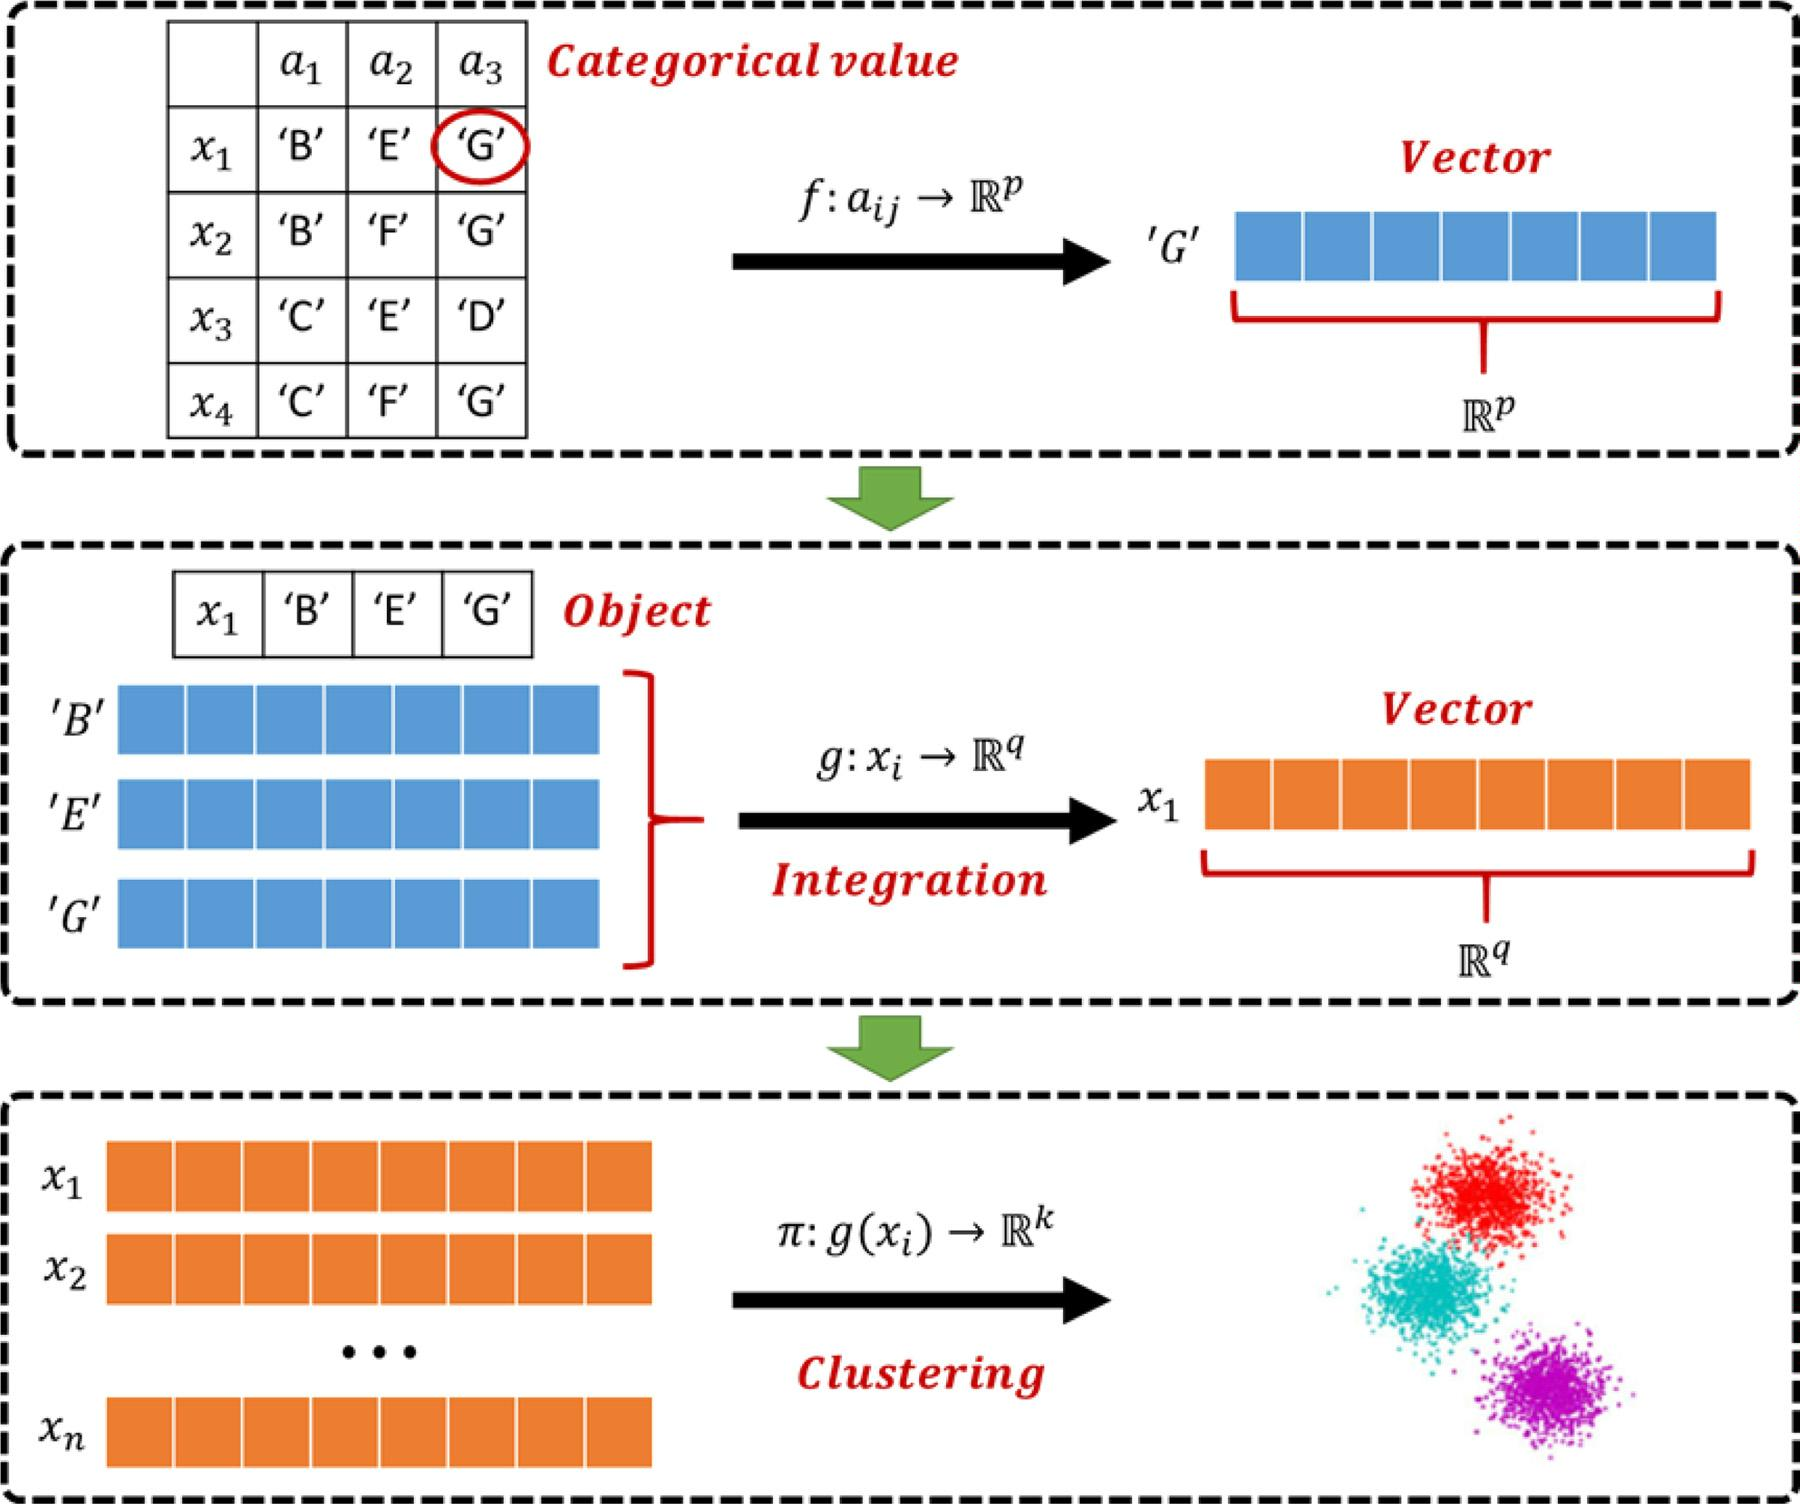
\includegraphics[width=432pt,height=360.96pt]{latexImage_f38a4b042b9f56db589046bde69d2e6e.png}}
\put(238.551,-421.839){\fontsize{6.3761}{1}\usefont{T1}{cmr}{b}{n}\selectfont\color{color_29791}F}
\put(102.624,-512.145){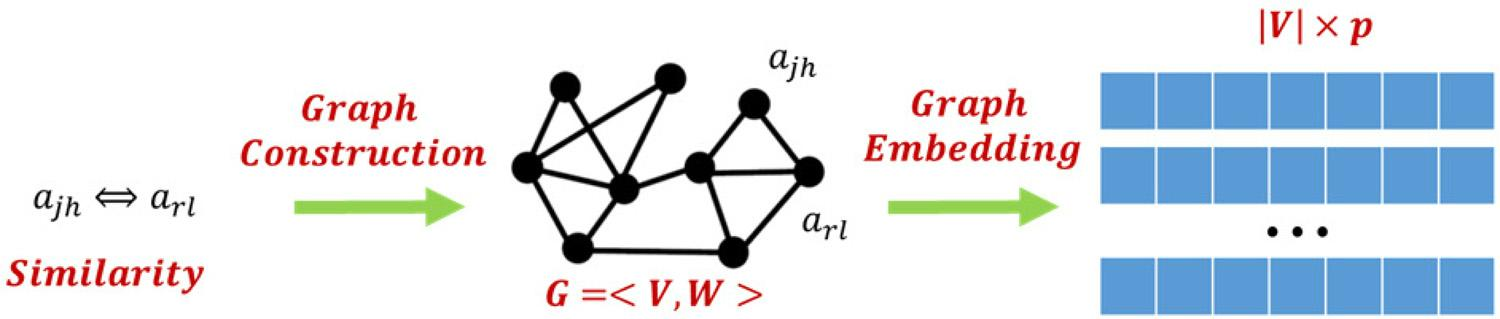
\includegraphics[width=360pt,height=76.55999pt]{latexImage_6f5f022b15224ec0ba4e8514a474eeb6.png}}
\put(218.265,-526.689){\fontsize{6.3761}{1}\usefont{T1}{cmr}{b}{n}\selectfont\color{color_29791}Fig. 2. Representation of categorical value. }
\put(80.169,-553.0139){\fontsize{6.3761}{1}\usefont{T1}{cmr}{b}{n}\selectfont\color{color_29791}Table 2 }
\put(80.169,-561.5821){\fontsize{6.3761}{1}\usefont{T1}{cmr}{m}{n}\selectfont\color{color_29791}Graph embedding methods. }
\put(86.145,-575.703){\fontsize{6.3761}{1}\usefont{T1}{cmr}{m}{n}\selectfont\color{color_29791}Description Equation }
\put(86.19,-589.0949){\fontsize{6.3761}{1}\usefont{T1}{cmr}{m}{n}\selectfont\color{color_29791}NE Z = W }
\put(86.19064,-597.6631){\fontsize{6.3761}{1}\usefont{T1}{cmr}{m}{n}\selectfont\color{color_29791}SE min }
\put(143.637,-598.761){\fontsize{4.4632}{1}\usefont{T1}{cmr}{m}{n}\selectfont\color{color_29791}Z }
\put(147.5699,-597.663){\fontsize{6.3761}{1}\usefont{T1}{cmr}{m}{n}\selectfont\color{color_29791}tr[ Z }
\put(158.991,-595.3499){\fontsize{4.4632}{1}\usefont{T1}{cmr}{m}{n}\selectfont\color{color_29791}T }
\put(162.501,-597.663){\fontsize{7.3325}{1}\usefont{T1}{cmr}{m}{n}\selectfont\color{color_29791}(D −W ) Z] }
\put(86.18945,-606.2312){\fontsize{6.3761}{1}\usefont{T1}{cmr}{m}{n}\selectfont\color{color_29791}NMF min }
\put(143.637,-607.3289){\fontsize{4.4632}{1}\usefont{T1}{cmr}{m}{n}\selectfont\color{color_29791}Z }
\put(147.732,-606.231){\fontsize{7.6513}{1}\usefont{T1}{cmr}{m}{n}\selectfont\color{color_29791}|| W −ZH|| }
\put(179.556,-603.918){\fontsize{4.4632}{1}\usefont{T1}{cmr}{m}{n}\selectfont\color{color_29791}2 }
\put(86.18953,-614.7988){\fontsize{6.3761}{1}\usefont{T1}{cmr}{m}{n}\selectfont\color{color_29791}AE min }
\put(143.637,-616.158){\fontsize{5.3559}{1}\usefont{T1}{cmr}{m}{n}\selectfont\color{color_29791}φ,ψ }
\put(154.284,-614.799){\fontsize{7.6513}{1}\usefont{T1}{cmr}{m}{n}\selectfont\color{color_29791}|| W −ψ(φ(W )) || }
\put(207.168,-612.486){\fontsize{4.4632}{1}\usefont{T1}{cmr}{m}{n}\selectfont\color{color_29791}2 }
\put(22.605,-660.1949){\fontsize{7.9701}{1}\usefont{T1}{cmr}{m}{n}\selectfont\color{color_29791}ber of graph embedding methods have been developed. Some clas- }
\put(22.605,-670.653){\fontsize{7.9701}{1}\usefont{T1}{cmr}{m}{n}\selectfont\color{color_29791}sical methods, such as Non Embedding (NE) where W is directly }
\put(22.605,-681.111){\fontsize{7.9701}{1}\usefont{T1}{cmr}{m}{n}\selectfont\color{color_29791}seen as a feature data, Spectral Embedding (SE) [4] , Nonnegative }
\put(22.605,-691.578){\fontsize{7.9701}{1}\usefont{T1}{cmr}{m}{n}\selectfont\color{color_29791}Matrix Factorization (NMF) [37] , Autoencoder (AE) [38] , are shown }
\put(22.605,-702.036){\fontsize{7.9701}{1}\usefont{T1}{cmr}{m}{n}\selectfont\color{color_29791}in Table 2 . Since the graph embedding operation is implemented }
\put(22.605,-712.494){\fontsize{7.9701}{1}\usefont{T1}{cmr}{m}{n}\selectfont\color{color_29791}on the categorical values and | V | ?n in many data sets, its time }
\put(22.605,-722.961){\fontsize{7.9701}{1}\usefont{T1}{cmr}{m}{n}\selectfont\color{color_29791}complexity should be far less than directly learning the represen- }
\put(22.605,-733.4189){\fontsize{7.9701}{1}\usefont{T1}{cmr}{m}{n}\selectfont\color{color_29791}tation on a data set. }
\put(291.597,-554.634){\fontsize{7.9701}{1}\usefont{T1}{cmr}{m}{n}\selectfont\color{color_29791}2.4. Representation of categorical data }
\put(303.549,-575.5589){\fontsize{7.9701}{1}\usefont{T1}{cmr}{m}{n}\selectfont\color{color_29791}Given f(a }
\put(341.493,-577.5749){\fontsize{5.9776}{1}\usefont{T1}{cmr}{m}{n}\selectfont\color{color_29791}jh }
\put(347.55,-575.5589){\fontsize{9.1656}{1}\usefont{T1}{cmr}{m}{n}\selectfont\color{color_29791}) for each categorical value, in order to get g( x }
\put(526.452,-577.413){\fontsize{5.9776}{1}\usefont{T1}{cmr}{m}{n}\selectfont\color{color_29791}i }
\put(528.972,-575.5589){\fontsize{9.1656}{1}\usefont{T1}{cmr}{m}{n}\selectfont\color{color_29791}) to }
\put(291.597,-586.0169){\fontsize{7.9701}{1}\usefont{T1}{cmr}{m}{n}\selectfont\color{color_29791}represent objects, we need to define the integration operations }
\put(534.048,-580.041){\fontsize{7.9701}{1}\usefont{T1}{cmr}{m}{n}\selectfont\color{color_29791}? }
\put(291.597,-596.4839){\fontsize{7.9701}{1}\usefont{T1}{cmr}{m}{n}\selectfont\color{color_29791}which uses the numerical vectors of categorical values of an object }
\put(291.597,-606.9419){\fontsize{7.9701}{1}\usefont{T1}{cmr}{m}{n}\selectfont\color{color_29791}to represent it. In this paper, we provide two methods which is }
\put(291.597,-617.3999){\fontsize{7.9701}{1}\usefont{T1}{cmr}{m}{n}\selectfont\color{color_29791}shown in Fig. 3 to define }
\put(388.842,-611.424){\fontsize{7.9701}{1}\usefont{T1}{cmr}{m}{n}\selectfont\color{color_29791}? }
\put(400.677,-617.3999){\fontsize{7.9701}{1}\usefont{T1}{cmr}{m}{n}\selectfont\color{color_29791}as follows. }
\put(303.549,-627.8669){\fontsize{7.9701}{1}\usefont{T1}{cmr}{m}{n}\selectfont\color{color_29791}In the first method, }
\put(380.706,-621.8819){\fontsize{7.9701}{1}\usefont{T1}{cmr}{m}{n}\selectfont\color{color_29791}? }
\put(392.712,-627.8669){\fontsize{7.9701}{1}\usefont{T1}{cmr}{m}{n}\selectfont\color{color_29791}is seen as a joint operation and g( x }
\put(527.928,-629.721){\fontsize{5.9776}{1}\usefont{T1}{cmr}{m}{n}\selectfont\color{color_29791}i }
\put(530.457,-627.8669){\fontsize{9.1656}{1}\usefont{T1}{cmr}{m}{n}\selectfont\color{color_29791}) is }
\put(291.597,-638.3249){\fontsize{7.9701}{1}\usefont{T1}{cmr}{m}{n}\selectfont\color{color_29791}defined as }
\put(291.597,-658.071){\fontsize{8.4483}{1}\usefont{T1}{cmr}{m}{n}\selectfont\color{color_29791}g( x }
\put(304.44,-659.709){\fontsize{5.9138}{1}\usefont{T1}{cmr}{m}{n}\selectfont\color{color_29791}i }
\put(306.969,-658.071){\fontsize{9.7156}{1}\usefont{T1}{cmr}{m}{n}\selectfont\color{color_29791}) = [ f (x }
\put(338.172,-659.709){\fontsize{5.9138}{1}\usefont{T1}{cmr}{m}{n}\selectfont\color{color_29791}i 1 }
\put(344.13,-658.071){\fontsize{9.7156}{1}\usefont{T1}{cmr}{m}{n}\selectfont\color{color_29791}) , ···, f (x }
\put(382.083,-659.709){\fontsize{5.9138}{1}\usefont{T1}{cmr}{m}{n}\selectfont\color{color_29791}im }
\put(389.733,-658.071){\fontsize{9.7156}{1}\usefont{T1}{cmr}{m}{n}\selectfont\color{color_29791})] }
\put(291.597,-677.817){\fontsize{7.9701}{1}\usefont{T1}{cmr}{m}{n}\selectfont\color{color_29791}which is a mp-dimensional vector. If f(a }
\put(451.464,-679.8239){\fontsize{5.9776}{1}\usefont{T1}{cmr}{m}{n}\selectfont\color{color_29791}jh }
\put(457.521,-677.817){\fontsize{9.1656}{1}\usefont{T1}{cmr}{m}{n}\selectfont\color{color_29791}) is computed by non }
\put(291.597,-688.2749){\fontsize{7.9701}{1}\usefont{T1}{cmr}{m}{n}\selectfont\color{color_29791}embedding, i.e., Z = W , the squared Euclidean distance between }
\put(291.597,-698.733){\fontsize{7.9701}{1}\usefont{T1}{cmr}{m}{n}\selectfont\color{color_29791}objects is described as }
\put(291.597,-725.571){\fontsize{8.4483}{1}\usefont{T1}{cmr}{m}{n}\selectfont\color{color_29791}d }
\put(296.529,-722.0789){\fontsize{5.9138}{1}\usefont{T1}{cmr}{m}{n}\selectfont\color{color_29791}2 }
\put(300.66,-725.571){\fontsize{9.7156}{1}\usefont{T1}{cmr}{m}{n}\selectfont\color{color_29791}(g( x }
\put(317.211,-727.209){\fontsize{5.9138}{1}\usefont{T1}{cmr}{m}{n}\selectfont\color{color_29791}i }
\put(319.749,-725.571){\fontsize{9.7156}{1}\usefont{T1}{cmr}{m}{n}\selectfont\color{color_29791}) , g( x }
\put(341.358,-727.209){\fontsize{5.9138}{1}\usefont{T1}{cmr}{m}{n}\selectfont\color{color_29791}j }
\put(344.049,-725.571){\fontsize{9.7156}{1}\usefont{T1}{cmr}{m}{n}\selectfont\color{color_29791})) = }
\put(366.396,-714.9149){\fontsize{5.9138}{1}\usefont{T1}{cmr}{m}{n}\selectfont\color{color_29791}m }
\put(362.967,-717.543){\fontsize{8.4483}{1}\usefont{T1}{cmr}{m}{n}\selectfont\color{color_29791}? }
\put(363.264,-736.434){\fontsize{5.9138}{1}\usefont{T1}{cmr}{m}{n}\selectfont\color{color_29791}h =1 }
\put(377.655,-717.543){\fontsize{8.4483}{1}\usefont{T1}{cmr}{m}{n}\selectfont\color{color_29791}? }
\put(376.332,-736.0919){\fontsize{5.9138}{1}\usefont{T1}{cmr}{m}{n}\selectfont\color{color_29791}a }
\put(379.509,-737.4149){\fontsize{4.2242}{1}\usefont{T1}{cmr}{m}{n}\selectfont\color{color_29791}rl }
\put(383.172,-736.0919){\fontsize{5.9138}{1}\usefont{T1}{cmr}{m}{n}\selectfont\color{color_29791}∈ V }
\put(392.343,-717.8399){\fontsize{10.138}{1}\usefont{T1}{cmr}{m}{n}\selectfont\color{color_29791}?}
\put(395.916,-725.571){\fontsize{8.4483}{1}\usefont{T1}{cmr}{m}{n}\selectfont\color{color_29791}W (x }
\put(413.358,-727.371){\fontsize{5.9138}{1}\usefont{T1}{cmr}{m}{n}\selectfont\color{color_29791}ih }
\put(418.884,-725.571){\fontsize{8.4483}{1}\usefont{T1}{cmr}{m}{n}\selectfont\color{color_29791}, a }
\put(427.641,-727.371){\fontsize{5.9138}{1}\usefont{T1}{cmr}{m}{n}\selectfont\color{color_29791}rl }
\put(432.915,-725.571){\fontsize{9.7156}{1}\usefont{T1}{cmr}{m}{n}\selectfont\color{color_29791}) −W (x }
\put(464.811,-727.371){\fontsize{5.9138}{1}\usefont{T1}{cmr}{m}{n}\selectfont\color{color_29791}jh }
\put(470.499,-725.571){\fontsize{8.4483}{1}\usefont{T1}{cmr}{m}{n}\selectfont\color{color_29791}, a }
\put(479.256,-727.371){\fontsize{5.9138}{1}\usefont{T1}{cmr}{m}{n}\selectfont\color{color_29791}rl }
\put(484.53,-725.571){\fontsize{9.7156}{1}\usefont{T1}{cmr}{m}{n}\selectfont\color{color_29791}) }
\put(488.184,-717.8399){\fontsize{10.138}{1}\usefont{T1}{cmr}{m}{n}\selectfont\color{color_29791}?}
\put(491.901,-719.658){\fontsize{5.9138}{1}\usefont{T1}{cmr}{m}{n}\selectfont\color{color_29791}2 }
\put(495.825,-725.571){\fontsize{8.4483}{1}\usefont{T1}{cmr}{m}{n}\selectfont\color{color_29791}. }
\put(280.779,-754.344){\fontsize{6.3761}{1}\usefont{T1}{cmr}{m}{n}\selectfont\color{color_29791}3 }
\end{picture}
\begin{tikzpicture}[overlay]
\path(0pt,0pt);
\draw[color_29791,line width=0.504pt]
(80.169pt, -566.865pt) -- (216.096pt, -566.865pt)
;
\draw[color_29791,line width=0.504pt]
(80.169pt, -580.257pt) -- (216.096pt, -580.257pt)
;
\draw[color_29791,line width=0.504pt]
(80.169pt, -620.109pt) -- (216.096pt, -620.109pt)
;
\end{tikzpicture}
\newpage
\begin{tikzpicture}[overlay]\path(0pt,0pt);\end{tikzpicture}
\begin{picture}(-5,0)(2.5,0)
\put(22.605,-31.13098){\fontsize{6.3761}{1}\usefont{T1}{cmr}{m}{n}\selectfont\color{color_29791}L.}
\put(102.624,-109.296){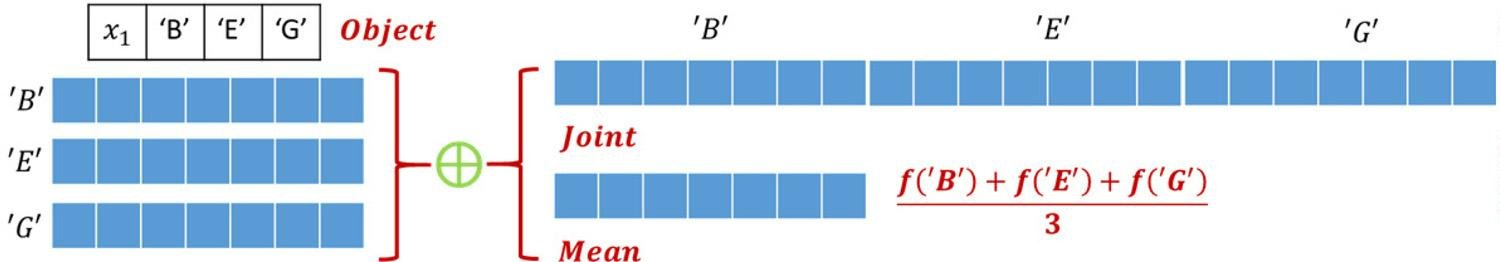
\includegraphics[width=360pt,height=62.88pt]{latexImage_7726cdc940216592535350a761c4dcbe.png}}
\put(219.741,-123.84){\fontsize{6.3761}{1}\usefont{T1}{cmr}{b}{n}\selectfont\color{color_29791}Fig. 3. Representation of categorical data. }
\put(59.145,-150.165){\fontsize{6.3761}{1}\usefont{T1}{cmr}{b}{n}\selectfont\color{color_29791}Table 3 }
\put(59.145,-158.7332){\fontsize{6.3761}{1}\usefont{T1}{cmr}{m}{n}\selectfont\color{color_29791}Description of data sets. }
\put(65.121,-172.8539){\fontsize{6.3761}{1}\usefont{T1}{cmr}{m}{n}\selectfont\color{color_29791}Data set n m k Type }
\put(65.166,-186.246){\fontsize{6.3761}{1}\usefont{T1}{cmr}{m}{n}\selectfont\color{color_29791}Soybean 47 21 4 Categorical }
\put(65.166,-194.8142){\fontsize{6.3761}{1}\usefont{T1}{cmr}{m}{n}\selectfont\color{color_29791}Zoo 101 16 7 Categorical }
\put(65.16728,-203.3824){\fontsize{6.3761}{1}\usefont{T1}{cmr}{m}{n}\selectfont\color{color_29791}Heart disease 303 8 2 Categorical }
\put(65.16855,-211.9506){\fontsize{6.3761}{1}\usefont{T1}{cmr}{m}{n}\selectfont\color{color_29791}Breast cancer 699 9 2 Categorical }
\put(65.17046,-220.5188){\fontsize{6.3761}{1}\usefont{T1}{cmr}{m}{n}\selectfont\color{color_29791}Dermatology 366 33 6 Categorical }
\put(65.1711,-229.087){\fontsize{6.3761}{1}\usefont{T1}{cmr}{m}{n}\selectfont\color{color_29791}Letters(E,F) 1543 16 2 Categorical }
\put(65.1711,-237.6552){\fontsize{6.3761}{1}\usefont{T1}{cmr}{m}{n}\selectfont\color{color_29791}DNA 3,190 60 3 Categorical }
\put(65.17046,-246.2234){\fontsize{6.3761}{1}\usefont{T1}{cmr}{m}{n}\selectfont\color{color_29791}Mushroom 8,124 22 2 Categorical }
\put(65.1711,-254.7916){\fontsize{6.3761}{1}\usefont{T1}{cmr}{m}{n}\selectfont\color{color_29791}Iris 150 4 3 Numerical }
\put(65.1711,-263.3598){\fontsize{6.3761}{1}\usefont{T1}{cmr}{m}{n}\selectfont\color{color_29791}Isolet 1,560 617 26}
\put(185.5557,-263.358){\fontsize{6.3761}{1}\usefont{T1}{cmr}{m}{n}\selectfont\color{color_29791} Numerical }
\put(65.16601,-271.9262){\fontsize{6.3761}{1}\usefont{T1}{cmr}{m}{n}\selectfont\color{color_29791}COIL20 1,140 1024 20 Numerical }
\put(65.16664,-280.4944){\fontsize{6.3761}{1}\usefont{T1}{cmr}{m}{n}\selectfont\color{color_29791}OpticalDigits 5,620 64 10 Numerical }
\put(65.16664,-289.0626){\fontsize{6.3761}{1}\usefont{T1}{cmr}{m}{n}\selectfont\color{color_29791}PenDigits 10,992 36 10 Numerical }
\put(22.605,-322.461){\fontsize{7.9701}{1}\usefont{T1}{cmr}{m}{n}\selectfont\color{color_29791}The distance does not directly measure the dissimilarity of be- }
\put(22.605,-332.928){\fontsize{7.9701}{1}\usefont{T1}{cmr}{m}{n}\selectfont\color{color_29791}tween corresponding categorical values of two objects but evaluate }
\put(22.605,-343.386){\fontsize{7.9701}{1}\usefont{T1}{cmr}{m}{n}\selectfont\color{color_29791}the difference between the similarity of them with all the categor- }
\put(22.605,-353.844){\fontsize{7.9701}{1}\usefont{T1}{cmr}{m}{n}\selectfont\color{color_29791}ical values. This indicates that the inherent similarity between cat- }
\put(22.605,-364.3109){\fontsize{7.9701}{1}\usefont{T1}{cmr}{m}{n}\selectfont\color{color_29791}egorical values is sufiiciently considered in the data representation. }
\put(34.557,-374.769){\fontsize{7.9701}{1}\usefont{T1}{cmr}{m}{n}\selectfont\color{color_29791}In the second method, }
\put(124.476,-368.793){\fontsize{7.9701}{1}\usefont{T1}{cmr}{m}{n}\selectfont\color{color_29791}? }
\put(136.923,-374.769){\fontsize{7.9701}{1}\usefont{T1}{cmr}{m}{n}\selectfont\color{color_29791}is defined as a mean operation and }
\put(22.605,-385.227){\fontsize{7.9701}{1}\usefont{T1}{cmr}{m}{n}\selectfont\color{color_29791}then g( x }
\put(54.564,-387.081){\fontsize{5.9776}{1}\usefont{T1}{cmr}{m}{n}\selectfont\color{color_29791}i }
\put(57.084,-385.227){\fontsize{9.1656}{1}\usefont{T1}{cmr}{m}{n}\selectfont\color{color_29791}) becomes }
\put(22.605,-408.483){\fontsize{8.4483}{1}\usefont{T1}{cmr}{m}{n}\selectfont\color{color_29791}g( x }
\put(35.448,-410.121){\fontsize{5.9138}{1}\usefont{T1}{cmr}{m}{n}\selectfont\color{color_29791}i }
\put(37.977,-408.483){\fontsize{9.7156}{1}\usefont{T1}{cmr}{m}{n}\selectfont\color{color_29791}) = }
\put(55.338,-402.5609){\fontsize{8.4483}{1}\usefont{T1}{cmr}{m}{n}\selectfont\color{color_29791}1 }
\end{picture}
\begin{tikzpicture}[overlay]
\path(0pt,0pt);
\draw[color_29791,line width=0.396pt]
(54.132pt, -406.368pt) -- (61.44pt, -406.368pt)
;
\end{tikzpicture}
\begin{picture}(-5,0)(2.5,0)
\put(54.132,-414.486){\fontsize{8.4483}{1}\usefont{T1}{cmr}{m}{n}\selectfont\color{color_29791}m }
\put(67.452,-397.827){\fontsize{5.9138}{1}\usefont{T1}{cmr}{m}{n}\selectfont\color{color_29791}m }
\put(64.032,-400.455){\fontsize{8.4483}{1}\usefont{T1}{cmr}{m}{n}\selectfont\color{color_29791}? }
\put(65.508,-419.184){\fontsize{5.9138}{1}\usefont{T1}{cmr}{m}{n}\selectfont\color{color_29791}j=1 }
\put(78.729,-408.483){\fontsize{8.4483}{1}\usefont{T1}{cmr}{m}{n}\selectfont\color{color_29791}f(x }
\put(90.537,-410.121){\fontsize{5.9138}{1}\usefont{T1}{cmr}{m}{n}\selectfont\color{color_29791}ij }
\put(95.766,-408.483){\fontsize{9.7156}{1}\usefont{T1}{cmr}{m}{n}\selectfont\color{color_29791}) }
\put(22.605,-434.133){\fontsize{7.9701}{1}\usefont{T1}{cmr}{m}{n}\selectfont\color{color_29791}which is a p-dimensional vector. Compared to the joint operation, }
\put(22.605,-444.5909){\fontsize{7.9701}{1}\usefont{T1}{cmr}{m}{n}\selectfont\color{color_29791}this representation has low dimensions and smooth feature values. }
\put(22.605,-466.2539){\fontsize{7.9701}{1}\usefont{T1}{cmr}{m}{n}\selectfont\color{color_29791}2.5. Clustering categorical data }
\put(34.557,-487.17){\fontsize{7.9701}{1}\usefont{T1}{cmr}{m}{n}\selectfont\color{color_29791}Given g( x }
\put(71.331,-489.024){\fontsize{5.9776}{1}\usefont{T1}{cmr}{m}{n}\selectfont\color{color_29791}i }
\put(73.851,-487.17){\fontsize{9.1656}{1}\usefont{T1}{cmr}{m}{n}\selectfont\color{color_29791}) for 1 ≤i ≤n , we can employ one of classical clus- }
\put(22.605,-497.637){\fontsize{7.9701}{1}\usefont{T1}{cmr}{m}{n}\selectfont\color{color_29791}tering algorithms for numerical data to define the clustering func- }
\put(22.605,-508.095){\fontsize{7.9701}{1}\usefont{T1}{cmr}{m}{n}\selectfont\color{color_29791}tion π(. ) . The clustering algorithm includes k -means, linkage, spec- }
\put(291.597,-151.785){\fontsize{7.9701}{1}\usefont{T1}{cmr}{m}{n}\selectfont\color{color_29791}tral clustering and so on. Therefore, the overall clustering process }
\put(291.597,-162.252){\fontsize{7.9701}{1}\usefont{T1}{cmr}{m}{n}\selectfont\color{color_29791}in the proposed framework is described in Algorithm 1 , which is }
\end{picture}
\begin{tikzpicture}[overlay]
\path(0pt,0pt);
\draw[color_29791,line width=0.801pt]
(291.597pt, -174.433pt) -- (542.661pt, -174.433pt)
;
\end{tikzpicture}
\begin{picture}(-5,0)(2.5,0)
\put(291.597,-183.141){\fontsize{7.9701}{1}\usefont{T1}{cmr}{b}{n}\selectfont\color{color_29791}Algorithm 1 CDC\_DR. }
\end{picture}
\begin{tikzpicture}[overlay]
\path(0pt,0pt);
\draw[color_29791,line width=0.405pt]
(291.597pt, -186.934pt) -- (542.661pt, -186.934pt)
;
\end{tikzpicture}
\begin{picture}(-5,0)(2.5,0)
\put(291.597,-195.48){\fontsize{7.9701}{1}\usefont{T1}{cmr}{b}{n}\selectfont\color{color_29791}Input : X, k }
\put(291.597,-205.938){\fontsize{7.9701}{1}\usefont{T1}{cmr}{b}{n}\selectfont\color{color_29791}Parameter : ‘Set-Similarity Measure’, ‘Graph Embedding Method’, }
\put(291.597,-216.405){\fontsize{7.9701}{1}\usefont{T1}{cmr}{m}{n}\selectfont\color{color_29791}‘Integration Operation’, ‘Clustering Algorithm’ }
\put(291.597,-226.863){\fontsize{7.9701}{1}\usefont{T1}{cmr}{b}{n}\selectfont\color{color_29791}Output : UBuild a graph G = < V, W > of categorical values by the }
\put(291.597,-237.321){\fontsize{7.9701}{1}\usefont{T1}{cmr}{m}{n}\selectfont\color{color_29791}selected similarity measure;Get a representation matrix of categor- }
\put(291.597,-247.788){\fontsize{7.9701}{1}\usefont{T1}{cmr}{m}{n}\selectfont\color{color_29791}ical values f(V ) by the selected graph embedding method;Get a }
\put(291.597,-258.246){\fontsize{7.9701}{1}\usefont{T1}{cmr}{m}{n}\selectfont\color{color_29791}representation matrix of objects g(X) by the selected integration }
\put(291.597,-268.704){\fontsize{7.9701}{1}\usefont{T1}{cmr}{m}{n}\selectfont\color{color_29791}operation;Compute U = π(g(X)) by the selected clustering algo- }
\put(291.597,-279.171){\fontsize{7.9701}{1}\usefont{T1}{cmr}{m}{n}\selectfont\color{color_29791}rithm; return U }
\end{picture}
\begin{tikzpicture}[overlay]
\path(0pt,0pt);
\draw[color_29791,line width=0.405pt]
(291.597pt, -282.586pt) -- (542.661pt, -282.586pt)
;
\end{tikzpicture}
\begin{picture}(-5,0)(2.5,0)
\put(291.597,-301.662){\fontsize{7.9701}{1}\usefont{T1}{cmr}{m}{n}\selectfont\color{color_29791}called “CDC\_DR”. According to the description of the algorithm, }
\put(291.597,-312.129){\fontsize{7.9701}{1}\usefont{T1}{cmr}{m}{n}\selectfont\color{color_29791}the computation cost of the proposed framework is made up of }
\put(291.597,-322.587){\fontsize{7.9701}{1}\usefont{T1}{cmr}{m}{n}\selectfont\color{color_29791}constructing graph ( O (| V | }
\put(388.338,-319.698){\fontsize{5.9776}{1}\usefont{T1}{cmr}{m}{n}\selectfont\color{color_29791}2 }
\put(392.298,-322.587){\fontsize{7.9701}{1}\usefont{T1}{cmr}{m}{n}\selectfont\color{color_29791}n ) ), graph embedding, integration oper- }
\put(291.597,-333.045){\fontsize{7.9701}{1}\usefont{T1}{cmr}{m}{n}\selectfont\color{color_29791}ation ( O (nmp) ) and numerical data clustering ( O (nqk ) if k -means }
\put(291.597,-343.512){\fontsize{7.9701}{1}\usefont{T1}{cmr}{m}{n}\selectfont\color{color_29791}is selected). For the graph embedding, different methods need dif- }
\put(291.597,-353.9699){\fontsize{7.9701}{1}\usefont{T1}{cmr}{m}{n}\selectfont\color{color_29791}ferent computational costs. The time complexities of NE, SE, NMF }
\put(291.597,-364.428){\fontsize{7.9701}{1}\usefont{T1}{cmr}{m}{n}\selectfont\color{color_29791}and AE (is set as the three-level network) are O (1) , O (| V | }
\put(528.693,-361.539){\fontsize{5.9776}{1}\usefont{T1}{cmr}{m}{n}\selectfont\color{color_29791}2 }
\put(533.247,-364.428){\fontsize{7.9701}{1}\usefont{T1}{cmr}{m}{n}\selectfont\color{color_29791}p) , }
\put(291.597,-374.895){\fontsize{7.9701}{1}\usefont{T1}{cmr}{m}{n}\selectfont\color{color_29791}O (| V | }
\put(311.793,-371.9969){\fontsize{5.9776}{1}\usefont{T1}{cmr}{m}{n}\selectfont\color{color_29791}2 }
\put(316.338,-374.895){\fontsize{7.9701}{1}\usefont{T1}{cmr}{m}{n}\selectfont\color{color_29791}p + | V | p }
\put(346.272,-371.9969){\fontsize{5.9776}{1}\usefont{T1}{cmr}{m}{n}\selectfont\color{color_29791}2 }
\put(350.547,-374.895){\fontsize{9.1656}{1}\usefont{T1}{cmr}{m}{n}\selectfont\color{color_29791}) and O (| V | }
\put(395.826,-371.9969){\fontsize{5.9776}{1}\usefont{T1}{cmr}{m}{n}\selectfont\color{color_29791}3 }
\put(400.38,-374.895){\fontsize{7.9701}{1}\usefont{T1}{cmr}{m}{n}\selectfont\color{color_29791}p) , respectively. We can see that the }
\put(291.597,-385.353){\fontsize{7.9701}{1}\usefont{T1}{cmr}{m}{n}\selectfont\color{color_29791}computational cost of NE is the lowest, since it does not represent }
\put(291.597,-395.8109){\fontsize{7.9701}{1}\usefont{T1}{cmr}{m}{n}\selectfont\color{color_29791}graph. The time complexity of NMF is squared with | V | and p. AE }
\put(291.597,-406.269){\fontsize{7.9701}{1}\usefont{T1}{cmr}{m}{n}\selectfont\color{color_29791}needs high training costs, compared to other methods. For spec- }
\put(291.597,-416.736){\fontsize{7.9701}{1}\usefont{T1}{cmr}{m}{n}\selectfont\color{color_29791}tral embedding (SE), its cost is mainly from eigen decomposition. }
\put(291.597,-427.1939){\fontsize{7.9701}{1}\usefont{T1}{cmr}{m}{n}\selectfont\color{color_29791}If the number of nodes in a graph is not large, the computational }
\put(291.597,-437.652){\fontsize{7.9701}{1}\usefont{T1}{cmr}{m}{n}\selectfont\color{color_29791}cost can be acceptable. }
\put(291.597,-455.787){\fontsize{7.9701}{1}\usefont{T1}{cmr}{b}{n}\selectfont\color{color_29791}3. Experiment analysis }
\put(291.597,-476.712){\fontsize{7.9701}{1}\usefont{T1}{cmr}{m}{n}\selectfont\color{color_29791}3.1. Experiment environment }
\put(303.549,-497.637){\fontsize{7.9701}{1}\usefont{T1}{cmr}{m}{n}\selectfont\color{color_29791}In order to examine the performance of the proposed frame- }
\put(291.597,-508.095){\fontsize{7.9701}{1}\usefont{T1}{cmr}{m}{n}\selectfont\color{color_29791}work, we select Ochiai coefiicient as set-similarity measure and k - }
\put(25.593,-533.07){\fontsize{6.3761}{1}\usefont{T1}{cmr}{b}{n}\selectfont\color{color_29791}Table 4 }
\put(25.593,-541.6382){\fontsize{6.3761}{1}\usefont{T1}{cmr}{m}{n}\selectfont\color{color_29791}The proposed framework for clustering categorical data. }
\put(31.569,-555.759){\fontsize{6.3761}{1}\usefont{T1}{cmr}{m}{n}\selectfont\color{color_29791}Dataset Index NE SE NMF AE Average Max }
\put(95.694,-569.016){\fontsize{6.3761}{1}\usefont{T1}{cmr}{m}{n}\selectfont\color{color_29791}Joint Mean Joint Mean Joint Mean Joint Mean }
\put(31.614,-582.408){\fontsize{6.3761}{1}\usefont{T1}{cmr}{m}{n}\selectfont\color{color_29791}Soybean ARI 0.7784 ±0.21 0.8312 ±0.21 0.7498 ±0.2 0.8572 ±0.19 0.813 ±0.21 0.8381 ±0.19 0.7774 ±0.2 0.8159 ±0.21 0.8076 ±0.2 0.8572 ±0.21 }
\put(69.66083,-590.9762){\fontsize{6.3761}{1}\usefont{T1}{cmr}{m}{n}\selectfont\color{color_29791}NMI 0.8787 ±0.12 0.9058 ±0.12 0.8627 ±0.11 0.9254 ±0.1 0.8974 ±0.12 0.9116 ±0.1 0.879 ±0.11 0.8996 ±0.12 0.895 ±0.11 }
\put(491.8699,-590.976){\fontsize{6.3761}{1}\usefont{T1}{cmr}{m}{n}\selectfont\color{color_29791}0.9254 ±0.12 }
\put(31.61303,-599.5442){\fontsize{6.3761}{1}\usefont{T1}{cmr}{m}{n}\selectfont\color{color_29791}Zoo ARI 0.6867 ±0.17 0.6765 ±0.15 0.6414 ±0.14 0.6623 ±0.14 0.666 ±0.16 0.6584 ±0.14 0.7069 ±0.14 0.653 ±0.14 0.6689 ±0.15 0.7069 ±0.17 }
\put(69.65859,-608.1124){\fontsize{6.3761}{1}\usefont{T1}{cmr}{m}{n}\selectfont\color{color_29791}NMI 0.7949 ±0.08 0.8026 ±0.07 0.7777 ±0.07 0.7823 ±0.06 0.7859 ±0.07 0.7925 ±0.07 0.7999 ±0.06 0.7684 ±0.06 }
\put(447.8525,-608.1119){\fontsize{6.3761}{1}\usefont{T1}{cmr}{m}{n}\selectfont\color{color_29791}0.788 ±0.07 0.8026 ±0.08 }
\put(31.61432,-616.6801){\fontsize{6.3761}{1}\usefont{T1}{cmr}{m}{n}\selectfont\color{color_29791}Heart ARI 0.4024 ±0.06 0.4424 ±0.00 0.4232 ±0.06 0.4208 ±0.00 0.4187 ±0.01 0.4384 ±0.01 0.3892 ±0.09 0.3169 ±0.06 0.4065 ±0.04 0.4424 ±0.09 }
\put(31.61623,-625.2483){\fontsize{6.3761}{1}\usefont{T1}{cmr}{m}{n}\selectfont\color{color_29791}disease NMI 0.3144 ±0.05 0.3491 ±0.00 0.3342 ±0.05 0.3297 ±0.00 0.3278 ±0.01 0.3454 ±0.01 0.3086 ±}
\put(385.2864,-625.248){\fontsize{6.3761}{1}\usefont{T1}{cmr}{m}{n}\selectfont\color{color_29791}0.07 0.2646 ±0.03 0.3217 ±0.03 0.3491 ±0.07 }
\put(31.61433,-633.8162){\fontsize{6.3761}{1}\usefont{T1}{cmr}{m}{n}\selectfont\color{color_29791}Derm- ARI 0.6273 ±0.16 0.589 ±0.12 0.6887 ±0.16 0.5449 ±0.09 0.6297 ±0.16 0.5742 ±0.11 0.6941 ±0.14 0.5347 ±0.06 0.6103 ±0.12 0.6941 ±0.16 }
\put(31.61625,-642.3755){\fontsize{6.3761}{1}\usefont{T1}{cmr}{m}{n}\selectfont\color{color_29791}atology NMI 0.7931 ±0.09 0.7586 ±0.07 0.8183 ±0.08 0.7279 ±0.03 0.7925 ±0.09 0.7434}
\put(336.2394,-642.3749){\fontsize{6.3761}{1}\usefont{T1}{cmr}{m}{n}\selectfont\color{color_29791} ±0.06 0.8247 ±0.07 0.6558 ±0.01 0.7643 ±0.06 0.8247 ±0.09 }
\put(31.61421,-650.9431){\fontsize{6.3761}{1}\usefont{T1}{cmr}{m}{n}\selectfont\color{color_29791}Breast ARI 0.8988 ±0.00 0.8988 ±0.00 0.8988 ±0.00 0.9043 ±0.00 0.8988 ±0.00 0.8988 ±0.00 0.8026 ±0.19 0.8727 ±0.03 0.8842 ±0.03 0.9043 ±0.19 }
\put(31.61421,-659.5113){\fontsize{6.3761}{1}\usefont{T1}{cmr}{m}{n}\selectfont\color{color_29791}cancer NMI 0.8269 ±0.00 0.8311 ±0.00 0.8269 ±0.00 0.8377 ±0.00}
\put(266.1062,-659.511){\fontsize{6.3761}{1}\usefont{T1}{cmr}{m}{n}\selectfont\color{color_29791} 0.8269 ±0.00 0.8311 ±0.00 0.7252 ±0.18 0.7951 ±0.03 0.8126 ±0.03 0.8377 ±0.18 }
\put(31.61428,-668.0792){\fontsize{6.3761}{1}\usefont{T1}{cmr}{m}{n}\selectfont\color{color_29791}DNA ARI 0.68 ±0.09 0.2442 ±0.03 0.5077 ±0.12 0.6799 ±0.13 0.1605 ±0.05 0.0618 ±0.00 0.5085 ±0.15 0.3542 ±0.12 0.3996 ±0.09 0.6800 ±0.15 }
\put(69.66047,-676.6474){\fontsize{6.3761}{1}\usefont{T1}{cmr}{m}{n}\selectfont\color{color_29791}NMI 0.6425 ±0.07 0.2644 ±0.03 0.4739 ±0.09}
\put(222.0999,-676.6469){\fontsize{6.3761}{1}\usefont{T1}{cmr}{m}{n}\selectfont\color{color_29791} 0.6344 ±0.11 0.1731 ±0.04 0.0665 ±0.01 0.5225 ±0.11 0.3699 ±0.09 0.3934 ±0.07 0.6425 ±0.11 }
\put(31.61455,-685.2151){\fontsize{6.3761}{1}\usefont{T1}{cmr}{m}{n}\selectfont\color{color_29791}Letters ARI 0.3741 ±0.26 0.4007 ±0.2 0.4862 ±0.23 0.4404 ±0.19 0.5247 ±0.00 0.3668 ±0.00 0.2902 ±0.21 0.3902 ±0.19 0.4092 ±0.16 0.5247 ±0.26 }
\put(69.65946,-693.7833){\fontsize{6.3761}{1}\usefont{T1}{cmr}{m}{n}\selectfont\color{color_29791}NMI 0.3598 ±0.25 0.3778 ±0.19}
\put(178.1014,-693.783){\fontsize{6.3761}{1}\usefont{T1}{cmr}{m}{n}\selectfont\color{color_29791} 0.4641 ±0.21 0.4275 ±0.15 0.5124 ±0.00 0.3084 ±0.00 0.2665 ±0.19 0.3469 ±0.16 0.3829 ±0.14 0.5124 ±0.25 }
\put(31.61497,-702.3512){\fontsize{6.3761}{1}\usefont{T1}{cmr}{m}{n}\selectfont\color{color_29791}Mush- ARI 0.3176 ±0.23 0.3909 ±0.23 0.6165 ±0.09 0.607 ±0.09 0.6174 ±0.02 0.609 ±0.02 0.383 ±0.25 0.3213 ±0.21 0.4828 ±0.14 0.6174 ±0.25 }
\put(31.61752,-710.9194){\fontsize{6.3761}{1}\usefont{T1}{cmr}{m}{n}\selectfont\color{color_29791}room NMI 0.3599 }
\put(116.1927,-710.9189){\fontsize{6.3761}{1}\usefont{T1}{cmr}{m}{n}\selectfont\color{color_29791}±0.17 0.4010 ±0.18 0.5845 ±0.08 0.5734 ±0.08 0.5883 ±0.04 0.5658 ±0.04 0.3858 ±0.21 0.3605 ±0.14 0.4774 ±0.12 0.5883 ±0.21 }
\put(280.779,-754.344){\fontsize{6.3761}{1}\usefont{T1}{cmr}{m}{n}\selectfont\color{color_29791}4 }
\end{picture}
\begin{tikzpicture}[overlay]
\path(0pt,0pt);
\draw[color_29791,line width=0.504pt]
(59.145pt, -164.016pt) -- (237.129pt, -164.016pt)
;
\draw[color_29791,line width=0.504pt]
(59.145pt, -177.408pt) -- (237.129pt, -177.408pt)
;
\draw[color_29791,line width=0.504pt]
(59.145pt, -294.372pt) -- (237.129pt, -294.372pt)
;
\draw[color_29791,line width=0.504pt]
(25.593pt, -546.921pt) -- (539.673pt, -546.921pt)
;
\draw[color_29791,line width=0.504pt]
(95.694pt, -560.673pt) -- (181.554pt, -560.673pt)
;
\draw[color_29791,line width=0.504pt]
(183.723pt, -560.673pt) -- (269.583pt, -560.673pt)
;
\draw[color_29791,line width=0.504pt]
(271.761pt, -560.673pt) -- (357.621pt, -560.673pt)
;
\draw[color_29791,line width=0.504pt]
(359.79pt, -560.673pt) -- (445.65pt, -560.673pt)
;
\draw[color_29791,line width=0.504pt]
(447.828pt, -560.673pt) -- (489.678pt, -560.673pt)
;
\draw[color_29791,line width=0.504pt]
(491.847pt, -560.673pt) -- (533.697pt, -560.673pt)
;
\draw[color_29791,line width=0.504pt]
(25.59299pt, -573.561pt) -- (539.673pt, -573.561pt)
;
\draw[color_29791,line width=0.504pt]
(25.59299pt, -716.229pt) -- (539.673pt, -716.229pt)
;
\end{tikzpicture}
\newpage
\begin{tikzpicture}[overlay]\path(0pt,0pt);\end{tikzpicture}
\begin{picture}(-5,0)(2.5,0)
\put(22.605,-31.13098){\fontsize{6.3761}{1}\usefont{T1}{cmr}{m}{n}\selectfont\color{color_29791}L.}
\put(102.624,-271.296){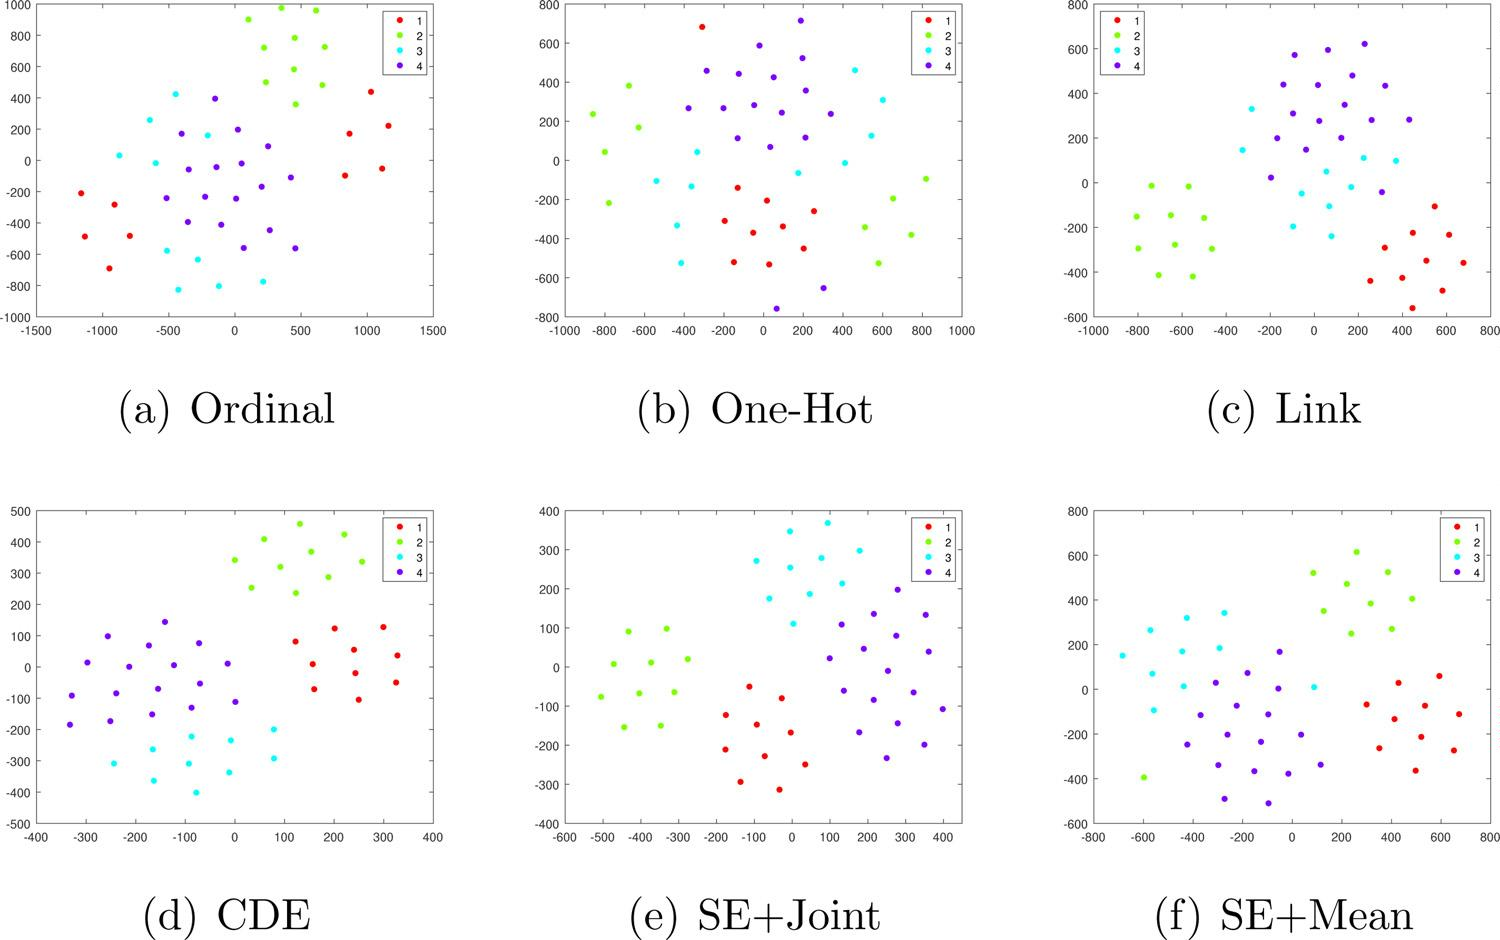
\includegraphics[width=360pt,height=225.48pt]{latexImage_e3354728c6dcaeff863b98f64a3efb87.png}}
\put(201.552,-285.84){\fontsize{6.3761}{1}\usefont{T1}{cmr}{b}{n}\selectfont\color{color_29791}F}
\put(102.624,-543.087){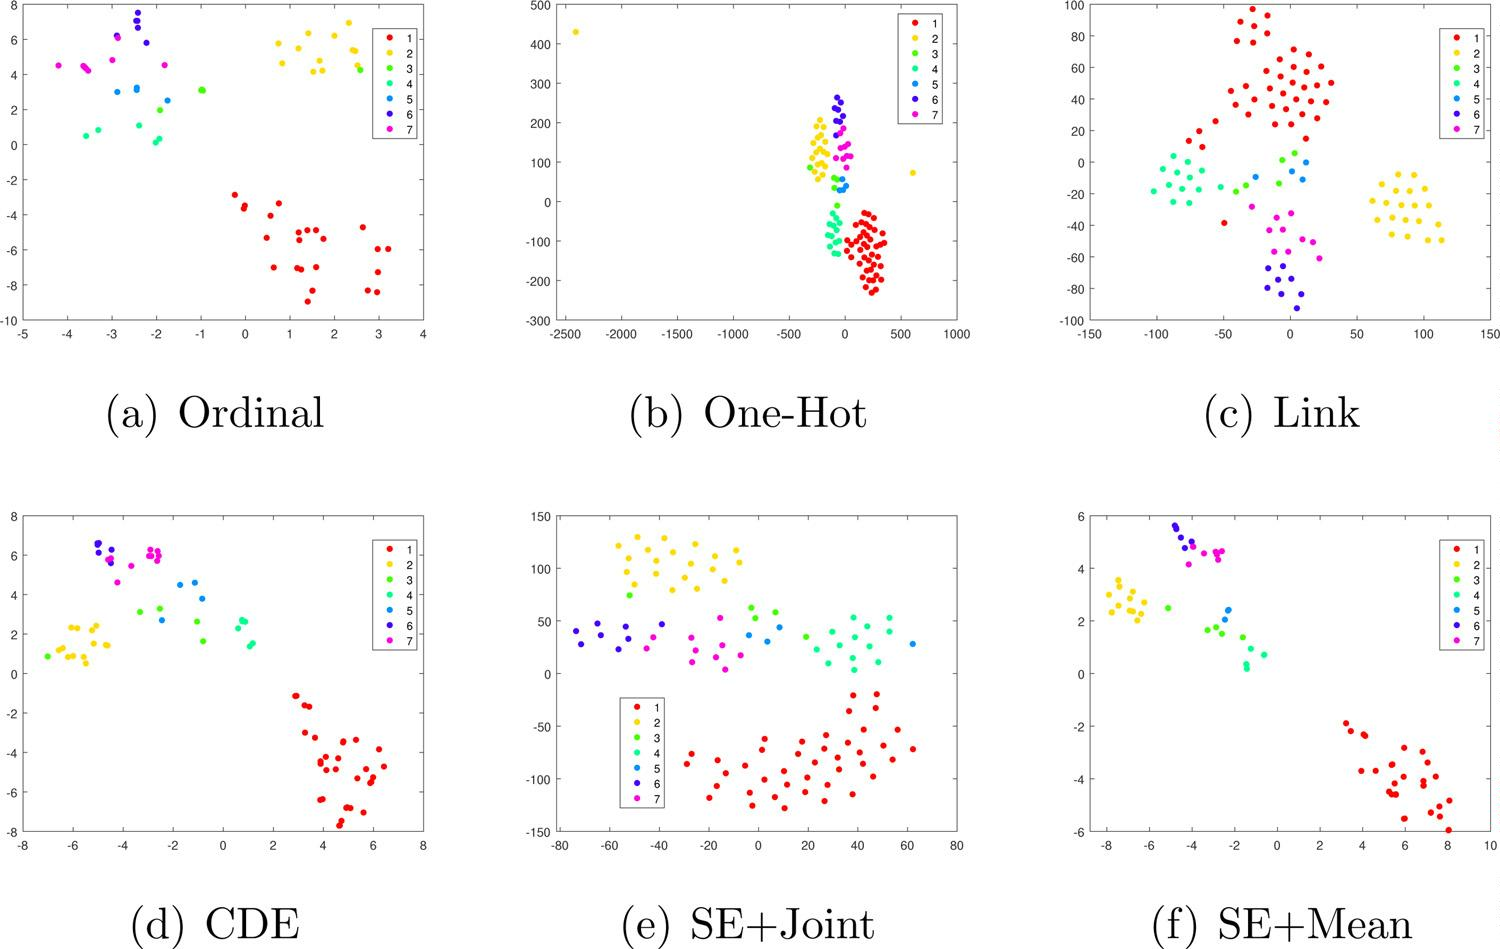
\includegraphics[width=360pt,height=227.64pt]{latexImage_9977e254815f0a8d33f32d2efeba2980.png}}
\put(208.455,-557.631){\fontsize{6.3761}{1}\usefont{T1}{cmr}{b}{n}\selectfont\color{color_29791}Fig. 5. Scatter plots of different methods on Zoo. }
\put(22.605,-601.515){\fontsize{7.9701}{1}\usefont{T1}{cmr}{m}{n}\selectfont\color{color_29791}means as clustering algorithm. Furthermore, we test four graph- }
\put(22.605,-611.9819){\fontsize{7.9701}{1}\usefont{T1}{cmr}{m}{n}\selectfont\color{color_29791}embedding methods including NE, SE, NMF and AE, and two in- }
\put(22.605,-622.4399){\fontsize{7.9701}{1}\usefont{T1}{cmr}{m}{n}\selectfont\color{color_29791}tegration operations including Joint and Mean in this framework. }
\put(22.605,-632.898){\fontsize{7.9701}{1}\usefont{T1}{cmr}{m}{n}\selectfont\color{color_29791}While using NE, we know pequal to the sum of the numbers of }
\put(22.605,-643.3649){\fontsize{7.9701}{1}\usefont{T1}{cmr}{m}{n}\selectfont\color{color_29791}categorical values of all the features. For SE, NMF and AE, we set }
\put(23.199,-653.823){\fontsize{7.9701}{1}\usefont{T1}{cmr}{m}{n}\selectfont\color{color_29791}pto their average number. We compare the proposed framework }
\put(22.605,-664.281){\fontsize{7.9701}{1}\usefont{T1}{cmr}{m}{n}\selectfont\color{color_29791}with categorical data clustering methods based on five different }
\put(22.605,-674.748){\fontsize{7.9701}{1}\usefont{T1}{cmr}{m}{n}\selectfont\color{color_29791}categorical data encodings: k -modes [13] , k -means with ordinal en- }
\put(22.605,-685.206){\fontsize{7.9701}{1}\usefont{T1}{cmr}{m}{n}\selectfont\color{color_29791}coding, one-hot encoding [26] , link-graph encoding [28] , and cou- }
\put(22.605,-695.664){\fontsize{7.9701}{1}\usefont{T1}{cmr}{m}{n}\selectfont\color{color_29791}pled data embedding [29] . Besides, we set the number of clusters }
\put(22.605,-706.1219){\fontsize{7.9701}{1}\usefont{T1}{cmr}{m}{n}\selectfont\color{color_29791}on each tested data set to its “true”number of classes. The ex- }
\put(22.605,-716.589){\fontsize{7.9701}{1}\usefont{T1}{cmr}{m}{n}\selectfont\color{color_29791}periments are conducted on an Intel i9-7940X@3.10GHz personal }
\put(22.605,-727.0469){\fontsize{7.9701}{1}\usefont{T1}{cmr}{m}{n}\selectfont\color{color_29791}computer with 128G RAM and Matlab 2016b. }
\put(303.549,-601.5149){\fontsize{7.9701}{1}\usefont{T1}{cmr}{m}{n}\selectfont\color{color_29791}In the experiments, we consider two scenarios of comparisons. }
\put(291.597,-611.9819){\fontsize{7.9701}{1}\usefont{T1}{cmr}{m}{n}\selectfont\color{color_29791}The one is clustering categorical data sets. The second is clustering }
\put(291.597,-622.4399){\fontsize{7.9701}{1}\usefont{T1}{cmr}{m}{n}\selectfont\color{color_29791}ensemble, where multiple clustering results of a data set are seen }
\put(291.597,-632.898){\fontsize{7.9701}{1}\usefont{T1}{cmr}{m}{n}\selectfont\color{color_29791}as its categorical features. A clustering ensemble problem can be }
\put(291.597,-643.3649){\fontsize{7.9701}{1}\usefont{T1}{cmr}{m}{n}\selectfont\color{color_29791}seen as a categorical data clustering problem [39,40] . Therefore, in }
\put(291.597,-653.823){\fontsize{7.9701}{1}\usefont{T1}{cmr}{m}{n}\selectfont\color{color_29791}this paper, we also show the performance of the proposed frame- }
\put(291.597,-664.281){\fontsize{7.9701}{1}\usefont{T1}{cmr}{m}{n}\selectfont\color{color_29791}work on clustering ensemble. The comparisons are carried out on }
\put(291.597,-674.748){\fontsize{7.9701}{1}\usefont{T1}{cmr}{m}{n}\selectfont\color{color_29791}13 benchmark data sets including (8 categorical data and 5 numer- }
\put(291.597,-685.206){\fontsize{7.9701}{1}\usefont{T1}{cmr}{m}{n}\selectfont\color{color_29791}ical data), which can been downloaded from https://archive.ics.uci. }
\put(291.597,-695.664){\fontsize{7.9701}{1}\usefont{T1}{cmr}{m}{n}\selectfont\color{color_33931}edu/ml and https://cs.nyu.edu/roweis/data.html . They are described }
\put(291.597,-706.1219){\fontsize{7.9701}{1}\usefont{T1}{cmr}{m}{n}\selectfont\color{color_29791}in Table 3 . }
\put(303.549,-716.589){\fontsize{7.9701}{1}\usefont{T1}{cmr}{m}{n}\selectfont\color{color_29791}In these comparisons, we evaluate the clustering accuracy and }
\put(291.597,-727.0469){\fontsize{7.9701}{1}\usefont{T1}{cmr}{m}{n}\selectfont\color{color_29791}computational cost of each method on each data set. In order to }
\put(280.779,-754.344){\fontsize{6.3761}{1}\usefont{T1}{cmr}{m}{n}\selectfont\color{color_29791}5 }
\end{picture}
\newpage
\begin{tikzpicture}[overlay]\path(0pt,0pt);\end{tikzpicture}
\begin{picture}(-5,0)(2.5,0)
\put(22.605,-31.13098){\fontsize{6.3761}{1}\usefont{T1}{cmr}{m}{n}\selectfont\color{color_29791}L.}
\put(102.624,-274.293){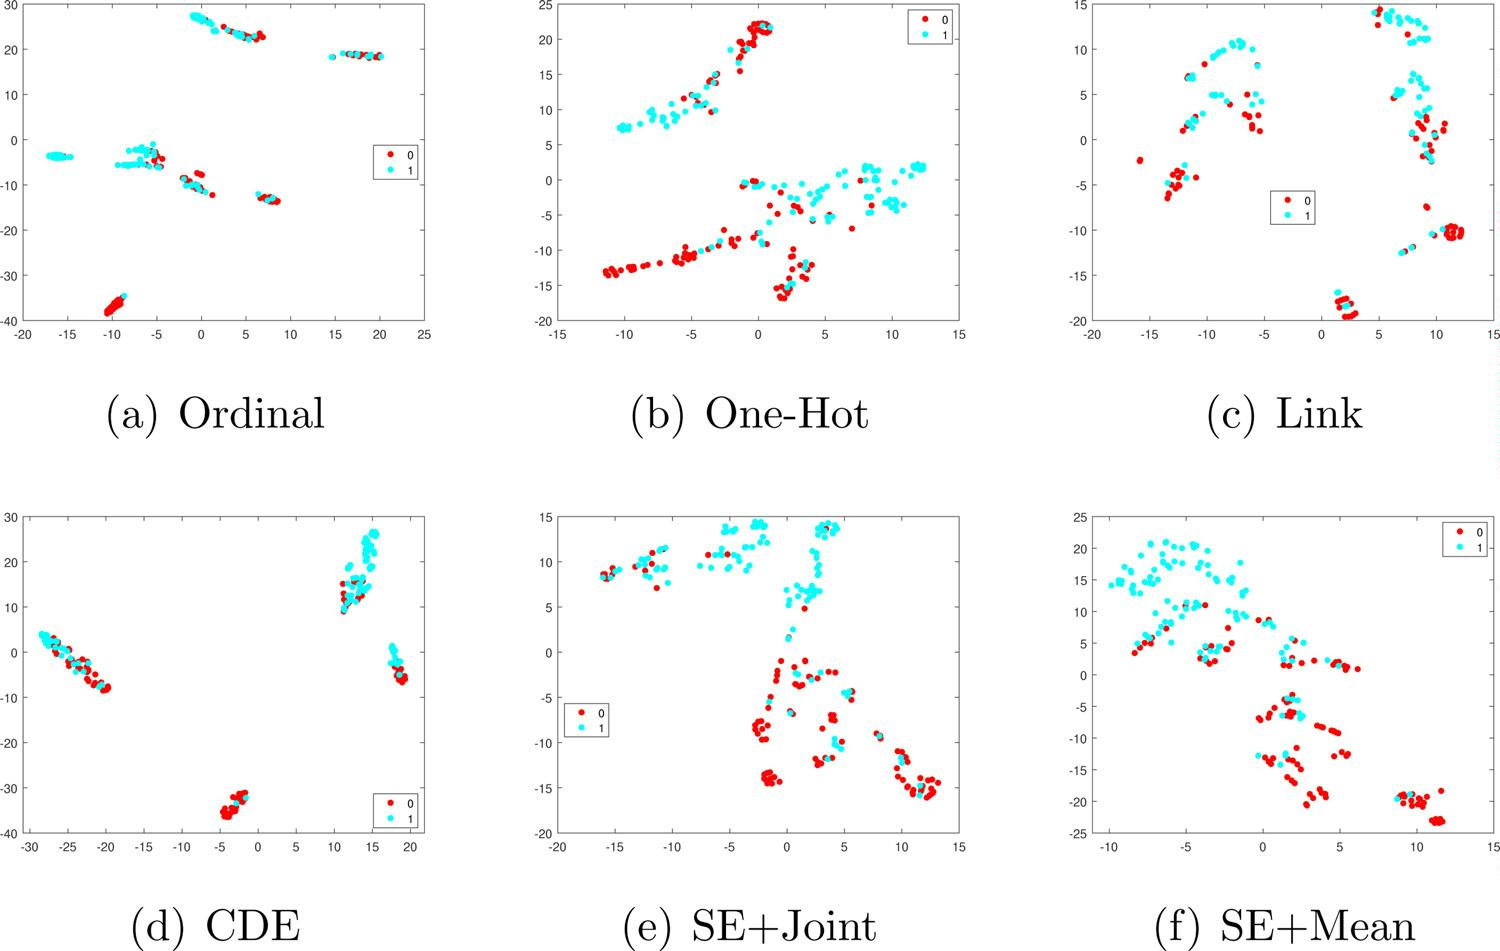
\includegraphics[width=360pt,height=228.12pt]{latexImage_e1b76af44ed903f870206f1ec6adcddd.png}}
\put(193.767,-288.837){\fontsize{6.3761}{1}\usefont{T1}{cmr}{b}{n}\selectfont\color{color_29791}F}
\put(102.624,-546.084){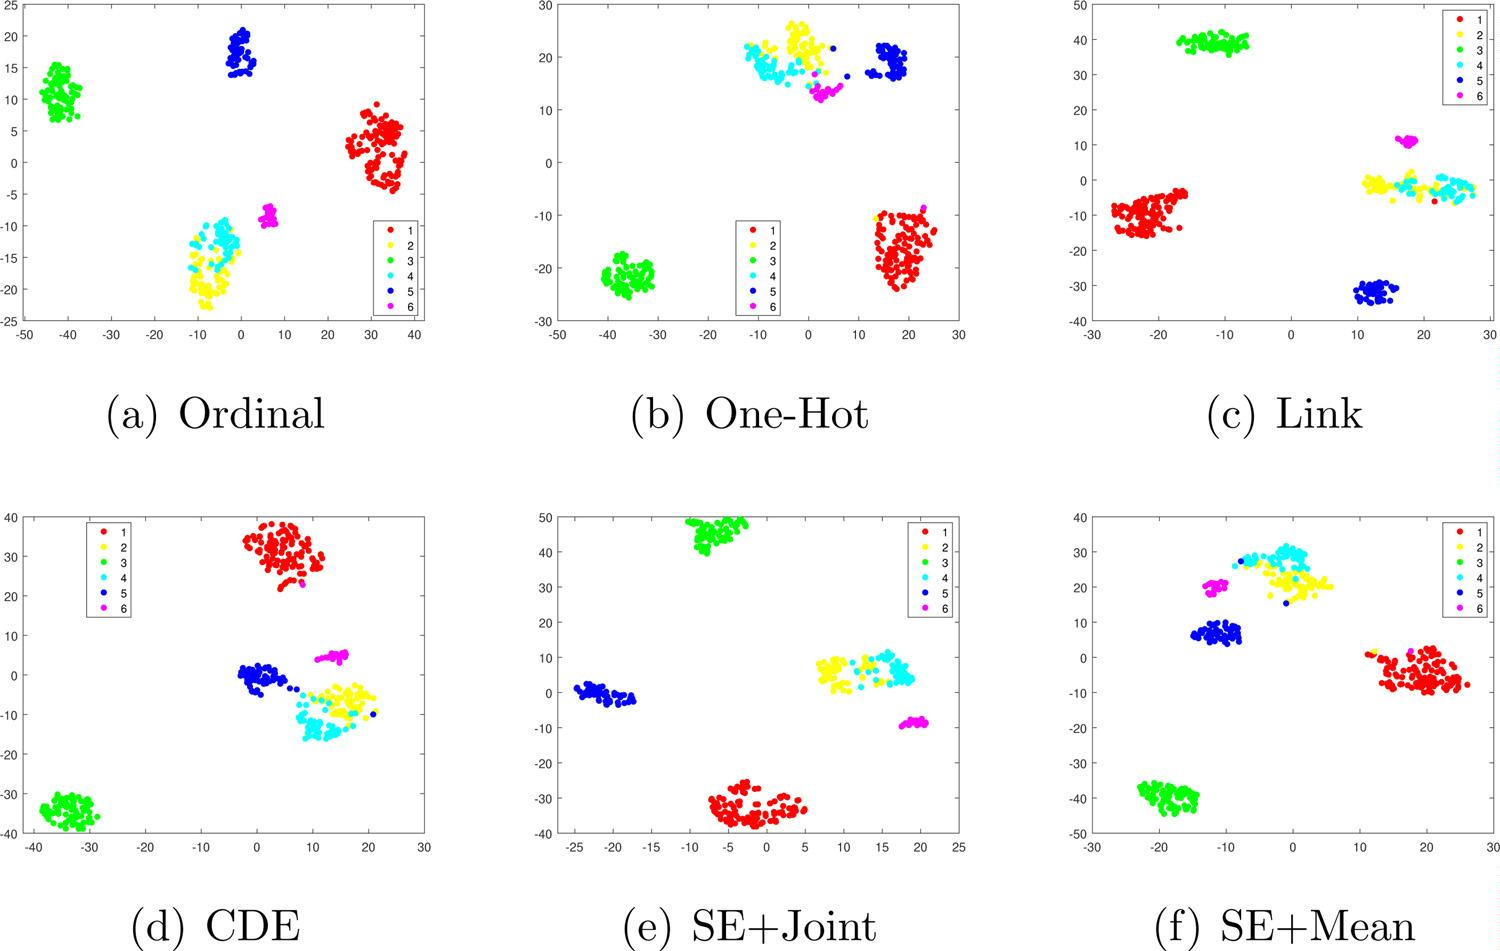
\includegraphics[width=360pt,height=228.12pt]{latexImage_dd2b6f1943caf5b68cd7f7aa065cbca2.png}}
\put(195.261,-560.628){\fontsize{6.3761}{1}\usefont{T1}{cmr}{b}{n}\selectfont\color{color_29791}Fig. 7. Scatter plots of different methods on Dermatology. }
\put(22.605,-596.547){\fontsize{7.9701}{1}\usefont{T1}{cmr}{m}{n}\selectfont\color{color_29791}measure the clustering accuracy, we employ two widely-used in- }
\put(22.605,-607.0049){\fontsize{7.9701}{1}\usefont{T1}{cmr}{m}{n}\selectfont\color{color_29791}dices, i.e., the normalized mutual information (NMI) and the ad- }
\put(22.605,-617.4719){\fontsize{7.9701}{1}\usefont{T1}{cmr}{m}{n}\selectfont\color{color_29791}justed rand index (ARI) [36] which measure the similarity between }
\put(22.605,-627.9299){\fontsize{7.9701}{1}\usefont{T1}{cmr}{m}{n}\selectfont\color{color_29791}a clustering result and the true partition on a data set. If a cluster- }
\put(22.605,-638.388){\fontsize{7.9701}{1}\usefont{T1}{cmr}{m}{n}\selectfont\color{color_29791}ing result is close to the true partition, then its NMI and ARI val- }
\put(22.605,-648.8549){\fontsize{7.9701}{1}\usefont{T1}{cmr}{m}{n}\selectfont\color{color_29791}ues are high. We record the mean and standard deviation of ARI }
\put(22.605,-659.313){\fontsize{7.9701}{1}\usefont{T1}{cmr}{m}{n}\selectfont\color{color_29791}and NMI of each method on each data set. Besides, we count the }
\put(22.605,-669.771){\fontsize{7.9701}{1}\usefont{T1}{cmr}{m}{n}\selectfont\color{color_29791}running time (seconds) of each compared algorithm in the task of }
\put(22.605,-680.238){\fontsize{7.9701}{1}\usefont{T1}{cmr}{m}{n}\selectfont\color{color_29791}converting categorical data. }
\put(22.605,-702.036){\fontsize{7.9701}{1}\usefont{T1}{cmr}{m}{n}\selectfont\color{color_29791}3.2. Clustering accuracy }
\put(34.557,-722.961){\fontsize{7.9701}{1}\usefont{T1}{cmr}{m}{n}\selectfont\color{color_33931}Table 4 shows the clustering performance of different graph }
\put(22.605,-733.4189){\fontsize{7.9701}{1}\usefont{T1}{cmr}{m}{n}\selectfont\color{color_29791}embedding and integration methods in the proposed framework }
\put(291.597,-596.547){\fontsize{7.9701}{1}\usefont{T1}{cmr}{m}{n}\selectfont\color{color_29791}on given eight categorical data sets. In this table, we also calcu- }
\put(291.597,-607.0049){\fontsize{7.9701}{1}\usefont{T1}{cmr}{m}{n}\selectfont\color{color_29791}late their average and maximum values on each data set. Accord- }
\put(291.597,-617.4719){\fontsize{7.9701}{1}\usefont{T1}{cmr}{m}{n}\selectfont\color{color_29791}ing to the table, we can see that the performance of the pro- }
\put(291.597,-627.9299){\fontsize{7.9701}{1}\usefont{T1}{cmr}{m}{n}\selectfont\color{color_29791}posed framework based on the mean operation is similar to the }
\put(291.597,-638.388){\fontsize{7.9701}{1}\usefont{T1}{cmr}{m}{n}\selectfont\color{color_29791}joint operation. However, the computation cost of the mean op- }
\put(291.597,-648.8549){\fontsize{7.9701}{1}\usefont{T1}{cmr}{m}{n}\selectfont\color{color_29791}eration is obviously less than the joint operation. The main rea- }
\put(291.597,-659.313){\fontsize{7.9701}{1}\usefont{T1}{cmr}{m}{n}\selectfont\color{color_29791}son is the Matlab environment is more suitable for the mean op- }
\put(291.597,-669.771){\fontsize{7.9701}{1}\usefont{T1}{cmr}{m}{n}\selectfont\color{color_29791}eration. Thus, we need to further optimize the code of the joint }
\put(291.597,-680.238){\fontsize{7.9701}{1}\usefont{T1}{cmr}{m}{n}\selectfont\color{color_29791}operation. Besides, the joint operation easily makes each of con- }
\put(291.597,-690.696){\fontsize{7.9701}{1}\usefont{T1}{cmr}{m}{n}\selectfont\color{color_29791}verted data become a high-dimensional data, which further adds }
\put(291.597,-701.154){\fontsize{7.9701}{1}\usefont{T1}{cmr}{m}{n}\selectfont\color{color_29791}the computation costs. In Table 4 , we also can observe that the ef- }
\put(291.597,-711.621){\fontsize{7.9701}{1}\usefont{T1}{cmr}{m}{n}\selectfont\color{color_29791}fect of the different graph embedding methods on the clustering }
\put(291.597,-722.0789){\fontsize{7.9701}{1}\usefont{T1}{cmr}{m}{n}\selectfont\color{color_29791}performance. We found that the quality of the converted categor- }
\put(291.597,-732.537){\fontsize{7.9701}{1}\usefont{T1}{cmr}{m}{n}\selectfont\color{color_29791}ical data based on non graph embedding is not worse than that }
\put(280.779,-754.344){\fontsize{6.3761}{1}\usefont{T1}{cmr}{m}{n}\selectfont\color{color_29791}6 }
\end{picture}
\newpage
\begin{tikzpicture}[overlay]\path(0pt,0pt);\end{tikzpicture}
\begin{picture}(-5,0)(2.5,0)
\put(22.605,-31.13098){\fontsize{6.3761}{1}\usefont{T1}{cmr}{m}{n}\selectfont\color{color_29791}L.}
\put(102.624,-274.293){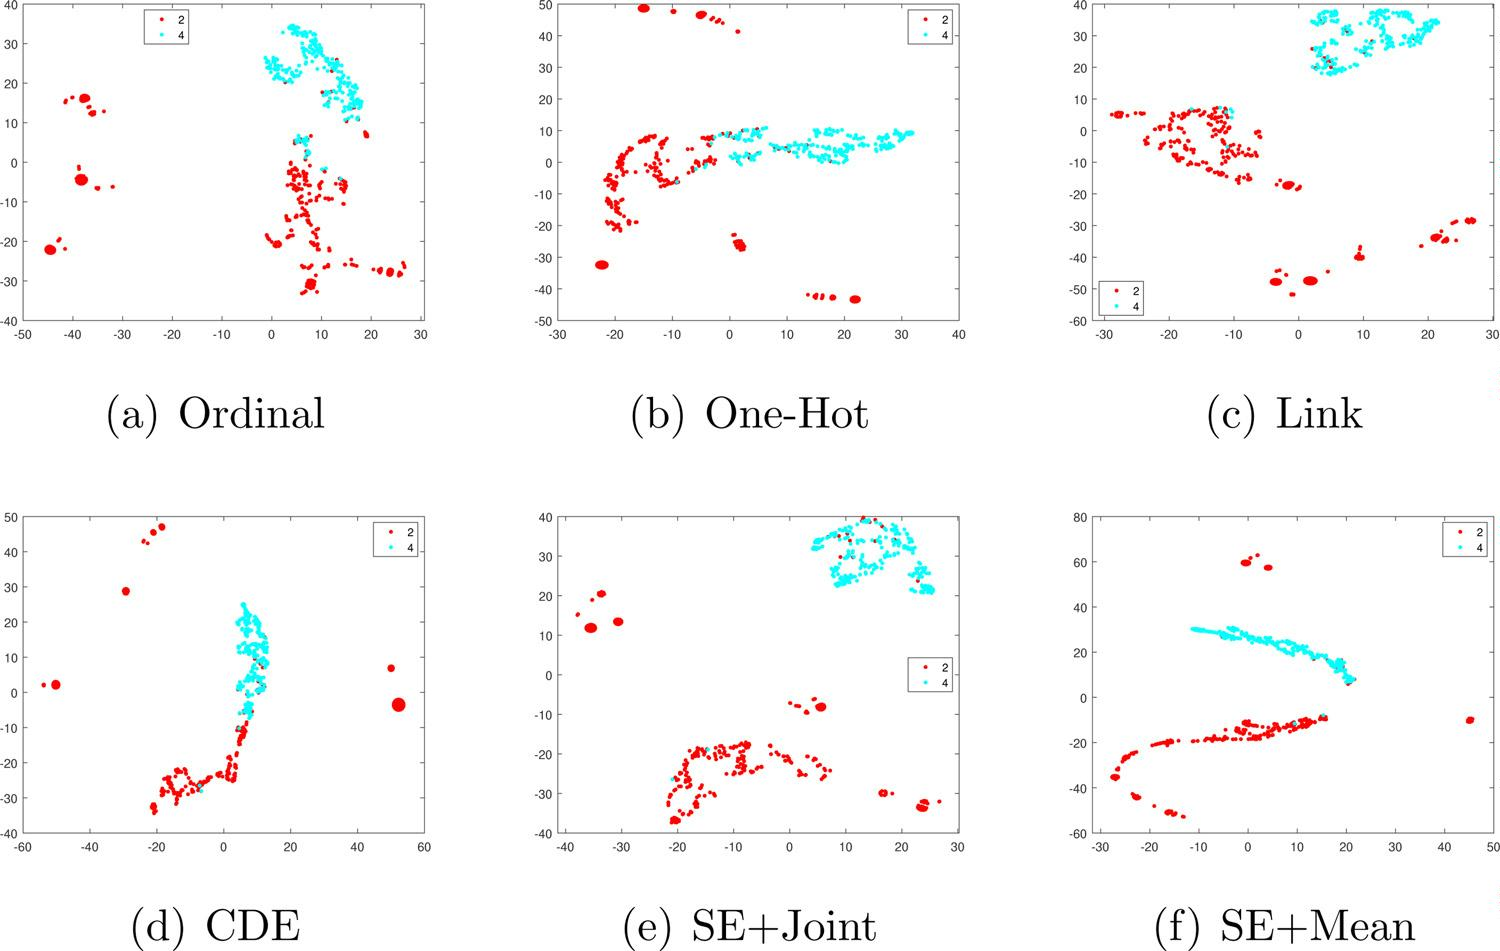
\includegraphics[width=360pt,height=228.12pt]{latexImage_10d972162bce1899ded8651ceff62081.png}}
\put(194.127,-288.837){\fontsize{6.3761}{1}\usefont{T1}{cmr}{b}{n}\selectfont\color{color_29791}F}
\put(102.624,-544.086){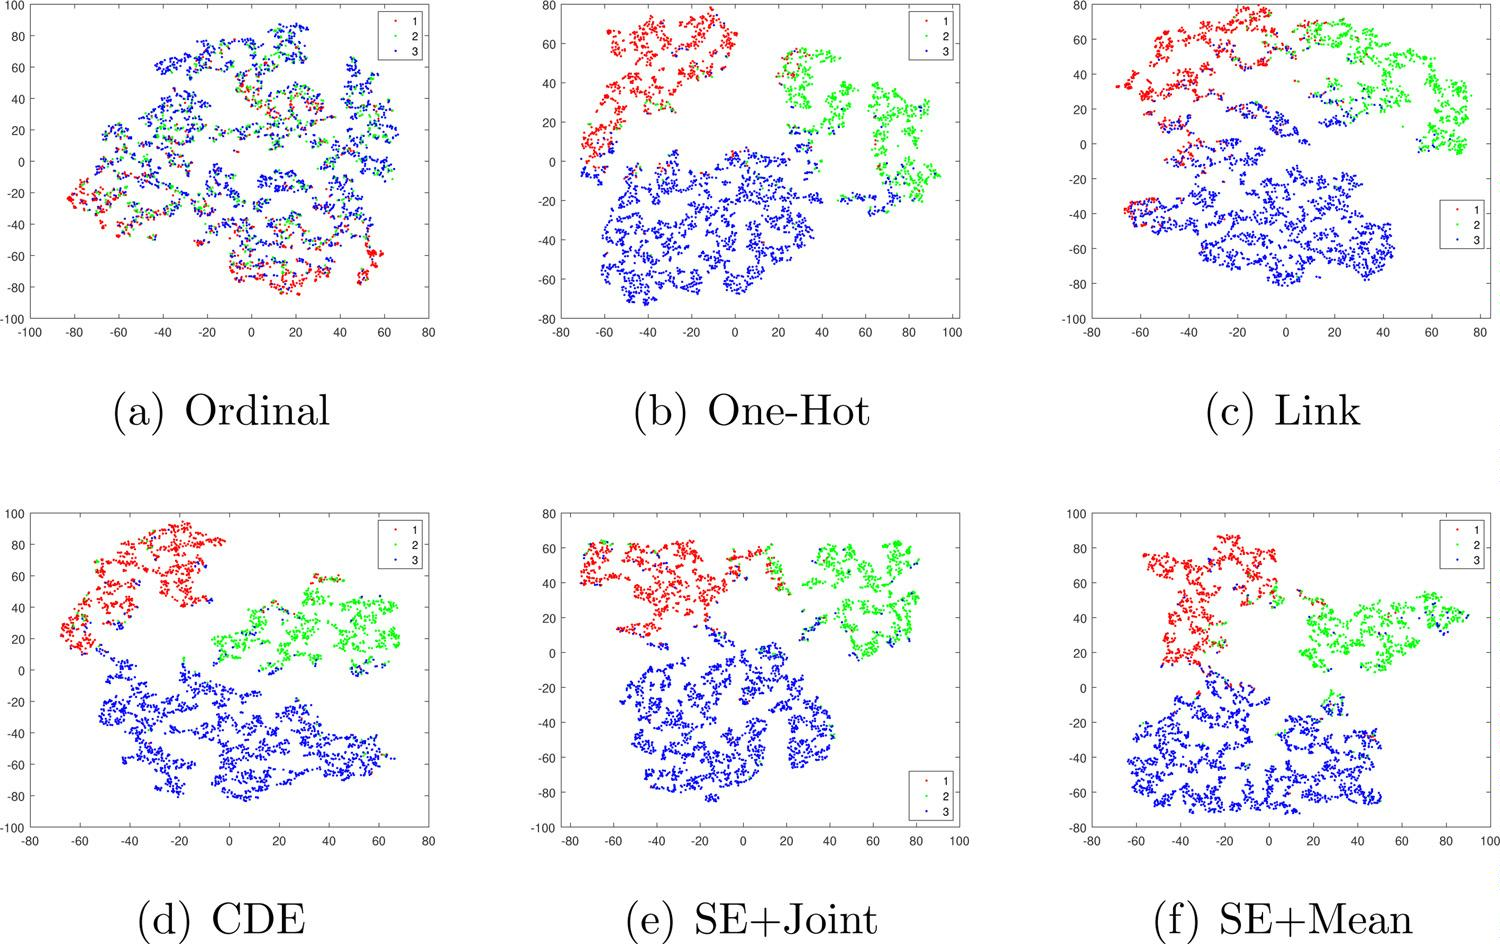
\includegraphics[width=360pt,height=226.44pt]{latexImage_f09f587a6b6418b8633949dce227d5fe.png}}
\put(207.177,-558.6299){\fontsize{6.3761}{1}\usefont{T1}{cmr}{b}{n}\selectfont\color{color_29791}Fig. 9. Scatter plots of different methods on DNA. }
\put(22.605,-602.5229){\fontsize{7.9701}{1}\usefont{T1}{cmr}{m}{n}\selectfont\color{color_29791}based on graph embedding. However, the non graph embedding }
\put(22.605,-612.981){\fontsize{7.9701}{1}\usefont{T1}{cmr}{m}{n}\selectfont\color{color_29791}method needs high computational costs, due to the high dimen- }
\put(22.605,-623.4389){\fontsize{7.9701}{1}\usefont{T1}{cmr}{m}{n}\selectfont\color{color_29791}sionality of the converted categorical data. }
\put(34.557,-633.8969){\fontsize{7.9701}{1}\usefont{T1}{cmr}{m}{n}\selectfont\color{color_29791}Furthermore, we compare the proposed framework based on }
\put(22.605,-644.364){\fontsize{7.9701}{1}\usefont{T1}{cmr}{m}{n}\selectfont\color{color_29791}spectral embedding (CDC\_DR+SE) with other algorithms. We first }
\put(22.605,-654.8219){\fontsize{7.9701}{1}\usefont{T1}{cmr}{m}{n}\selectfont\color{color_29791}show the visual results of categorical data encoding methods on }
\put(22.605,-665.2799){\fontsize{7.9701}{1}\usefont{T1}{cmr}{m}{n}\selectfont\color{color_29791}different data sets, which can be seen in Figs. 4–11 . These visual }
\put(22.605,-675.7469){\fontsize{7.9701}{1}\usefont{T1}{cmr}{m}{n}\selectfont\color{color_29791}results were produced by using t-SNE [41] to map the encoded cat- }
\put(22.605,-686.2049){\fontsize{7.9701}{1}\usefont{T1}{cmr}{m}{n}\selectfont\color{color_29791}egorical data into 2-dimensional spaces. According to these figures, }
\put(22.605,-696.663){\fontsize{7.9701}{1}\usefont{T1}{cmr}{m}{n}\selectfont\color{color_29791}we can see that the visual results of CDC\_DR+SE are better than }
\put(22.605,-707.1299){\fontsize{7.9701}{1}\usefont{T1}{cmr}{m}{n}\selectfont\color{color_29791}other algorithms on most of data sets. We also can observe that }
\put(22.605,-717.588){\fontsize{7.9701}{1}\usefont{T1}{cmr}{m}{n}\selectfont\color{color_29791}the visual results of CDC\_DR+SE with the joint operation are supe- }
\put(22.605,-728.046){\fontsize{7.9701}{1}\usefont{T1}{cmr}{m}{n}\selectfont\color{color_29791}rior to the mean operation. However, since the information loss is }
\put(291.597,-602.5229){\fontsize{7.9701}{1}\usefont{T1}{cmr}{m}{n}\selectfont\color{color_29791}caused by reducing dimensions, the performance of an algorithm }
\put(291.597,-612.981){\fontsize{7.9701}{1}\usefont{T1}{cmr}{m}{n}\selectfont\color{color_29791}can not be effectively evaluated in some cases. For example, on }
\put(291.597,-623.4389){\fontsize{7.9701}{1}\usefont{T1}{cmr}{m}{n}\selectfont\color{color_29791}data set mushroom, we can not judge which algorithm is effective. }
\put(291.597,-633.8969){\fontsize{7.9701}{1}\usefont{T1}{cmr}{m}{n}\selectfont\color{color_29791}Therefore, we need to further compare the clustering accuracy of }
\put(291.597,-644.364){\fontsize{7.9701}{1}\usefont{T1}{cmr}{m}{n}\selectfont\color{color_29791}different algorithms, which can be seen in Table 5 . According to }
\put(291.597,-654.8219){\fontsize{7.9701}{1}\usefont{T1}{cmr}{m}{n}\selectfont\color{color_33931}Table 5 , we can observe that the clustering accuracy of the pro- }
\put(291.597,-665.2799){\fontsize{7.9701}{1}\usefont{T1}{cmr}{m}{n}\selectfont\color{color_29791}posed framework is better than other algorithms on most of the }
\put(291.597,-675.7469){\fontsize{7.9701}{1}\usefont{T1}{cmr}{m}{n}\selectfont\color{color_29791}tested data sets. The comparison results show that the proposed }
\put(291.597,-686.2049){\fontsize{7.9701}{1}\usefont{T1}{cmr}{m}{n}\selectfont\color{color_29791}framework can obtain an appropriate representation for clustering }
\put(291.597,-696.663){\fontsize{7.9701}{1}\usefont{T1}{cmr}{m}{n}\selectfont\color{color_29791}categorical data in most cases. According to Tables 4 and 5 , we also }
\put(291.597,-707.1299){\fontsize{7.9701}{1}\usefont{T1}{cmr}{m}{n}\selectfont\color{color_29791}can observe that the maximum ARI and NMI values of the pro- }
\put(291.597,-717.588){\fontsize{7.9701}{1}\usefont{T1}{cmr}{m}{n}\selectfont\color{color_29791}posed framework with different graph embeddings in Table 4 are }
\put(291.597,-728.046){\fontsize{7.9701}{1}\usefont{T1}{cmr}{m}{n}\selectfont\color{color_29791}obviously superior to other algorithms in Table 5 on all the tested }
\put(280.779,-754.344){\fontsize{6.3761}{1}\usefont{T1}{cmr}{m}{n}\selectfont\color{color_29791}7 }
\end{picture}
\newpage
\begin{tikzpicture}[overlay]\path(0pt,0pt);\end{tikzpicture}
\begin{picture}(-5,0)(2.5,0)
\put(22.605,-31.13098){\fontsize{6.3761}{1}\usefont{T1}{cmr}{m}{n}\selectfont\color{color_29791}L.}
\put(102.624,-274.293){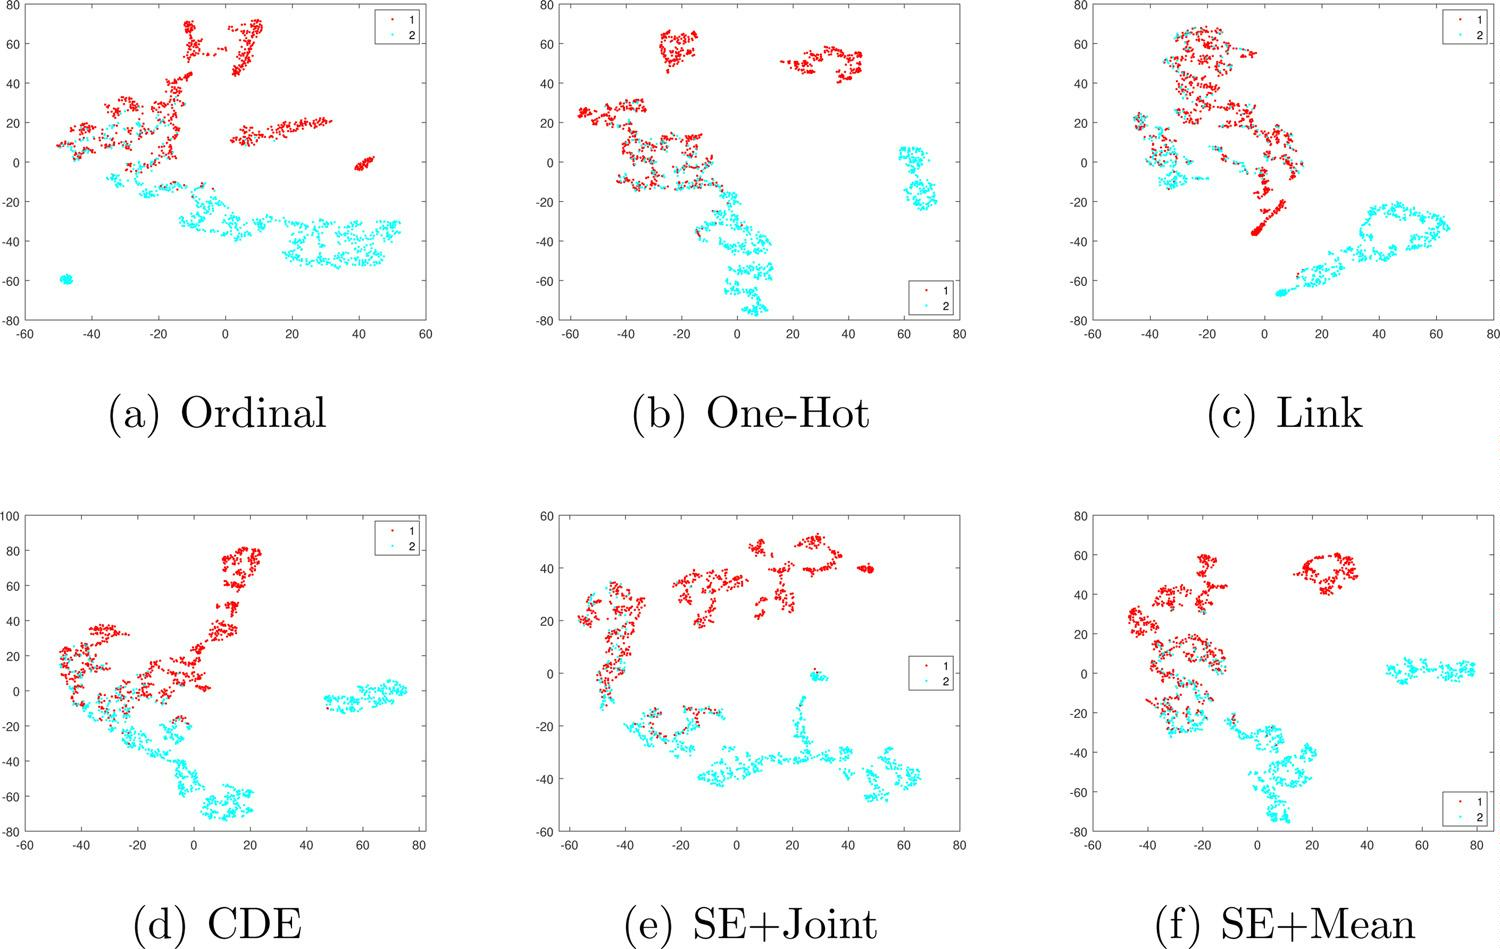
\includegraphics[width=360pt,height=227.76pt]{latexImage_2438f376a7f85116ccc48ac533f3cec5.png}}
\put(202.245,-288.837){\fontsize{6.3761}{1}\usefont{T1}{cmr}{b}{n}\selectfont\color{color_29791}F}
\put(102.624,-544.086){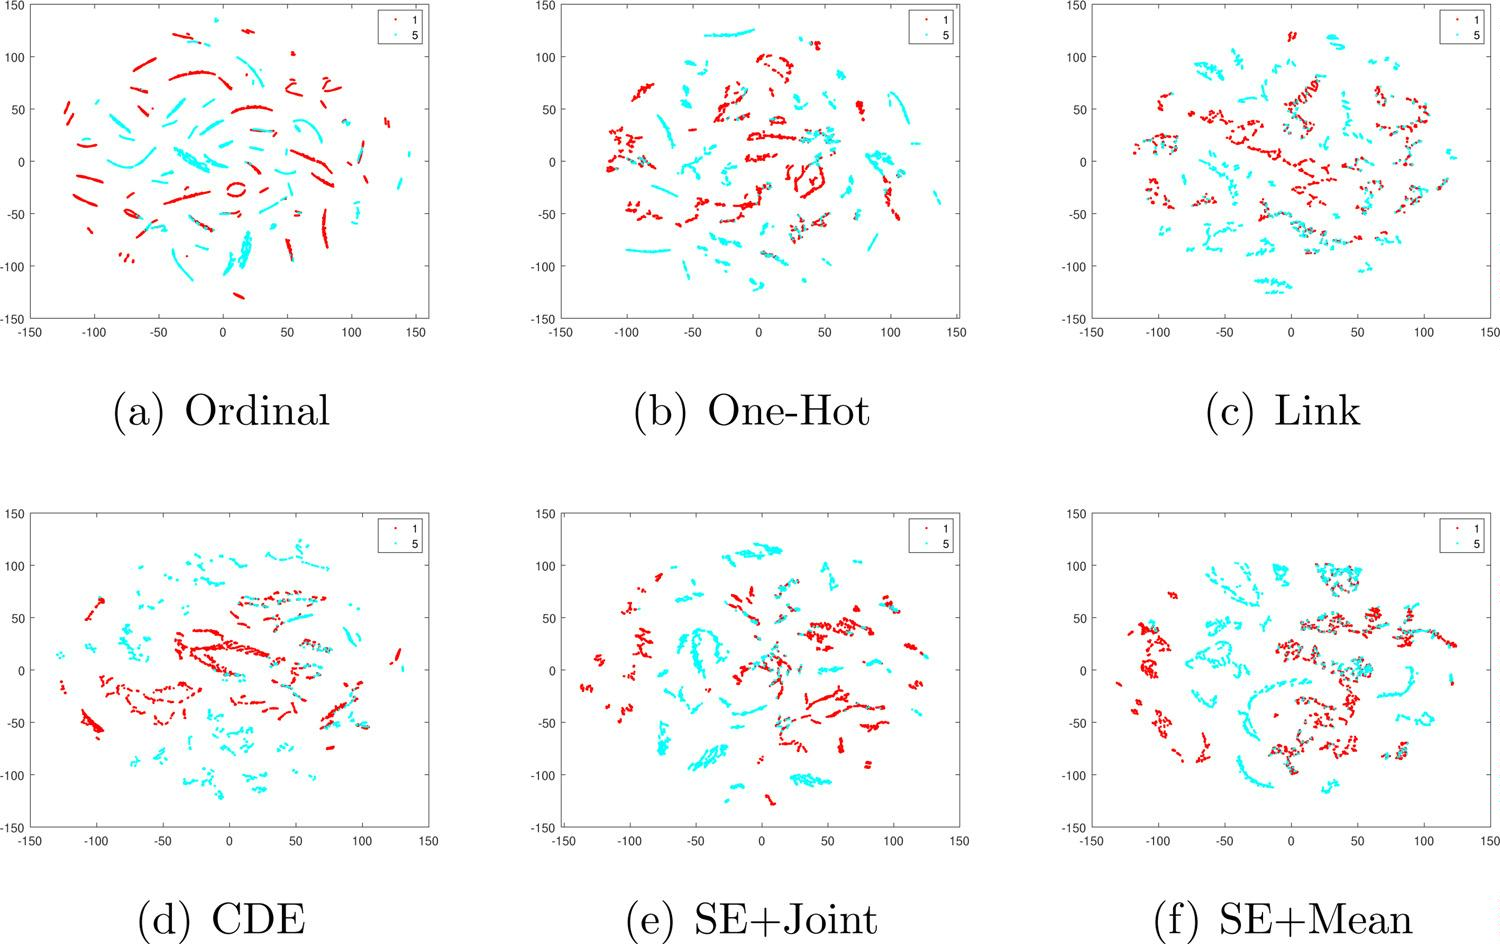
\includegraphics[width=360pt,height=226.44pt]{latexImage_459bef2c6a112a98bad735409464c340.png}}
\put(196.467,-558.6299){\fontsize{6.3761}{1}\usefont{T1}{cmr}{b}{n}\selectfont\color{color_29791}Fig. 11. Scatter plots of different methods on Mushroom. }
\put(22.605,-594.549){\fontsize{7.9701}{1}\usefont{T1}{cmr}{m}{n}\selectfont\color{color_29791}data sets. This indicates that if we can select an appropriate graph }
\put(22.605,-605.0069){\fontsize{7.9701}{1}\usefont{T1}{cmr}{m}{n}\selectfont\color{color_29791}embedding or integration method, a good representation of cate- }
\put(22.605,-615.474){\fontsize{7.9701}{1}\usefont{T1}{cmr}{m}{n}\selectfont\color{color_29791}gorical data can be obtained. }
\put(34.557,-625.9319){\fontsize{7.9701}{1}\usefont{T1}{cmr}{m}{n}\selectfont\color{color_29791}Besides, in the experiment, we test the clustering performance }
\put(22.605,-636.3899){\fontsize{7.9701}{1}\usefont{T1}{cmr}{m}{n}\selectfont\color{color_29791}of the proposed framework on clustering ensemble. We run k - }
\put(22.605,-646.848){\fontsize{7.9701}{1}\usefont{T1}{cmr}{m}{n}\selectfont\color{color_29791}means 60 times on each of given numerical data sets to get its cat- }
\put(22.605,-657.3149){\fontsize{7.9701}{1}\usefont{T1}{cmr}{m}{n}\selectfont\color{color_29791}egorical data. In order to make the categorical features as different }
\put(22.605,-667.773){\fontsize{7.9701}{1}\usefont{T1}{cmr}{m}{n}\selectfont\color{color_29791}as possible, we set different initial parameters in each time. We }
\put(22.605,-678.231){\fontsize{7.9701}{1}\usefont{T1}{cmr}{m}{n}\selectfont\color{color_29791}randomly select the number of clusters from the interval [ k/ 2 , 2 k ] }
\put(22.605,-688.698){\fontsize{7.9701}{1}\usefont{T1}{cmr}{m}{n}\selectfont\color{color_29791}and the corresponding initial seeds from a data set. We test the }
\put(22.605,-699.156){\fontsize{7.9701}{1}\usefont{T1}{cmr}{m}{n}\selectfont\color{color_29791}proposed framework with different graph embedding and integra- }
\put(22.605,-709.614){\fontsize{7.9701}{1}\usefont{T1}{cmr}{m}{n}\selectfont\color{color_29791}tion methods on the clustering ensemble tasks of given five data }
\put(22.605,-720.081){\fontsize{7.9701}{1}\usefont{T1}{cmr}{m}{n}\selectfont\color{color_29791}sets. The testing results are shown in Table 6 . Furthermore, we se- }
\put(22.605,-730.539){\fontsize{7.9701}{1}\usefont{T1}{cmr}{m}{n}\selectfont\color{color_29791}lect the proposed algorithm with spectral embedding to compare it }
\put(291.597,-594.549){\fontsize{7.9701}{1}\usefont{T1}{cmr}{m}{n}\selectfont\color{color_29791}with other algorithms, which is shown in Table 7 . In the tables, the }
\put(291.597,-605.0069){\fontsize{7.9701}{1}\usefont{T1}{cmr}{m}{n}\selectfont\color{color_29791}bold ARI and NMI values are higher than the best values of other }
\put(291.597,-615.474){\fontsize{7.9701}{1}\usefont{T1}{cmr}{m}{n}\selectfont\color{color_29791}compared algorithms. According to Tables 6 and 7 , we can see that }
\put(291.597,-625.9319){\fontsize{7.9701}{1}\usefont{T1}{cmr}{m}{n}\selectfont\color{color_29791}the categorical data converted by the proposed framework can fur- }
\put(291.597,-636.3899){\fontsize{7.9701}{1}\usefont{T1}{cmr}{m}{n}\selectfont\color{color_29791}ther enhance the performance of clustering ensemble. }
\put(291.597,-660.1949){\fontsize{7.9701}{1}\usefont{T1}{cmr}{m}{n}\selectfont\color{color_29791}3.3. Clustering efiiciency }
\put(303.549,-681.111){\fontsize{7.9701}{1}\usefont{T1}{cmr}{m}{n}\selectfont\color{color_33931}Table 8 shows the time costs (seconds) for converting categor- }
\put(291.597,-691.578){\fontsize{7.9701}{1}\usefont{T1}{cmr}{m}{n}\selectfont\color{color_29791}ical data of each algorithm. We can see that the converting costs }
\put(291.597,-702.036){\fontsize{7.9701}{1}\usefont{T1}{cmr}{m}{n}\selectfont\color{color_29791}of k -modes, ordinal encoding and one-hot encoding are very low, }
\put(291.597,-712.494){\fontsize{7.9701}{1}\usefont{T1}{cmr}{m}{n}\selectfont\color{color_29791}since they need not learn the representation of categorical data. }
\put(291.597,-722.961){\fontsize{7.9701}{1}\usefont{T1}{cmr}{m}{n}\selectfont\color{color_29791}For some algorithms, e.g., Link, CDE and the proposed framework }
\put(291.597,-733.4189){\fontsize{7.9701}{1}\usefont{T1}{cmr}{m}{n}\selectfont\color{color_29791}with NMF, their converting costs are very high on the tasks of clus- }
\put(280.779,-754.344){\fontsize{6.3761}{1}\usefont{T1}{cmr}{m}{n}\selectfont\color{color_29791}8 }
\end{picture}
\newpage
\begin{tikzpicture}[overlay]\path(0pt,0pt);\end{tikzpicture}
\begin{picture}(-5,0)(2.5,0)
\put(22.605,-31.13098){\fontsize{6.3761}{1}\usefont{T1}{cmr}{m}{n}\selectfont\color{color_29791}L. Bai and J. Liang Pattern Recognition 128 (2022) 108694 }
\put(25.59475,-51.34515){\fontsize{6.3761}{1}\usefont{T1}{cmr}{b}{n}\selectfont\color{color_29791}Table 5 }
\put(25.59475,-59.91333){\fontsize{6.3761}{1}\usefont{T1}{cmr}{m}{n}\selectfont\color{color_29791}Different methods for clustering categorical data. }
\put(31.569,-74.03387){\fontsize{6.3761}{1}\usefont{T1}{cmr}{m}{n}\selectfont\color{color_29791}Dataset Index KModes Ordinal One-Hot Link CDE CDC\_DR + SE }
\put(426.093,-87.29102){\fontsize{6.3761}{1}\usefont{T1}{cmr}{m}{n}\selectfont\color{color_29791}Joint Mean }
\put(31.614,-100.683){\fontsize{6.3761}{1}\usefont{T1}{cmr}{m}{n}\selectfont\color{color_29791}Soybean ARI 0.6340 ±0.17 0.6756 ±0.16 0.7263 ±0.2 0.6892 ±0.19 0.7297 ±0.19 0.7498 ±0.2 0.8572 ±0.19 }
\put(91.3944,-109.2512){\fontsize{6.3761}{1}\usefont{T1}{cmr}{m}{n}\selectfont\color{color_29791}NMI 0.7681 ±0.12 0.8075 ±0.1 0.8460 ±0.11 0.8238 ±0.12 0.8458 ±0.12 0.8627 ±0.11 0.9254 ±0.1 }
\put(31.61846,-117.8194){\fontsize{6.3761}{1}\usefont{T1}{cmr}{m}{n}\selectfont\color{color_29791}Zoo ARI 0.6447 ±0.14 0.6461 ±0.16 0.6393 ±0.14 0.654 ±0.13 0.6285}
\put(386.7777,-117.819){\fontsize{6.3761}{1}\usefont{T1}{cmr}{m}{n}\selectfont\color{color_29791} ±0.16 0.6414 ±0.14 0.6623 ±0.14 }
\put(91.39212,-126.3872){\fontsize{6.3761}{1}\usefont{T1}{cmr}{m}{n}\selectfont\color{color_29791}NMI 0.7552 ±0.06 0.7620 ±0.07 0.7603 ±0.06 0.7554 ±0.07 0.7625 ±0.07 0.7777 ±0.07 0.7823 ±0.06 }
\put(31.61618,-134.9554){\fontsize{6.3761}{1}\usefont{T1}{cmr}{m}{n}\selectfont\color{color_29791}Heart ARI 0.2816 ±0.13 0.2204 ±0.14 0.3784 ±0.11 0.0703 ±0.11 0.2398 ±0.15 0.4232 ±0.06 0.4208 ±0.00 }
\put(31.61809,-143.5147){\fontsize{6.3761}{1}\usefont{T1}{cmr}{m}{n}\selectfont\color{color_29791}disease NMI 0.2297 ±0.1 0.1755 }
\put(207.4862,-143.514){\fontsize{6.3761}{1}\usefont{T1}{cmr}{m}{n}\selectfont\color{color_29791}±0.11 0.2988 ±0.09 0.0688 ±0.08 0.1918 ±0.11 0.3342 ±0.05 0.3297 ±0.00 }
\put(31.61487,-152.0822){\fontsize{6.3761}{1}\usefont{T1}{cmr}{m}{n}\selectfont\color{color_29791}Derm- ARI 0.4295 ±0.12 0.6568 ±0.13 0.652 ±0.17 0.5995 ±0.18 0.6207 ±0.16 0.6887 ±0.16 0.5449 ±0.09 }
\put(31.61678,-160.6504){\fontsize{6.3761}{1}\usefont{T1}{cmr}{m}{n}\selectfont\color{color_29791}atology NMI 0.5609 ±0.1 0.8147 ±0.06 0.8007 ±0.09 0.7609 ±0.11 0.7814 ±0.08 0.8183 ±0.08 }
\put(485.8903,-160.65){\fontsize{6.3761}{1}\usefont{T1}{cmr}{m}{n}\selectfont\color{color_29791}0.7279 ±0.03 }
\put(31.61358,-169.2182){\fontsize{6.3761}{1}\usefont{T1}{cmr}{m}{n}\selectfont\color{color_29791}Breast ARI 0.5655 ±0.3 0.8335 ±0.01 0.796 ±0.00 0.8825 ±0.00 0.8714 ±0.02 0.8988 ±0.00 0.9043 ±0.00 }
\put(31.61358,-177.7864){\fontsize{6.3761}{1}\usefont{T1}{cmr}{m}{n}\selectfont\color{color_29791}cancer NMI 0.4973 ±0.23 0.7293 ±0.01 0.7227 ±0.00 0.8038 ±0.00 0.7953 ±0.02 0.8269 ±0.00 0.8377 ±0.00 }
\put(31.61485,-186.3546){\fontsize{6.3761}{1}\usefont{T1}{cmr}{m}{n}\selectfont\color{color_29791}DNA ARI 0.0183 ±0.01 0.0395 ±0.02 0.4759 ±0.11}
\put(285.1441,-186.3539){\fontsize{6.3761}{1}\usefont{T1}{cmr}{m}{n}\selectfont\color{color_29791} 0.3348 ±0.21 0.6172 ±0.12 0.5077 ±0.12 0.6799 ±0.13 }
\put(91.39291,-194.9221){\fontsize{6.3761}{1}\usefont{T1}{cmr}{m}{n}\selectfont\color{color_29791}NMI 0.0314 ±0.02 0.0435 ±0.02 0.4529 ±0.08 0.3963 ±0.13 0.5728 ±0.10 0.4739 ±0.09 0.6344 ±0.11 }
\put(31.61697,-203.4903){\fontsize{6.3761}{1}\usefont{T1}{cmr}{m}{n}\selectfont\color{color_29791}Letters ARI 0.1649 ±0.09 0.4460 ±0.00 0.2798 ±0.28 0.1160 ±0.18 0.3315 ±0.25 0.4862 ±0.23 0.4404 ±0.19 }
\put(91.3961,-212.0585){\fontsize{6.3761}{1}\usefont{T1}{cmr}{m}{n}\selectfont\color{color_29791}NMI 0.1359 }
\put(147.7118,-212.058){\fontsize{6.3761}{1}\usefont{T1}{cmr}{m}{n}\selectfont\color{color_29791}±0.08 0.3665 ±0.00 0.2413 ±0.25 0.1122 ±0.17 0.3019 ±0.24 0.4641 ±0.21 0.4275 ±0.15 }
\put(31.61513,-220.6262){\fontsize{6.3761}{1}\usefont{T1}{cmr}{m}{n}\selectfont\color{color_29791}Mush- ARI 0.3391 ±0.24 0.1883 ±0.19 0.3895 ±0.25 0.1839 ±0.18 0.4515 ±0.23 0.6165 ±0.09 0.6070 ±0.09 }
\put(31.61705,-229.1944){\fontsize{6.3761}{1}\usefont{T1}{cmr}{m}{n}\selectfont\color{color_29791}room NMI 0.3179 ±0.23 0.1642 ±0.15 0.3871 ±0.21 0.2302 ±0.16 0.4469 ±0.18 }
\put(426.1238,-229.194){\fontsize{6.3761}{1}\usefont{T1}{cmr}{m}{n}\selectfont\color{color_29791}0.5845 ±0.08 0.5734 ±0.08 }
\put(25.593,-268.704){\fontsize{6.3761}{1}\usefont{T1}{cmr}{b}{n}\selectfont\color{color_29791}Table 6 }
\put(25.593,-277.2722){\fontsize{6.3761}{1}\usefont{T1}{cmr}{m}{n}\selectfont\color{color_29791}The proposed framework for clustering ensemble. }
\put(31.569,-291.393){\fontsize{6.3761}{1}\usefont{T1}{cmr}{m}{n}\selectfont\color{color_29791}Dataset Index NE SE NMF AE Average Max }
\put(95.694,-304.641){\fontsize{6.3761}{1}\usefont{T1}{cmr}{m}{n}\selectfont\color{color_29791}Joint Mean Joint Mean Joint Mean Joint Mean }
\put(31.614,-318.033){\fontsize{6.3761}{1}\usefont{T1}{cmr}{m}{n}\selectfont\color{color_29791}Iris ARI 0.5638 ±0.15 0.5907 ±0.12 0.663 ±0.11 0.6887 ±0.1 0.6344 ±0.14 0.6163 ±0.11 0.6753 ±0.12 0.7080 ±0.11 0.6425 ±0.12 0.7080 ±0.15 }
\put(69.66019,-326.6012){\fontsize{6.3761}{1}\usefont{T1}{cmr}{m}{n}\selectfont\color{color_29791}NMI 0.6787 ±0.11 0.7029 ±0.09 0.7401 ±0.06 0.7658 ±0.07 0.7399 ±0.08 0.7293 ±0.07 0.7262 ±0.08 0.7757 ±0.08 0.7323 ±0.08 }
\put(491.8691,-326.601){\fontsize{6.3761}{1}\usefont{T1}{cmr}{m}{n}\selectfont\color{color_29791}0.7757 ±0.11 }
\put(31.61351,-335.1692){\fontsize{6.3761}{1}\usefont{T1}{cmr}{m}{n}\selectfont\color{color_29791}Isolet ARI 0.5384 ±0.04 0.5305 ±0.04 0.5658 ±0.03 0.5408 ±0.05 0.5527 ±0.03 0.5437 ±0.04 0.5454 ±0.04 0.5612 ±0.03 0.5473 ±0.04 0.5658 ±0.05 }
\put(69.65842,-343.7374){\fontsize{6.3761}{1}\usefont{T1}{cmr}{m}{n}\selectfont\color{color_29791}NMI 0.7727 ±0.01 0.7694 ±0.01 0.7908 ±0.01 0.7777 ±0.02 0.7822 ±0.01 0.7765 ±0.02 0.7898 ±0.01 0.7833 ±0.01 }
\put(447.8525,-343.737){\fontsize{6.3761}{1}\usefont{T1}{cmr}{m}{n}\selectfont\color{color_29791}0.7803 ±0.01 0.7908 ±0.02 }
\put(31.61432,-352.3052){\fontsize{6.3761}{1}\usefont{T1}{cmr}{m}{n}\selectfont\color{color_29791}COIL20 ARI 0.5918 ±0.05 0.579 ±0.06 0.608 ±0.05 0.5779 ±0.06 0.5995 ±0.04 0.5899 ±0.05 0.6021 ±0.05 0.6121 ±0.04 0.5950 ±0.05 0.6121 ±0.06 }
\put(69.66114,-360.8734){\fontsize{6.3761}{1}\usefont{T1}{cmr}{m}{n}\selectfont\color{color_29791}NMI 0.8052 ±0.02 0.8052 ±0.02 0.8146 ±0.02 0.8062 ±0.02 0.8126 ±0.02 0.8124 ±0.02 0.8113 ±0.02 }
\put(403.836,-360.873){\fontsize{6.3761}{1}\usefont{T1}{cmr}{m}{n}\selectfont\color{color_29791}0.8126 ±0.02 0.8100 ±0.02 0.8146 ±0.02 }
\put(31.61458,-369.4412){\fontsize{6.3761}{1}\usefont{T1}{cmr}{m}{n}\selectfont\color{color_29791}Optical- ARI 0.6797 ±0.09 0.6838 ±0.11 0.7307 ±0.08 0.7285 ±0.07 0.7097 ±0.08 0.7081 ±0.07 0.6929 ±0.09 0.7253 ±0.06 0.7073 ±0.08 0.7307 ±0.11 }
\put(31.61841,-378.0094){\fontsize{6.3761}{1}\usefont{T1}{cmr}{m}{n}\selectfont\color{color_29791}Digits NMI 0.8024 ±0.04 0.8051 ±0.04 0.8248 ±0.03 0.8198 ±0.03 0.8212 ±0.03 0.8173 ±}
\put(341.2881,-378.009){\fontsize{6.3761}{1}\usefont{T1}{cmr}{m}{n}\selectfont\color{color_29791}0.03 0.806 ±0.04 0.8193 ±0.03 0.8145 ±0.03 0.8248 ±0.04 }
\put(31.61431,-386.5772){\fontsize{6.3761}{1}\usefont{T1}{cmr}{m}{n}\selectfont\color{color_29791}Pen- ARI 0.5408 ±0.06 0.5565 ±0.06 0.5621 ±0.04 0.5481 ±0.05 0.5538 ±0.04 0.5412 ±0.05 0.545 ±0.04 0.5763 ±0.05 0.553 ±0.05 0.5763 ±0.06 }
\put(31.6175,-395.1454){\fontsize{6.3761}{1}\usefont{T1}{cmr}{m}{n}\selectfont\color{color_29791}Digits NMI 0.6979 ±0.03 0.705 ±0.03 0.7015 ±0.02 0.6923 ±0.03 0.6955}
\put(292.2233,-395.145){\fontsize{6.3761}{1}\usefont{T1}{cmr}{m}{n}\selectfont\color{color_29791} ±0.02 0.6911 ±0.03 0.6959 ±0.02 0.7098 ±0.02 0.6986 ±0.02 0.7098 ±0.03 }
\put(25.593,-434.646){\fontsize{6.3761}{1}\usefont{T1}{cmr}{b}{n}\selectfont\color{color_29791}Table 7 }
\put(25.593,-443.2142){\fontsize{6.3761}{1}\usefont{T1}{cmr}{m}{n}\selectfont\color{color_29791}Different methods for clustering ensemble. }
\put(31.569,-457.335){\fontsize{6.3761}{1}\usefont{T1}{cmr}{m}{n}\selectfont\color{color_29791}Dataset Index }
\put(118.248,-455.022){\fontsize{4.4632}{1}\usefont{T1}{cmr}{m}{n}\selectfont\color{color_29791}∗}
\put(121.065,-457.335){\fontsize{6.3761}{1}\usefont{T1}{cmr}{m}{n}\selectfont\color{color_29791}KModes Ordinal One-Hot Link CDE CDC\_DR + SE }
\put(424.599,-470.583){\fontsize{6.3761}{1}\usefont{T1}{cmr}{m}{n}\selectfont\color{color_29791}Joint Mean }
\put(31.614,-483.9749){\fontsize{6.3761}{1}\usefont{T1}{cmr}{m}{n}\selectfont\color{color_29791}Iris ARI 0.5664 ±0.15 0.5991 ±0.14 0.5464 ±0.17 0.6087 ±0.10 0.5594 ±0.14 0.6630 ±0.11 0.6887 ±0.10 }
\put(80.92676,-492.5431){\fontsize{6.3761}{1}\usefont{T1}{cmr}{m}{n}\selectfont\color{color_29791}NMI 0.6799 ±0.12 0.6715 ±0.11 0.6547 ±0.14 0.7251 ±0.05 0.6618 ±0.11 0.7401 ±0.06 0.7658 ±0.07 }
\put(31.61783,-501.1113){\fontsize{6.3761}{1}\usefont{T1}{cmr}{m}{n}\selectfont\color{color_29791}Isolet ARI 0.5323 ±0.03 0.5034 ±0.03 0.5277 ±0.04 0.5465 ±0.04 0.5325}
\put(383.7893,-501.111){\fontsize{6.3761}{1}\usefont{T1}{cmr}{m}{n}\selectfont\color{color_29791} ±0.04 0.5658 ±0.03 0.5408 ±0.05 }
\put(80.92519,-509.6792){\fontsize{6.3761}{1}\usefont{T1}{cmr}{m}{n}\selectfont\color{color_29791}NMI 0.7596 ±0.01 0.7414 ±0.01 0.7623 ±0.01 0.7788 ±0.01 0.7667 ±0.01 0.7908 ±0.01 0.7777 ±0.02 }
\put(31.61626,-518.2474){\fontsize{6.3761}{1}\usefont{T1}{cmr}{m}{n}\selectfont\color{color_29791}COIL20 ARI 0.5859 ±0.04 0.5858 ±0.05 0.5826 ±0.05 0.5923 ±0.04 0.5862 ±0.05 0.6080 ±0.05 0.5779 ±0.06 }
\put(80.92965,-526.8156){\fontsize{6.3761}{1}\usefont{T1}{cmr}{m}{n}\selectfont\color{color_29791}NMI 0.7904 ±0.02 0.7970 ±0.02}
\put(217.8814,-526.8149){\fontsize{6.3761}{1}\usefont{T1}{cmr}{m}{n}\selectfont\color{color_29791} 0.7962 ±0.02 0.8055 ±0.02 0.8012 ±0.02 0.8146 ±0.02 0.8062 ±0.02 }
\put(31.61448,-535.3831){\fontsize{6.3761}{1}\usefont{T1}{cmr}{m}{n}\selectfont\color{color_29791}Optical- ARI 0.6840 ±0.09 0.6537 ±0.10 0.6563 ±0.10 0.6859 ±0.10 0.6467 ±0.08 0.7307 ±0.08 0.7285 ±0.07 }
\put(31.61639,-543.9513){\fontsize{6.3761}{1}\usefont{T1}{cmr}{m}{n}\selectfont\color{color_29791}Digits NMI 0.7930 ±0.04 0.7767 ±0.05 0.792 ±0.04 0.8033 ±0.04 0.7852 ±0.03 0.8248 ±0.03 0.8198 }
\put(506.3462,-543.951){\fontsize{6.3761}{1}\usefont{T1}{cmr}{m}{n}\selectfont\color{color_29791}±0.03 }
\put(31.61304,-552.5192){\fontsize{6.3761}{1}\usefont{T1}{cmr}{m}{n}\selectfont\color{color_29791}Pen- ARI 0.5363 ±0.05 0.5439 ±0.06 0.5493 ±0.06 0.5548 ±0.05 0.5495 ±0.07 0.5621 ±0.04 0.5481 ±0.05 }
\put(31.61495,-561.0874){\fontsize{6.3761}{1}\usefont{T1}{cmr}{m}{n}\selectfont\color{color_29791}Digits NMI 0.6793 ±0.03 0.6898 ±0.03 0.7006 ±0.03 0.7063 ±0.02 0.7011 ±0.03 0.7015 ±0.02 0.6923 ±0.03 }
\put(22.605,-614.169){\fontsize{7.9701}{1}\usefont{T1}{cmr}{m}{n}\selectfont\color{color_29791}tering ensemble. The main reason is that their computational com- }
\put(22.605,-624.6269){\fontsize{7.9701}{1}\usefont{T1}{cmr}{m}{n}\selectfont\color{color_29791}plexity is related to the number of the categorical values. In the }
\put(22.605,-635.0939){\fontsize{7.9701}{1}\usefont{T1}{cmr}{m}{n}\selectfont\color{color_29791}clustering ensemble, if the number of clusters on a data set is not a }
\put(22.605,-645.5519){\fontsize{7.9701}{1}\usefont{T1}{cmr}{m}{n}\selectfont\color{color_29791}small value, the number of the produced categorical values is very }
\put(22.605,-656.0099){\fontsize{7.9701}{1}\usefont{T1}{cmr}{m}{n}\selectfont\color{color_29791}large. We can observe that the converting costs of the proposed }
\put(22.605,-666.4769){\fontsize{7.9701}{1}\usefont{T1}{cmr}{m}{n}\selectfont\color{color_29791}framework based on the joint operation are higher than the mean }
\put(22.605,-676.9349){\fontsize{7.9701}{1}\usefont{T1}{cmr}{m}{n}\selectfont\color{color_29791}operation, since the dimensions of the encoded objects based on }
\put(22.605,-687.393){\fontsize{7.9701}{1}\usefont{T1}{cmr}{m}{n}\selectfont\color{color_29791}the joint operation are very high, compared to the mean operation. }
\put(22.605,-697.8599){\fontsize{7.9701}{1}\usefont{T1}{cmr}{m}{n}\selectfont\color{color_29791}For example, since NE does not implement the graph embedding, }
\put(22.605,-708.318){\fontsize{7.9701}{1}\usefont{T1}{cmr}{m}{n}\selectfont\color{color_29791}the number of the dimensions of the encoded data based on NE }
\put(22.605,-718.776){\fontsize{7.9701}{1}\usefont{T1}{cmr}{m}{n}\selectfont\color{color_29791}and joint is very large. Thus, we can see that its computational }
\put(22.605,-729.243){\fontsize{7.9701}{1}\usefont{T1}{cmr}{m}{n}\selectfont\color{color_29791}costs are very high, compared to the proposed framework with }
\put(291.597,-614.169){\fontsize{7.9701}{1}\usefont{T1}{cmr}{m}{n}\selectfont\color{color_29791}other graph embedding and operations. For the proposed frame- }
\put(291.597,-624.6269){\fontsize{7.9701}{1}\usefont{T1}{cmr}{m}{n}\selectfont\color{color_29791}work with AE, its converting cost is from training the weights of }
\put(291.597,-635.0939){\fontsize{7.9701}{1}\usefont{T1}{cmr}{m}{n}\selectfont\color{color_29791}the neural network. According to the above the analysis, we can }
\put(291.597,-645.5519){\fontsize{7.9701}{1}\usefont{T1}{cmr}{m}{n}\selectfont\color{color_29791}see that the propose framework with spectral embedding is a good }
\put(291.597,-656.0099){\fontsize{7.9701}{1}\usefont{T1}{cmr}{m}{n}\selectfont\color{color_29791}choice to convert categorical data into numerical data. It is very }
\put(291.597,-666.4769){\fontsize{7.9701}{1}\usefont{T1}{cmr}{m}{n}\selectfont\color{color_29791}efiicient, compared to other methods, except k -modes, ordinal en- }
\put(291.597,-676.9349){\fontsize{7.9701}{1}\usefont{T1}{cmr}{m}{n}\selectfont\color{color_29791}coding and one-hot encoding. }
\put(291.597,-702.036){\fontsize{7.9701}{1}\usefont{T1}{cmr}{b}{n}\selectfont\color{color_29791}4. Conclusions }
\put(303.549,-722.961){\fontsize{7.9701}{1}\usefont{T1}{cmr}{m}{n}\selectfont\color{color_29791}In this paper, we have proposed a simple categorical data clus- }
\put(291.597,-733.4189){\fontsize{7.9701}{1}\usefont{T1}{cmr}{m}{n}\selectfont\color{color_29791}tering framework based on data representation. In this framework, }
\put(280.779,-754.344){\fontsize{6.3761}{1}\usefont{T1}{cmr}{m}{n}\selectfont\color{color_29791}9 }
\end{picture}
\begin{tikzpicture}[overlay]
\path(0pt,0pt);
\draw[color_29791,line width=0.504pt]
(25.593pt, -65.19598pt) -- (539.673pt, -65.19598pt)
;
\draw[color_29791,line width=0.504pt]
(426.093pt, -78.948pt) -- (533.697pt, -78.948pt)
;
\draw[color_29791,line width=0.504pt]
(25.59299pt, -91.836pt) -- (539.673pt, -91.836pt)
;
\draw[color_29791,line width=0.504pt]
(25.59299pt, -234.504pt) -- (539.673pt, -234.504pt)
;
\draw[color_29791,line width=0.504pt]
(25.59299pt, -282.546pt) -- (539.673pt, -282.546pt)
;
\draw[color_29791,line width=0.504pt]
(95.69398pt, -296.298pt) -- (181.554pt, -296.298pt)
;
\draw[color_29791,line width=0.504pt]
(183.723pt, -296.298pt) -- (269.583pt, -296.298pt)
;
\draw[color_29791,line width=0.504pt]
(271.761pt, -296.298pt) -- (357.621pt, -296.298pt)
;
\draw[color_29791,line width=0.504pt]
(359.79pt, -296.298pt) -- (445.65pt, -296.298pt)
;
\draw[color_29791,line width=0.504pt]
(447.828pt, -296.298pt) -- (489.678pt, -296.298pt)
;
\draw[color_29791,line width=0.504pt]
(491.847pt, -296.298pt) -- (533.697pt, -296.298pt)
;
\draw[color_29791,line width=0.504pt]
(25.59299pt, -309.195pt) -- (539.673pt, -309.195pt)
;
\draw[color_29791,line width=0.504pt]
(25.59299pt, -400.446pt) -- (539.673pt, -400.446pt)
;
\draw[color_29791,line width=0.504pt]
(25.59299pt, -448.497pt) -- (539.673pt, -448.497pt)
;
\draw[color_29791,line width=0.504pt]
(424.599pt, -462.2401pt) -- (533.697pt, -462.2401pt)
;
\draw[color_29791,line width=0.504pt]
(25.59299pt, -475.1371pt) -- (539.673pt, -475.1371pt)
;
\draw[color_29791,line width=0.504pt]
(25.59299pt, -566.3971pt) -- (539.673pt, -566.3971pt)
;
\end{tikzpicture}
\newpage
\begin{tikzpicture}[overlay]\path(0pt,0pt);\end{tikzpicture}
\begin{picture}(-5,0)(2.5,0)
\put(22.605,-31.13098){\fontsize{6.3761}{1}\usefont{T1}{cmr}{m}{n}\selectfont\color{color_29791}L. Bai and J. Liang Pattern Recognition 128 (2022) 108694 }
\put(22.60691,-51.34515){\fontsize{6.3761}{1}\usefont{T1}{cmr}{b}{n}\selectfont\color{color_29791}Table 8 }
\put(22.60691,-59.91333){\fontsize{6.3761}{1}\usefont{T1}{cmr}{m}{n}\selectfont\color{color_29791}Running time of different methods in the task of converting categorical data. }
\put(28.581,-74.03387){\fontsize{6.3761}{1}\usefont{T1}{cmr}{m}{n}\selectfont\color{color_29791}Dataset KModes Ordinal One-Hot Link CDE NE SE NMF AE }
\put(255.363,-87.29102){\fontsize{6.3761}{1}\usefont{T1}{cmr}{m}{n}\selectfont\color{color_29791}Joint Mean Joint Mean Joint Mean Joint Mean }
\put(28.626,-100.683){\fontsize{6.3761}{1}\usefont{T1}{cmr}{m}{n}\selectfont\color{color_29791}Soybean 0.0000 0.0010 0.0034 0.0058 0.1166 0.0038 0.0013 0.0038 0.0026 0.0191 0.0180 4.6984 7.0965 }
\put(28.62919,-109.2512){\fontsize{6.3761}{1}\usefont{T1}{cmr}{m}{n}\selectfont\color{color_29791}Zoo 0.0000 0.0005 0.0029 0.0037 0.0653 0.0055 0.0017 0.0072 0.0025 0.0212 0.0203 1.6663 1.1171 }
\put(28.63301,-117.8194){\fontsize{6.3761}{1}\usefont{T1}{cmr}{m}{n}\selectfont\color{color_29791}Heart disease 0.0000 0.0005 0.0029 0.0048 0.0389 0.0084 0.0024 0.0056 0.0026 0.0140 0.0118 0.3443 0.3226 }
\put(28.63748,-126.3876){\fontsize{6.3761}{1}\usefont{T1}{cmr}{m}{n}\selectfont\color{color_29791}Dermatology 0.0000 0.0012 0.0086 0.0329 0.5235 0.1679 0.0104}
\put(311.2149,-126.387){\fontsize{6.3761}{1}\usefont{T1}{cmr}{m}{n}\selectfont\color{color_29791} 0.0328 0.0195 0.1500 0.1290 6.5814 6.4826 }
\put(28.62679,-134.9552){\fontsize{6.3761}{1}\usefont{T1}{cmr}{m}{n}\selectfont\color{color_29791}Breast cancer 0.0000 0.0007 0.0050 0.0269 0.2378 0.0998 0.0067 0.0183 0.0101 0.0306 0.0213 1.4607 3.3474 }
\put(28.63061,-143.5145){\fontsize{6.3761}{1}\usefont{T1}{cmr}{m}{n}\selectfont\color{color_29791}DNA 0.0000 0.0154 0.1314 1.5587 6.3501 65.6748 0.1712 32.7012 0.2118 0.9341 0.3218 19.0252 21.8677 }
\put(28.63061,-152.0827){\fontsize{6.3761}{1}\usefont{T1}{cmr}{m}{n}\selectfont\color{color_29791}Letters 0.0000 0.0024 0.0181 0.2174 1.0808 2.0595 0.0316 0.1558 0.0545 0.2085 0.1608 1.3955 0.9997 }
\put(28.6338,-160.6509){\fontsize{6.3761}{1}\usefont{T1}{cmr}{m}{n}\selectfont\color{color_29791}Mushroom }
\put(78.376,-160.65){\fontsize{6.3761}{1}\usefont{T1}{cmr}{m}{n}\selectfont\color{color_29791}0.0000 0.0124 0.1187 1.8680 1.6209 67.2370 0.1529 1.8635 0.1623 0.9470 0.1733 10.4491 0.9844 }
\put(28.6252,-169.2182){\fontsize{6.3761}{1}\usefont{T1}{cmr}{m}{n}\selectfont\color{color_29791}Iris 0.0000 0.0023 0.0083 0.0965 2.5432 0.2051 0.0146 0.0724 0.0617 0.3634 0.3418 6.2808 5.6386 }
\put(28.62712,-177.7864){\fontsize{6.3761}{1}\usefont{T1}{cmr}{m}{n}\selectfont\color{color_29791}Isolet 0.0000 0.0127 0.0725 21.2449 286.2975 150.1505 0.4932 2.1724 1.1184 167.7374 162.8827 56.9398 65.7873 }
\put(28.62775,-186.3546){\fontsize{6.3761}{1}\usefont{T1}{cmr}{m}{n}\selectfont\color{color_29791}COIL20 0.0000 0.0100 0.0653 13.5457 174.5346 105.9927 0.3413 1.4001 0.7124}
\put(382.0423,-186.3539){\fontsize{6.3761}{1}\usefont{T1}{cmr}{m}{n}\selectfont\color{color_29791} 89.3360 85.1458 51.5457 93.7984 }
\put(28.62528,-194.9221){\fontsize{6.3761}{1}\usefont{T1}{cmr}{m}{n}\selectfont\color{color_29791}OpticalDigits 0.0000 0.0346 0.2479 21.8576 49.6414 598.5708 0.5865 6.3924 0.5893 20.4497 14.4980 22.3863 20.3012 }
\put(28.62464,-203.4903){\fontsize{6.3761}{1}\usefont{T1}{cmr}{m}{n}\selectfont\color{color_29791}PenDigits 0.0000 0.0658 0.4844 66.0219 74.4511 2375.3709 1.2974 27.7077 1.2774 41.0335 14.8203 40.0813 21.2100 }
\put(22.605,-236.646){\fontsize{7.9701}{1}\usefont{T1}{cmr}{m}{n}\selectfont\color{color_29791}we learn the representation of each categorical value by graph em- }
\put(22.605,-247.113){\fontsize{7.9701}{1}\usefont{T1}{cmr}{m}{n}\selectfont\color{color_29791}bedding and integrate the represented categorical values of a data }
\put(22.605,-257.571){\fontsize{7.9701}{1}\usefont{T1}{cmr}{m}{n}\selectfont\color{color_29791}object to convert it into numerical data. Since the proposed frame- }
\put(22.605,-268.029){\fontsize{7.9701}{1}\usefont{T1}{cmr}{m}{n}\selectfont\color{color_29791}work fully considers the relation between categorical values, it can }
\put(22.605,-278.496){\fontsize{7.9701}{1}\usefont{T1}{cmr}{m}{n}\selectfont\color{color_29791}help existing numerical clustering algorithms to cluster categorical }
\put(22.605,-288.9539){\fontsize{7.9701}{1}\usefont{T1}{cmr}{m}{n}\selectfont\color{color_29791}data and find out its potential and meaningful cluster structure. In }
\put(22.605,-299.412){\fontsize{7.9701}{1}\usefont{T1}{cmr}{m}{n}\selectfont\color{color_29791}the experimental analysis, we have compared the proposed frame- }
\put(22.605,-309.879){\fontsize{7.9701}{1}\usefont{T1}{cmr}{m}{n}\selectfont\color{color_29791}work with other five representation methods of categorical data on }
\put(22.605,-320.337){\fontsize{7.9701}{1}\usefont{T1}{cmr}{m}{n}\selectfont\color{color_29791}13 benchmark data sets. The comparison results have illustrated }
\put(22.605,-330.795){\fontsize{7.9701}{1}\usefont{T1}{cmr}{m}{n}\selectfont\color{color_29791}that the proposed framework has very good performance. }
\put(34.557,-341.253){\fontsize{7.9701}{1}\usefont{T1}{cmr}{m}{n}\selectfont\color{color_29791}In the future work, we will consider more complex or advanced }
\put(22.605,-351.7199){\fontsize{7.9701}{1}\usefont{T1}{cmr}{m}{n}\selectfont\color{color_29791}similarity measures to construct the graph of categorical values. }
\put(22.605,-362.178){\fontsize{7.9701}{1}\usefont{T1}{cmr}{m}{n}\selectfont\color{color_29791}Besides, we will try more graph embedding methods to represent }
\put(22.605,-372.636){\fontsize{7.9701}{1}\usefont{T1}{cmr}{m}{n}\selectfont\color{color_29791}the categorical values. We will further analyze the effect of the }
\put(22.605,-383.103){\fontsize{7.9701}{1}\usefont{T1}{cmr}{m}{n}\selectfont\color{color_29791}similarity measures and graph embeddings on the effectiveness of }
\put(22.605,-393.5609){\fontsize{7.9701}{1}\usefont{T1}{cmr}{m}{n}\selectfont\color{color_29791}the proposed framework. }
\put(22.605,-418.0139){\fontsize{7.9701}{1}\usefont{T1}{cmr}{b}{n}\selectfont\color{color_29791}Declaration of Competing Interest }
\put(34.557,-438.9389){\fontsize{7.9701}{1}\usefont{T1}{cmr}{m}{n}\selectfont\color{color_29791}The authors declare that they have no known competing finan- }
\put(22.605,-449.397){\fontsize{7.9701}{1}\usefont{T1}{cmr}{m}{n}\selectfont\color{color_29791}cial interests or personal relationships that could have appeared to }
\put(22.605,-459.8549){\fontsize{7.9701}{1}\usefont{T1}{cmr}{m}{n}\selectfont\color{color_29791}influence the work reported in this paper. }
\put(22.605,-484.308){\fontsize{7.9701}{1}\usefont{T1}{cmr}{b}{n}\selectfont\color{color_29791}Acknowledgment }
\put(34.557,-505.2329){\fontsize{7.9701}{1}\usefont{T1}{cmr}{m}{n}\selectfont\color{color_29791}The authors are very grateful to the editors and reviewers }
\put(22.605,-515.691){\fontsize{7.9701}{1}\usefont{T1}{cmr}{m}{n}\selectfont\color{color_29791}for their valuable comments and suggestions. This work is sup- }
\put(22.605,-526.149){\fontsize{7.9701}{1}\usefont{T1}{cmr}{m}{n}\selectfont\color{color_29791}ported by National Key Research and Development Program of }
\put(22.605,-536.616){\fontsize{7.9701}{1}\usefont{T1}{cmr}{m}{n}\selectfont\color{color_33931}China (No. 2020AAA0106100 ), the National Natural Science Foun- }
\put(22.605,-547.0739){\fontsize{7.9701}{1}\usefont{T1}{cmr}{m}{n}\selectfont\color{color_33931}dation of China (No. 62022052 ), the Technology Research Develop- }
\put(22.605,-557.5319){\fontsize{7.9701}{1}\usefont{T1}{cmr}{m}{n}\selectfont\color{color_29791}ment Projects of Shanxi (No. 201901D211192). }
\put(22.605,-579.4919){\fontsize{7.9701}{1}\usefont{T1}{cmr}{b}{n}\selectfont\color{color_29791}References }
\put(26.295,-597.924){\fontsize{6.3761}{1}\usefont{T1}{cmr}{m}{n}\selectfont\color{color_29791}[1] A.K. Jain , Data clustering: 50 years beyond k-means, in: W. Daelemans, }
\put(38.07803,-605.8979){\fontsize{6.3761}{1}\usefont{T1}{cmr}{m}{n}\selectfont\color{color_33931}B. Goethals, K. Morik (Eds.), Machine Learning and Knowledge Discovery in }
\put(38.07803,-613.863){\fontsize{6.3761}{1}\usefont{T1}{cmr}{m}{n}\selectfont\color{color_33931}Databases, Springer Berlin Heidelberg, Berlin, Heidelberg, 2008, pp. 3–4 . }
\put(26.29883,-621.8369){\fontsize{6.3761}{1}\usefont{T1}{cmr}{m}{n}\selectfont\color{color_29791}[2] J. MacQueen , Some methods for classification and analysis of multivariate ob- }
\put(38.07867,-629.8109){\fontsize{6.3761}{1}\usefont{T1}{cmr}{m}{n}\selectfont\color{color_33931}servations, in: Proceedings of}
\put(129.304,-629.811){\fontsize{6.3761}{1}\usefont{T1}{cmr}{m}{n}\selectfont\color{color_33931} the Fifth Berkeley Symposium on Mathemat- }
\put(38.07731,-637.776){\fontsize{6.3761}{1}\usefont{T1}{cmr}{m}{n}\selectfont\color{color_33931}ical Statistics and Probability, University of California Press, Berkeley, 1967, }
\put(38.07795,-645.75){\fontsize{6.3761}{1}\usefont{T1}{cmr}{m}{n}\selectfont\color{color_33931}pp. 281–297 . }
\put(26.29747,-653.715){\fontsize{6.3761}{1}\usefont{T1}{cmr}{m}{n}\selectfont\color{color_29791}[3] A . Rodriguez , A . Laio , Clustering by fast search and find of density peaks, Sci- }
\put(38.07731,-661.689){\fontsize{6.3761}{1}\usefont{T1}{cmr}{m}{n}\selectfont\color{color_33931}ence 344 (6191) (2014) 14 92–14 96 . }
\put(26.2981,-669.654){\fontsize{6.3761}{1}\usefont{T1}{cmr}{m}{n}\selectfont\color{color_29791}[4] A.Y. Ng , M.I. Jordan , Y. Weiss , On spectral clustering: analysis and an algorithm, }
\put(38.07567,-677.6279){\fontsize{6.3761}{1}\usefont{T1}{cmr}{m}{n}\selectfont\color{color_33931}in: Advances in Neural Information Processing Systems, 2001, pp. 849–856 . }
\put(26.29583,-685.593){\fontsize{6.3761}{1}\usefont{T1}{cmr}{m}{n}\selectfont\color{color_29791}[5] X. Zhu , Y. Zhu , W. Zheng , Spectral rotation for deep one-step clustering, Pattern }
\put(38.07631,-693.567){\fontsize{6.3761}{1}\usefont{T1}{cmr}{m}{n}\selectfont\color{color_33931}Recognit. 105 (2020) 107175 . }
\put(26.29519,-701.5409){\fontsize{6.3761}{1}\usefont{T1}{cmr}{m}{n}\selectfont\color{color_29791}[6] L. Guo , Q.}
\put(70.3047,-701.541){\fontsize{6.3761}{1}\usefont{T1}{cmr}{m}{n}\selectfont\color{color_33931} Dai , Graph clustering via variational graph embedding, Pattern }
\put(38.07606,-709.506){\fontsize{6.3761}{1}\usefont{T1}{cmr}{m}{n}\selectfont\color{color_33931}Recognit. 122 (2022) 108334 . }
\put(26.29622,-717.48){\fontsize{6.3761}{1}\usefont{T1}{cmr}{m}{n}\selectfont\color{color_29791}[7] L. Romeo , E. Frontoni , A unified hierarchical XGBoost model for classifying }
\put(38.07989,-725.445){\fontsize{6.3761}{1}\usefont{T1}{cmr}{m}{n}\selectfont\color{color_33931}priorities for COVID-19 vaccination campaign, Pattern Recognit. 121 (2022) }
\put(38.07925,-733.4189){\fontsize{6.3761}{1}\usefont{T1}{cmr}{m}{n}\selectfont\color{color_33931}108197 . }
\put(295.287,-236.646){\fontsize{6.3761}{1}\usefont{T1}{cmr}{m}{n}\selectfont\color{color_29791}[8] A. Nazabal , P.M. Olmos , Z. Ghahramani , I. Valera , Handling incomplete hetero- }
\put(307.0688,-244.6199){\fontsize{6.3761}{1}\usefont{T1}{cmr}{m}{n}\selectfont\color{color_33931}geneous data using VAEs, Pattern Recognit. 107 (2020) 107501 . }
\put(295.2889,-252.585){\fontsize{6.3761}{1}\usefont{T1}{cmr}{m}{n}\selectfont\color{color_29791}[9] S.-K. Ng , R. Tawiah , G.J. McLachlan , Unsupervised pattern recognition of mixed }
\put(307.0713,-260.559){\fontsize{6.3761}{1}\usefont{T1}{cmr}{m}{n}\selectfont\color{color_33931}data structures with numerical and categorical features using a mixture re- }
\put(307.0675,-268.533){\fontsize{6.3761}{1}\usefont{T1}{cmr}{m}{n}\selectfont\color{color_33931}gression modelling framework, Pattern Recognit. 88 (2019) 261–271 . }
\put(292.0301,-276.498){\fontsize{6.3761}{1}\usefont{T1}{cmr}{m}{n}\selectfont\color{color_29791}[10] R. Kuo , Y. Zheng , T.P.Q. Nguyen , Metaheuristic-based possibilistic fuzzy k–}
\put(307.0694,-284.4719){\fontsize{6.3761}{1}\usefont{T1}{cmr}{m}{n}\selectfont\color{color_33931}modes algorithms for categorical data clustering, Inf. Sci. 557 (2021) 1–15 . }
\put(292.3017,-292.437){\fontsize{6.3761}{1}\usefont{T1}{cmr}{m}{n}\selectfont\color{color_29791}[11] L. Bai , J. Liang , Cluster validity functions for categorical data: a solution-space }
\put(307.0674,-300.4109){\fontsize{6.3761}{1}\usefont{T1}{cmr}{m}{n}\selectfont\color{color_33931}perspective, Data Min. Knowl. Discov. 29 (6) (2015) 1560–1597 . }
\put(291.9311,-308.376){\fontsize{6.3761}{1}\usefont{T1}{cmr}{m}{n}\selectfont\color{color_29791}[12] S. Guha , R. Rastogi , S. Kyuseok , Rock: a robust clustering algorithm for cate- }
\put(307.0693,-316.3499){\fontsize{6.3761}{1}\usefont{T1}{cmr}{m}{n}\selectfont\color{color_33931}gorical attributes, in: Proceedings of the Fifteenth International Conference on }
\put(307.068,-324.3239){\fontsize{6.3761}{1}\usefont{T1}{cmr}{m}{n}\selectfont\color{color_33931}Data Engineering, 23–26, Sydney, Australia, 1999, pp. 512–521 . }
\put(292.0038,-332.2889){\fontsize{6.3761}{1}\usefont{T1}{cmr}{m}{n}\selectfont\color{color_29791}[13] Z. Huang , }
\put(338.8827,-332.289){\fontsize{6.3761}{1}\usefont{T1}{cmr}{m}{n}\selectfont\color{color_33931}Extensions to the k-means algorithm for clustering large data sets }
\put(307.0685,-340.2629){\fontsize{6.3761}{1}\usefont{T1}{cmr}{m}{n}\selectfont\color{color_33931}with categorical values, Data Min. Knowl. Discov. 2 (3) (1998) 283–304 . }
\put(292.0573,-348.228){\fontsize{6.3761}{1}\usefont{T1}{cmr}{m}{n}\selectfont\color{color_29791}[14] M. Ng , M.J. Li , Z.X. Huang , Z. He , On the impact of dissimilarity measure in }
\put(307.0698,-356.2019){\fontsize{6.3761}{1}\usefont{T1}{cmr}{m}{n}\selectfont\color{color_33931}k -modes clustering algorithm, IEEE Trans. Pattern Anal. Mach.}
\put(500.0081,-356.202){\fontsize{6.3761}{1}\usefont{T1}{cmr}{m}{n}\selectfont\color{color_33931} Intell. 29 (3) }
\put(307.068,-364.167){\fontsize{6.3761}{1}\usefont{T1}{cmr}{m}{n}\selectfont\color{color_33931}(2007) 503–507 . }
\put(292.021,-372.141){\fontsize{6.3761}{1}\usefont{T1}{cmr}{m}{n}\selectfont\color{color_29791}[15] J. Huang , M. Ng , H. Rong , Z. Li , Automated variable weighting in k-means type }
\put(307.068,-380.1149){\fontsize{6.3761}{1}\usefont{T1}{cmr}{m}{n}\selectfont\color{color_33931}clustering, IEEE Trans. Pattern Anal. Mach. Intell. 27 (5) (2005) 657–668 . }
\put(292.0484,-388.08){\fontsize{6.3761}{1}\usefont{T1}{cmr}{m}{n}\selectfont\color{color_29791}[16] L. Bai , J. Liang , C. Dang , F. Cao , The impact of cluster representatives on the }
\put(307.0681,-396.054){\fontsize{6.3761}{1}\usefont{T1}{cmr}{m}{n}\selectfont\color{color_33931}convergence of the k-modes type clustering, IEEE Trans. Pattern Anal. Mach. }
\put(307.0674,-404.019){\fontsize{6.3761}{1}\usefont{T1}{cmr}{m}{n}\selectfont\color{color_33931}Intell. 35 (6) (2013) 1509–1522 . }
\put(292.2003,-411.9929){\fontsize{6.3761}{1}\usefont{T1}{cmr}{m}{n}\selectfont\color{color_29791}[17] Y. Xiao , C. Huang , J. Huang , I. Kaku , Y. Xu , Optimal mathematical programming }
\put(307.0687,-419.9579){\fontsize{6.3761}{1}\usefont{T1}{cmr}{m}{n}\selectfont\color{color_33931}and variable neighborhood search for k-modes categorical data}
\put(495.85,-419.958){\fontsize{6.3761}{1}\usefont{T1}{cmr}{m}{n}\selectfont\color{color_33931} clustering, Pat- }
\put(307.0671,-427.9319){\fontsize{6.3761}{1}\usefont{T1}{cmr}{m}{n}\selectfont\color{color_33931}tern Recognit. 90 (2019) 183–195 . }
\put(292.0915,-435.9059){\fontsize{6.3761}{1}\usefont{T1}{cmr}{m}{n}\selectfont\color{color_29791}[18] S. Boriah , V. Chandola , V. Kumar , Similarity measures for categorical data: a }
\put(307.0683,-443.8709){\fontsize{6.3761}{1}\usefont{T1}{cmr}{m}{n}\selectfont\color{color_33931}comparative evaluation, in: Proceedings of the SIAM International Conference }
\put(307.069,-451.8449){\fontsize{6.3761}{1}\usefont{T1}{cmr}{m}{n}\selectfont\color{color_33931}on Data Mining, 2008 . }
\put(292.0482,-459.8099){\fontsize{6.3761}{1}\usefont{T1}{cmr}{m}{n}\selectfont\color{color_29791}[19] D. Fisher , Knowledge acquisition via incremental conceptual clustering, Mach. }
\put(307.0709,-467.7838){\fontsize{6.3761}{1}\usefont{T1}{cmr}{m}{n}\selectfont\color{color_33931}Learn. }
\put(327.2988,-467.7839){\fontsize{6.3761}{1}\usefont{T1}{cmr}{m}{n}\selectfont\color{color_33931}2 (2) (1987) 139–172 . }
\put(291.6067,-475.7489){\fontsize{6.3761}{1}\usefont{T1}{cmr}{m}{n}\selectfont\color{color_29791}[20] J. Wu , H. Liu , H. Xiong , J. Cao , J. Chen , K-means-based consensus clustering: a }
\put(307.0706,-483.7229){\fontsize{6.3761}{1}\usefont{T1}{cmr}{m}{n}\selectfont\color{color_33931}unified view, IEEE Trans. Knowl. Data Eng. 27 (1) (2015) 155–169 . }
\put(291.8891,-491.6968){\fontsize{6.3761}{1}\usefont{T1}{cmr}{m}{n}\selectfont\color{color_29791}[21] H. Liu , J. Wu , T. Liu , D. Tao , Y.}
\put(400.1007,-491.697){\fontsize{6.3761}{1}\usefont{T1}{cmr}{m}{n}\selectfont\color{color_33931} Fu , Spectral ensemble clustering via weighted }
\put(307.0689,-499.662){\fontsize{6.3761}{1}\usefont{T1}{cmr}{m}{n}\selectfont\color{color_33931}k-means: theoretical and practical evidence, IEEE Trans. Knowl. Data Eng. 29 }
\put(307.0689,-507.636){\fontsize{6.3761}{1}\usefont{T1}{cmr}{m}{n}\selectfont\color{color_33931}(5) (2017) 1129–1143 . }
\put(291.598,-515.601){\fontsize{6.3761}{1}\usefont{T1}{cmr}{m}{n}\selectfont\color{color_29791}[22] M.A. Gluck , J.E. Corter , Information uncertainty and the utility of categories, }
\put(307.0689,-523.575){\fontsize{6.3761}{1}\usefont{T1}{cmr}{m}{n}\selectfont\color{color_33931}in: Proceedings of the Seventh Annual Conference of Cognitive Science Society, }
\put(307.0683,-531.54){\fontsize{6.3761}{1}\usefont{T1}{cmr}{m}{n}\selectfont\color{color_33931}1985, pp. 283–287 . }
\put(291.5969,-539.5139){\fontsize{6.3761}{1}\usefont{T1}{cmr}{m}{n}\selectfont\color{color_29791}[23] D. Barbara , Y. Li , J. Couto , COOLCAT: an entropy-based algorithm for categorical }
\put(307.0692,-547.4879){\fontsize{6.3761}{1}\usefont{T1}{cmr}{m}{n}\selectfont\color{color_33931}clustering, in: Proceedings of the Eleventh International Conference on Infor- }
\put(307.066,-555.4529){\fontsize{6.3761}{1}\usefont{T1}{cmr}{m}{n}\selectfont\color{color_33931}mation and Knowledge Management, 2002, pp. 582–589 . }
\put(291.6766,-563.4269){\fontsize{6.3761}{1}\usefont{T1}{cmr}{m}{n}\selectfont\color{color_29791}[24] K. Chen , L. Liu , HE-Tree: a framework for detecting changes in clustering struc- }
\put(307.0677,-571.3919){\fontsize{6.3761}{1}\usefont{T1}{cmr}{m}{n}\selectfont\color{color_33931}ture for categorical data streams, VLDB J. 18 (5) (2009) 1241–1260 . }
\put(291.5993,-579.3658){\fontsize{6.3761}{1}\usefont{T1}{cmr}{m}{n}\selectfont\color{color_29791}[25] L. Bai , J. Liang , H. Du , Y. Guo ,An information-theoretical framework for cluster }
\put(307.0697,-587.3309){\fontsize{6.3761}{1}\usefont{T1}{cmr}{m}{n}\selectfont\color{color_33931}ensemble, IEEE Trans. Knowl. Data Eng. 31 (2019) 1464–1477 . }
\put(291.6,-595.3049){\fontsize{6.3761}{1}\usefont{T1}{cmr}{m}{n}\selectfont\color{color_29791}[26] H. Ralambondrainy , A conceptual version of the k-means algorithm, Pattern }
\put(307.0675,-603.2699){\fontsize{6.3761}{1}\usefont{T1}{cmr}{m}{n}\selectfont\color{color_33931}Recognit. Lett. 16 (11) (1995) 1147–1157 . }
\put(291.7961,-611.2439){\fontsize{6.3761}{1}\usefont{T1}{cmr}{m}{n}\selectfont\color{color_29791}[27] N. Iam-On , T. Boongoen , S. Garrett , C. Price , A link-based approach to the }
\put(307.0701,-619.2178){\fontsize{6.3761}{1}\usefont{T1}{cmr}{m}{n}\selectfont\color{color_33931}cluster ensemble problem, IEEE Trans. Pattern Anal. Mach. Intell. 33 (2011) }
\put(307.0701,-627.1829){\fontsize{6.3761}{1}\usefont{T1}{cmr}{m}{n}\selectfont\color{color_33931}2396–2409 . }
\put(291.5985,-635.1568){\fontsize{6.3761}{1}\usefont{T1}{cmr}{m}{n}\selectfont\color{color_29791}[28] N. Iam-On , T. Boongeon , S. Garrett , C. Price}
\put(444.4427,-635.1569){\fontsize{6.3761}{1}\usefont{T1}{cmr}{m}{n}\selectfont\color{color_33931} , A link-based cluster ensemble }
\put(307.0677,-643.1219){\fontsize{6.3761}{1}\usefont{T1}{cmr}{m}{n}\selectfont\color{color_33931}approach for categorical data clustering, IEEE Trans. Knowl. Data Eng. 24 (3) }
\put(307.0671,-651.0959){\fontsize{6.3761}{1}\usefont{T1}{cmr}{m}{n}\selectfont\color{color_33931}(2012) 413–425 . }
\put(291.5961,-659.0609){\fontsize{6.3761}{1}\usefont{T1}{cmr}{m}{n}\selectfont\color{color_29791}[29] S. Jian , L. Cao , G. Pang , K. Lu , H. Gao , Embedding-based representation of cate- }
\put(307.0671,-667.0349){\fontsize{6.3761}{1}\usefont{T1}{cmr}{m}{n}\selectfont\color{color_33931}gorical data by hierarchical value coupling learning, in: International Joint Con- }
\put(307.0676,-675.0089){\fontsize{6.3761}{1}\usefont{T1}{cmr}{m}{n}\selectfont\color{color_33931}ference on Artificial Intelligence, 2017 . }
\put(291.6068,-682.9739){\fontsize{6.3761}{1}\usefont{T1}{cmr}{m}{n}\selectfont\color{color_29791}[30] S. Jian , G. Pang , L. Cao , K. Lu , H. Gao , CURE: flexible categorical data represen- }
\put(307.0682,-690.9478){\fontsize{6.3761}{1}\usefont{T1}{cmr}{m}{n}\selectfont\color{color_33931}tation by hierarchical coupling learning, IEEE Trans. Knowl. Data Eng. 31 (5) }
\put(307.0682,-698.9128){\fontsize{6.3761}{1}\usefont{T1}{cmr}{m}{n}\selectfont\color{color_33931}(2019) 853–866 . }
\put(291.9307,-706.8868){\fontsize{6.3761}{1}\usefont{T1}{cmr}{m}{n}\selectfont\color{color_29791}[31] C. Zhu , L. Cao , J.}
\put(357.8008,-706.8869){\fontsize{6.3761}{1}\usefont{T1}{cmr}{m}{n}\selectfont\color{color_33931} Yin , Unsupervised heterogeneous coupling learning for cat- }
\put(307.0694,-714.8519){\fontsize{6.3761}{1}\usefont{T1}{cmr}{m}{n}\selectfont\color{color_33931}egorical representation, IEEE Trans. Pattern Anal. Mach. Intell. 44 (1) (2022) }
\put(307.0719,-722.8259){\fontsize{6.3761}{1}\usefont{T1}{cmr}{m}{n}\selectfont\color{color_33931}533–549 . }
\put(279.15,-754.344){\fontsize{6.3761}{1}\usefont{T1}{cmr}{m}{n}\selectfont\color{color_29791}10 }
\end{picture}
\begin{tikzpicture}[overlay]
\path(0pt,0pt);
\draw[color_29791,line width=0.504pt]
(22.605pt, -65.19598pt) -- (542.661pt, -65.19598pt)
;
\draw[color_29791,line width=0.504pt]
(255.363pt, -78.948pt) -- (324.249pt, -78.948pt)
;
\draw[color_29791,line width=0.504pt]
(326.175pt, -78.948pt) -- (395.061pt, -78.948pt)
;
\draw[color_29791,line width=0.504pt]
(396.987pt, -78.948pt) -- (465.873pt, -78.948pt)
;
\draw[color_29791,line width=0.504pt]
(467.799pt, -78.948pt) -- (536.685pt, -78.948pt)
;
\draw[color_29791,line width=0.504pt]
(22.60501pt, -91.836pt) -- (542.661pt, -91.836pt)
;
\draw[color_29791,line width=0.504pt]
(22.60501pt, -208.8pt) -- (542.661pt, -208.8pt)
;
\end{tikzpicture}
\newpage
\begin{tikzpicture}[overlay]\path(0pt,0pt);\end{tikzpicture}
\begin{picture}(-5,0)(2.5,0)
\put(22.605,-31.13098){\fontsize{6.3761}{1}\usefont{T1}{cmr}{m}{n}\selectfont\color{color_29791}L. Bai and J. Liang Pattern Recognition 128 (2022) 108694 }
\put(22.605,-52.974){\fontsize{6.3761}{1}\usefont{T1}{cmr}{m}{n}\selectfont\color{color_29791}[32] Q. Zheng , X. Diao , J. Cao , Y. Liu , H. Li , J. Yao , C. Chang , G. Lv , From whole to }
\put(38.07979,-60.93903){\fontsize{6.3761}{1}\usefont{T1}{cmr}{m}{n}\selectfont\color{color_33931}part: reference-based representation for clustering categorical data, IEEE Trans. }
\put(38.07979,-68.91296){\fontsize{6.3761}{1}\usefont{T1}{cmr}{m}{n}\selectfont\color{color_33931}Neural Netw. Learn. Syst. 31 (3) (2020) 927–937 . }
\put(22.70956,-76.87799){\fontsize{6.3761}{1}\usefont{T1}{cmr}{m}{n}\selectfont\color{color_29791}[33] S. Jian , L.}
\put(64.2837,-76.87793){\fontsize{6.3761}{1}\usefont{T1}{cmr}{m}{n}\selectfont\color{color_33931} Cao , K. Lu , H. Gao , Unsupervised coupled metric similarity for non-IID }
\put(38.07794,-84.85187){\fontsize{6.3761}{1}\usefont{T1}{cmr}{m}{n}\selectfont\color{color_33931}categorical data, IEEE Trans. Knowl. Data Eng. 30 (9) (2018) 1810–1823 . }
\put(22.61781,-92.81689){\fontsize{6.3761}{1}\usefont{T1}{cmr}{m}{n}\selectfont\color{color_29791}[34] Y. Zhang, Y.-m. Cheung, Learnable weighting of intra-attribute distances for }
\put(38.07983,-100.7908){\fontsize{6.3761}{1}\usefont{T1}{cmr}{m}{n}\selectfont\color{color_29791}categorical data clustering with nominal and ordinal attributes, IEEE Trans. }
\put(38.07852,-108.7559){\fontsize{6.3761}{1}\usefont{T1}{cmr}{m}{n}\selectfont\color{color_29791}Pattern Anal. Mach. }
\put(99.0565,-108.756){\fontsize{6.3761}{1}\usefont{T1}{cmr}{m}{n}\selectfont\color{color_29791}Intell. (2021), doi: 10.1109/TPAMI.2021.3056510 . 1–1 }
\put(22.70462,-116.7299){\fontsize{6.3761}{1}\usefont{T1}{cmr}{m}{n}\selectfont\color{color_29791}[35] E.J. Rivera Rios , M.A. Medina-Perez , M.S. Lazo-Cortes , R. Monroy , Learn- }
\put(38.07552,-124.7039){\fontsize{6.3761}{1}\usefont{T1}{cmr}{m}{n}\selectfont\color{color_33931}ing-based dissimilarity for clustering categorical data, Appl. Sci. 11 (8) (2021) }
\put(38.07678,-132.6689){\fontsize{6.3761}{1}\usefont{T1}{cmr}{m}{n}\selectfont\color{color_33931}3509 . }
\put(22.60581,-140.6428){\fontsize{6.3761}{1}\usefont{T1}{cmr}{m}{n}\selectfont\color{color_29791}[36] Data Clustering: Algorithms and Applications, C.C. Aggarwal, C.K. Reddy (Eds.), }
\put(38.07672,-148.6078){\fontsize{6.3761}{1}\usefont{T1}{cmr}{m}{n}\selectfont\color{color_33931}CRC Press, 2014 . }
\put(22.84039,-156.5818){\fontsize{6.3761}{1}\usefont{T1}{cmr}{m}{n}\selectfont\color{color_29791}[37] D.D.}
\put(50.2073,-156.582){\fontsize{6.3761}{1}\usefont{T1}{cmr}{m}{n}\selectfont\color{color_33931} Lee , H.H. Seung , Algorithms for non-negative matrix factorization, in: Ad- }
\put(38.07422,-164.547){\fontsize{6.3761}{1}\usefont{T1}{cmr}{m}{n}\selectfont\color{color_33931}vances in Neural Information Processing Systems, 2001, pp. 556–562 . }
\put(22.60385,-172.5209){\fontsize{6.3761}{1}\usefont{T1}{cmr}{m}{n}\selectfont\color{color_29791}[38] G. Hinton , R. Salakhutdinov , Reducing the dimensionality of data with neural }
\put(38.07671,-180.4949){\fontsize{6.3761}{1}\usefont{T1}{cmr}{m}{n}\selectfont\color{color_33931}networks, Science 313 (5786) (2006) 504–507 . }
\put(22.60576,-188.4599){\fontsize{6.3761}{1}\usefont{T1}{cmr}{m}{n}\selectfont\color{color_29791}[39] A . Topchy , A . }
\put(84.4973,-188.46){\fontsize{6.3761}{1}\usefont{T1}{cmr}{m}{n}\selectfont\color{color_33931}Jain , W. Punch , Clustering ensembles: models of consensus }
\put(38.07671,-196.434){\fontsize{6.3761}{1}\usefont{T1}{cmr}{m}{n}\selectfont\color{color_33931}and weak partitions, IEEE Trans. Pattern Anal. Mach. Intell. 27 (12) (2005) }
\put(38.07542,-204.399){\fontsize{6.3761}{1}\usefont{T1}{cmr}{m}{n}\selectfont\color{color_33931}1866–1881 . }
\put(291.606,-52.974){\fontsize{6.3761}{1}\usefont{T1}{cmr}{m}{n}\selectfont\color{color_29791}[40] A . Fred , A . Jain , Data clustering using evidence accumulation, in: 16th Interna- }
\put(307.0681,-60.93903){\fontsize{6.3761}{1}\usefont{T1}{cmr}{m}{n}\selectfont\color{color_33931}tional Conference on Pattern Recognition, 2002 . }
\put(291.9835,-68.91296){\fontsize{6.3761}{1}\usefont{T1}{cmr}{m}{n}\selectfont\color{color_29791}[41] V.D.M. Laurens , G. Hinton , Visualizing data using t-SNE, J. Mach. Learn. Res. 9 }
\put(307.0668,-76.87799){\fontsize{6.3761}{1}\usefont{T1}{cmr}{m}{n}\selectfont\color{color_33931}(2605) (2008) 2579–2605 . }
\put(291.5952,-95.23798){\fontsize{6.3761}{1}\usefont{T1}{cmr}{b}{n}\selectfont\color{color_29791}Liang Bai received his PhD degree in}
\put(405.4315,-95.23792){\fontsize{6.3761}{1}\usefont{T1}{cmr}{m}{n}\selectfont\color{color_29791} Computer Science from Shanxi University in }
\put(291.5965,-103.2029){\fontsize{6.3761}{1}\usefont{T1}{cmr}{m}{n}\selectfont\color{color_29791}2012. He is currently a Professor with the School of Computer and Information }
\put(291.5946,-111.1769){\fontsize{6.3761}{1}\usefont{T1}{cmr}{m}{n}\selectfont\color{color_29791}Technology, Shanxi University. His research interest is in the areas of cluster anal- }
\put(291.5952,-119.1508){\fontsize{6.3761}{1}\usefont{T1}{cmr}{m}{n}\selectfont\color{color_29791}ysis. He has published several papers in his research fields, including IEEE TPAMI, }
\put(291.5964,-127.1158){\fontsize{6.3761}{1}\usefont{T1}{cmr}{m}{n}\selectfont\color{color_29791}IEEE TKDE, DMKD, IEEE TFS, }
\put(378.9279,-127.116){\fontsize{6.3761}{1}\usefont{T1}{cmr}{m}{n}\selectfont\color{color_29791}PR, ICML and AAAI. }
\put(291.597,-145.1164){\fontsize{6.3761}{1}\usefont{T1}{cmr}{b}{n}\selectfont\color{color_29791}Jiye Liang received the PhD degree from Xi’an Jiaotong University. He is a professor }
\put(291.5964,-153.0814){\fontsize{6.3761}{1}\usefont{T1}{cmr}{m}{n}\selectfont\color{color_29791}in Key Laboratory of Computational Intelligence and Chinese Information Process- }
\put(291.5984,-161.0554){\fontsize{6.3761}{1}\usefont{T1}{cmr}{m}{n}\selectfont\color{color_29791}ing of Ministry of Education, the School of Computer and Information Technology, }
\put(291.5984,-169.0204){\fontsize{6.3761}{1}\usefont{T1}{cmr}{m}{n}\selectfont\color{color_29791}Shanxi University. His research interests include artificial intelligence, granular com- }
\put(291.5997,-176.9943){\fontsize{6.3761}{1}\usefont{T1}{cmr}{m}{n}\selectfont\color{color_29791}puting,}
\put(312.3498,-176.994){\fontsize{6.3761}{1}\usefont{T1}{cmr}{m}{n}\selectfont\color{color_29791} data mining, and machine learning. He has published more than 150 papers }
\put(291.5982,-184.968){\fontsize{6.3761}{1}\usefont{T1}{cmr}{m}{n}\selectfont\color{color_29791}in his research fields, including IEEE TPAMI, IEEE TKDE, IEEE TFS, DMKD and AI. }
\put(279.2886,-754.3454){\fontsize{6.3761}{1}\usefont{T1}{cmr}{m}{n}\selectfont\color{color_29791}11 }
\end{picture}
\end{document}